\documentclass[a4paper,12pt,twoside]{article}

\usepackage[utf8]{inputenc}
\usepackage{graphicx}
\graphicspath{{Figures/}}
\usepackage{amsmath}
\usepackage{setspace}
\usepackage[a4paper,tmargin=2cm,bmargin=2cm,rmargin=2cm,lmargin=2cm]{geometry}
% \usepackage{polyglossia}
% \setdefaultlanguage{french}
\usepackage{multirow}
% \usepackage{bigcenter}
\usepackage{lscape}
\usepackage{bm}
\usepackage[font={small,sf,stretch=0.8},labelfont=bf]{caption}
\usepackage[font={small,sf,stretch=0.8}]{floatrow}
\floatsetup[table]{capposition = top}
\usepackage{textcomp}
\usepackage{url}
\usepackage[style=perso,
useprefix=true,
giveninits=true,
terseinits=true,
backend=biber,
backref=false,
hyperref=true,
doi=true,
url=false,
isbn=false,
eprint=false,
date=year,
sortcites=false,
sortupper=false,
uniquelist=false,
uniquename = false,
maxbibnames=3,
maxcitenames=2,
mergedate=true,
backref=true]{biblatex}
\bibliography{Tuto Reacnorm}
\usepackage{multicol}

\usepackage[svgnames,table]{xcolor}
\usepackage{booktabs}
\usepackage{xr}
\usepackage[most]{tcolorbox}
\usepackage{wrapfig}
\usepackage[colorinlistoftodos, textsize = small, textwidth = 2cm]{todonotes}
\usepackage{enumitem}
\usepackage{parskip}
\setlength{\parindent}{15pt}
% \usepackage{Sweave}
\usepackage{libertine}
\usepackage[libertine]{newtxmath}
\usepackage{xunicode} 
\usepackage{xltxtra}


\setmonofont[Scale=0.7]{Fira Mono}

% \definecolor{citecolor}{rgb}{0.4,0.35,0}
% \definecolor{linkcolor}{HTML}{005d8b}
\definecolor{linkcolor}{HTML}{743e00}
\usepackage[breaklinks=true,
colorlinks=true,
linkcolor=linkcolor,
urlcolor=linkcolor,
citecolor=linkcolor,
linktocpage=true,
plainpages=false]{hyperref}
\urlstyle{sf}
\usepackage[protrusion=true,final]{microtype}

% Fix for numerous microtype warnings
\makeatletter
\def\MT@is@composite#1#2\relax{%
  \ifx\\#2\\\else
  \expandafter\def\expandafter\MT@char\expandafter{\csname\expandafter
    \string\csname\MT@encoding\endcsname
    \MT@detokenize@n{#1}-\MT@detokenize@n{#2}\endcsname}%
  % 3 lines added:
  \ifx\UnicodeEncodingName\@undefined\else
  \expandafter\expandafter\expandafter\MT@is@uni@comp\MT@char\iffontchar\else\fi\relax
  \fi
  \expandafter\expandafter\expandafter\MT@is@letter\MT@char\relax\relax
  \ifnum\MT@char@ < \z@
  \ifMT@xunicode
  \edef\MT@char{\MT@exp@two@c\MT@strip@prefix\meaning\MT@char>\relax}%
  \expandafter\MT@exp@two@c\expandafter\MT@is@charx\expandafter
  \MT@char\MT@charxstring\relax\relax\relax\relax\relax
  \fi
  \fi
  \fi
}
% new:
\def\MT@is@uni@comp#1\iffontchar#2\else#3\fi\relax{%
  \ifx\\#2\\\else\edef\MT@char{\iffontchar#2\fi}\fi
}
\makeatother

\definecolor{themecolor}{HTML}{005D8B}
\definecolor{secondcolor}{HTML}{55557F}
\definecolor{notecolor}{HTML}{F38C16}
\definecolor{importantred}{HTML}{AA0000}
\definecolor{part1}{HTML}{0F0FAA}
\definecolor{part2}{HTML}{217620}
\definecolor{part3}{HTML}{D40E0E}

\definecolor{env}{HTML}{0A1F75}
\definecolor{env2}{HTML}{8C00FE}
\definecolor{phen}{HTML}{014400}
\definecolor{gen}{HTML}{793000}
\definecolor{select}{HTML}{FEC700}

\definecolor{exp}{HTML}{1D26D5}
\definecolor{dirac}{HTML}{E81D1D}
\definecolor{gaussian}{HTML}{007130}

\definecolor{greengood}{HTML}{00AA00}
\definecolor{redbad}{HTML}{AA0000}

% \renewcommand*{\bibfont}{\small}

\usepackage{titling}
\usepackage{titlesec}
\titlelabel{}
\titleformat{\section}{\LARGE\sffamily\bfseries\raggedright\color{themecolor}}{\makebox[0pt][r]{■}~\thesection}{5pt}{}
\titleformat{\subsection}{\Large\sffamily\bfseries\raggedright\color{secondcolor}}{\makebox[0pt][r]{•}~\thesubsection}{5pt}{}
\titleformat{\subsubsection}{\large\sffamily\bfseries\itshape\raggedright\color{secondcolor}}{\hspace{4pt}\makebox[0pt][r]{\normalfont‣}~\thesubsubsection}{5pt}{}
\titleformat{name=\section,numberless}{\LARGE\sffamily\bfseries\raggedright\color{themecolor}}{\makebox[0pt][r]{■}}{5pt}{}
\titleformat{name=\subsection,numberless}{\Large\sffamily\bfseries\raggedright\color{secondcolor}}{\makebox[0pt][r]{•}}{5pt}{}
\titleformat{name=\subsubsection,numberless}{\large\sffamily\bfseries\itshape\raggedright\color{secondcolor}}{\hspace{4pt}\makebox[0pt][r]{\normalfont‣}}{5pt}{}
\titleformat*{\paragraph}{\sffamily\bfseries}
\setlength{\droptitle}{-5em}
\renewcommand{\maketitlehooka}{\sffamily\scshape\bfseries\color{themecolor}}
\usepackage{authblk} % for authors and affiliations
\renewcommand\Authfont{\scshape\color{themecolor}}
\renewcommand\Affilfont{\normalfont\slshape\small\color{themecolor}}
\usepackage{tocloft}
\renewcommand\cftsecfont{\sffamily\bfseries}
\renewcommand\cftsecpagefont{\sffamily}
\renewcommand\cftsubsecfont{\sffamily}
\renewcommand\cftsubsecpagefont{\sffamily}

\usepackage{pgfplots}
\usepackage{tikz}
\usetikzlibrary{fadings}
\usetikzlibrary{calc}
\usetikzlibrary{arrows}
\usetikzlibrary{shapes}
\usetikzlibrary{automata,positioning}
\usetikzlibrary{plotmarks}
\pgfplotsset{compat=1.15}

\tikzset{every picture/.style={rounded corners = 5pt, very thick, font=\small\sffamily\setstretch{0.8}\hyphenpenalty10000, > = stealth'}}

\pgfplotsset{custom style/.style = {
    axis x line=bottom, 
    axis y line=left,
    ytick=\empty, 
    xtick={0},
    xmin = 0,
    xmax = 1,
    every axis x label/.style={at={([xshift=-1mm]current axis.right of origin)},anchor=north},
    every axis y label/.style={at={([xshift=-2mm]current axis.west)}, rotate = 90},
    enlargelimits=upper,
    width=40mm,
    ymin=0,
    height=40mm,
    >=latex,
    rounded corners = 0pt
  }}

% ------------------- Curves
\pgfmathdeclarefunction{gauss}{2}{%
  \pgfmathparse{1/(#2*sqrt(2*pi))*exp(-((x-#1)^2)/(2*#2^2))}%
}
\pgfmathdeclarefunction{exponential}{1}{%
  \pgfmathparse{#1*exp(-#1*x)}%
}
\pgfmathdeclarefunction{lognorm}{2}{%
  \pgfmathparse{(1/x)*(1/(#2*sqrt(2*pi)))*exp(-((ln(x)-#1)^2)/(2*#2^2))}%
}

% Clickable nodes
\tikzset{
  hyperref node/.style={
    alias=sourcenode,
    append after command={
      let     \p1 = (sourcenode.north west),
      \p2=(sourcenode.south east),
      \n1={\x2-\x1},
      \n2={\y1-\y2} in
      node [inner sep=0pt, outer sep=0pt,anchor=north west,at=(\p1)] {\hyperref[#1]{\XeTeXLinkBox{\phantom{\rule{\n1}{\n2}}}}}
      %xelatex needs \XeTeXLinkBox, won't create a link unless it
      %finds text --- rules don't work without \XeTeXLinkBox.
      %Still builds correctly with pdflatex and lualatex
    }
  }
}

\newtcolorbox{notebox}[1][]{%
  enhanced,
  boxsep=3pt,
  arc=1.25ex,
  boxrule=3pt,
  leftrule=18pt,
  fontupper = \sffamily,
  overlay unbroken and first ={%
    \node[rotate=90,
    minimum width=1cm,
    anchor=south,
    font=\sffamily\bfseries,
    yshift=-18pt,
    white]
    at (frame.west) {\textcolor{white}{\textsc{Note}}};
  }
}

\newtcolorbox{importantbox}[1][]{%
  enhanced,
  boxsep=3pt,
  arc=1.25ex,
  colback=redbad!20,
  colframe=redbad,
  boxrule=3pt,
  leftrule=18pt,
  fontupper = \sffamily,
  overlay unbroken and first ={%
    \node[rotate=90,
    minimum width=1cm,
    anchor=south,
    font=\sffamily\bfseries,
    yshift=-18pt,
    white]
    at (frame.west) {\textsc{Important}};
  }
}

%Quelques couleurs
\definecolor{Grisclair}{rgb}{0.85,0.85,0.85}

%Environnements de code R
\usepackage{minted}
\usemintedstyle{friendly}
\definecolor{input}{HTML}{154791}
\definecolor{output}{HTML}{9C2C0A}
\newminted[Rinput]{r}{frame=leftline, framesep=5pt, rulecolor=\color{input},  framerule=1mm, baselinestretch=1, escapeinside=§§, xleftmargin = -2mm}
\newminted[Routput]{r}{frame=leftline, framesep=5pt, rulecolor=\color{output}, framerule=1mm, baselinestretch=1, escapeinside=§§, xleftmargin = -2mm}

% Remove error highlighting in minted
\makeatletter
\AtBeginEnvironment{minted}{\dontdofcolorbox}
\def\dontdofcolorbox{\renewcommand\fcolorbox[4][]{##4}}
\makeatother

%Ophelins et veuves
\raggedbottom
\widowpenalty=10000
\clubpenalty=10000

%opening
\title{
  \tcbox[colback=themecolor,colframe=themecolor]{\color{white}Tutorial} 
  Estimation of a biological trait heritability using the animal model and MCMCglmm\\
  \large{(version 2)}
}
\author[Pierre de Villemereuil]{\href{mailto:pierre.de-villemereuil@mnhn.fr}{Pierre de Villemereuil}}

% Headers
\usepackage{fancyhdr}
\pagestyle{fancy}
% \renewcommand{\sectionmark}[1]{\markright{#1}}
\renewcommand{\sectionmark}[1]{\markright{#1}}
\fancyhead[RO,LE]{\iffloatpage{}{\textcolor{themecolor}{\nouppercase\rightmark}}}
\fancyhead[LO,RE]{}
\renewcommand{\headrule}{\hbox to\headwidth{%
    \color{themecolor}\leaders\hrule height \headrulewidth\hfill}}
\renewcommand{\headrulewidth}{\iffloatpage{0pt}{0.4pt}}


%PDF Méta-informations
\hypersetup{%
pdfauthor = {Pierre de Villemereuil},
pdftitle = {Studying the variations in reaction norms using the Reacnorm package},
pdfsubject = {Tutorial for the Reacnorm package},
pdfcreator = {LaTeX with hyperref package},
pdfproducer = {pdflatex}}

\author{\href{mailto:pierre.de-villemereuil@mnhn.fr}{Pierre de Villemereuil}}
\title{Studying the variations in reaction norms using the Reacnorm package}

\begin{document}

\maketitle

\tableofcontents

\newpage

\section{Summary and aim of the package}

\subsection{The \texttt{Reacnorm} package}

The aim of the \texttt{Reacnorm} is to provide tools to quantity the variation in reaction norms, when studying the phenotypic plasticity of a trait. It provides a way to perform a variance decomposition of reaction norm, distinguishing the variation due to the average shape of reaction norm on the one hand; and the genetic variation on the other hand. For more information, see \textcite{devillemereuil_general_2016}.

\subsection{The dragon dataset}

In this vignette, we will be using the dragon datasets that are shipped with the \texttt{Reacnorm} package: the \texttt{dragon\_discrete} and \texttt{dragon\_continuous} datasets. They should be available in R as soon as the package \texttt{Reacnorm} has been loaded.
These data were, of course, simulated for the sake of this tutorial.

\subsection{Packages and seed used in this tutorial}

The tutorial assumes that the \textit{tidyverse} meta-package (containing e.g. \texttt{tidyr}, \texttt{dplyr}, \texttt{purrr}, \texttt{forcats} and \texttt{ggplot2}, that we'll be using) has been loaded.
To complement \texttt{ggplot2}, and be able to compose plots, we will use the \texttt{patchwork} package. For the statistical modelling, we will use the Bayesian package \texttt{brms}. 
There are two reasons for this choice. First, by using a Bayesian method, we can easily compute the uncertainty surrounding our \texttt{Reacnorm} estimates, by computing a value for each iteration of the MCMC chain. Second, \texttt{brms} is a very versatile, and thus we can use it to implement all of the models (including non-linear models) we will be using in this tutorial.
Finally, to work with the MCMC output of \texttt{brms}, we will be using the packages \textit{posterior} and \texttt{bayesplot}.
The tutorial assumes that all of those packages are loaded.

Another thing is that we will set a ``seed'' for the whole tutorial. This seed will allow for the reproducibility of the analysis across computers.
For this tutorial, the seed was set to 777:
\begin{Rinput}
seed <- 777
set.seed(seed)
\end{Rinput}

\subsection{About Bayesian statistics and \texttt{brms}}
\label{subsec_brms}

We will be using Bayesian statistics in the course of this tutorial. Although this might generate friction for users not already used to Bayesian statistics, this choice was motivated by the following reasons.
First, it allows for using the exact same package and function throughout, using the very flexible \texttt{brms} package, whether we want to fit linear or non-linear models.
Second, using posterior distribution, it is relatively easy and straightforward to compute the uncertainty around derived parameters of the variance decomposition offered by the \texttt{Reacnorm} package, whereas computing such uncertainty in a frequentist framework would require more work (or bootstrapping).
Third, it follows a principle of ``maximal complexity'' in that sequences using point estimates, rather than posterior distributions, in this tutorial can be transposed relatively easily to a frequentist perspective (although without the uncertainty, see above).


\section{Overview of the theory}

Coming soon, a summary of the theoretical bases of the Reacnorm package. In the meantime, users can refer to the companion paper of the package \autocite{devillemereuil_general_2016}.


\section{Studying reaction norms in a discretised environment}

\subsection{A fully quadratic reaction norm}

\subsubsection{Overview of the data on aggressiveness}

Let's start by looking at the data, shipped directly when loading the Reacnorm package:
\begin{Rinput}
head(dragon_discrete)
\end{Rinput}
\begin{Routput}
  Name_Env Temp Individual Aggressiveness Performance
1   Env_01   -2     Ind_01        -2.1600     -0.0234
2   Env_01   -2     Ind_02        -3.0300      0.0564
3   Env_01   -2     Ind_03         0.0278      0.0565
4   Env_01   -2     Ind_04        -1.3200      0.0744
5   Env_01   -2     Ind_05        -3.6800      0.0515
6   Env_01   -2     Ind_06        -2.7200     -0.0668
\end{Routput}
Another option is to look at the description of the dataset using \texttt{?dragon\_discrete}.
The dataset contains measures of phenotypic assays collected on dragons\footnote{For readers who have kept their childlike spirit and still believe in dragons, I am sorry to say the data have been simulated.} kept in a (gigantic) thermostatic cage. Aggressiveness is measured using a complex, continuous index based on their behaviour when exposed to an armoured knight provoking them.

\begin{figure}[b!h!t!]
  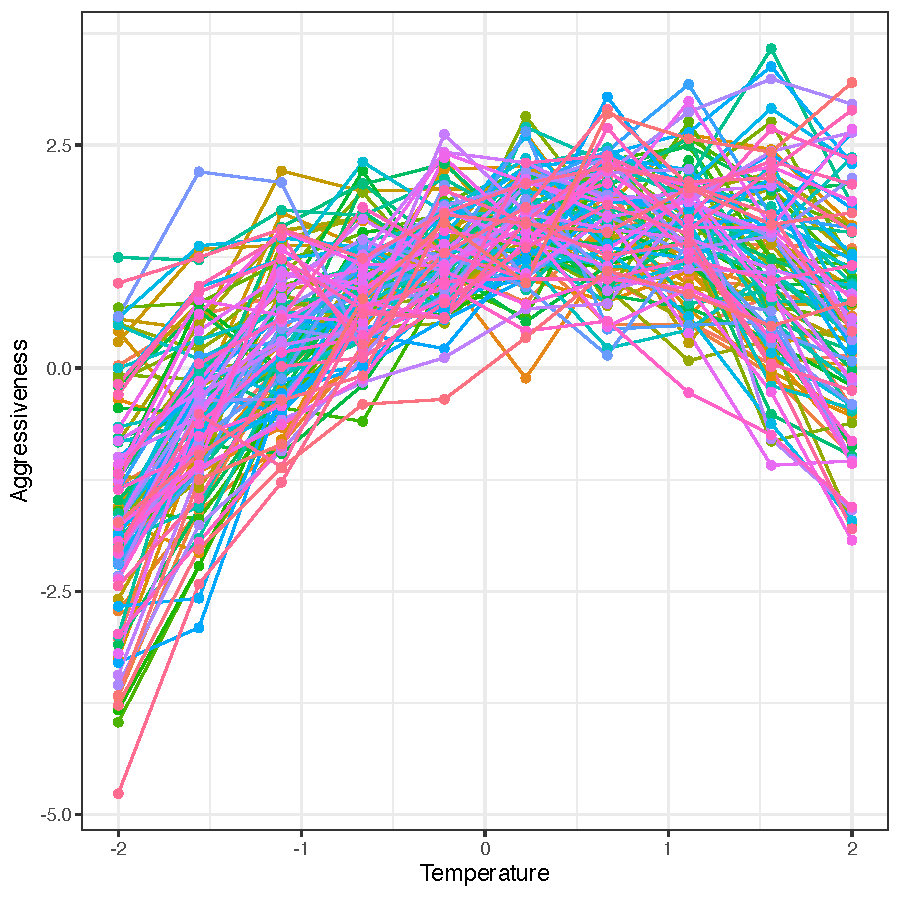
\includegraphics[width = 0.5\textwidth]{Aggressiveness_discrete.pdf}
  \caption{Dragons aggressiveness according to the experimental test temperature}
  \label{fig_agr_rn_plain}
\end{figure}

We can have a look at how aggressiveness depends on the experimental temperature:
\begin{Rinput}
ggplot(dragon_discrete) +
    geom_line(aes(x = Env, y = Aggressiveness, group = Individual, colour = Individual)) +
    geom_point(aes(x = Env, y = Aggressiveness, group = Individual, colour = Individual)) +
    theme(legend.position = "none") +
    xlab("Temperature") + ylab("Aggressiveness")
\end{Rinput}
\autoref{fig_agr_rn_plain} shows the resulting graph, in which we can see that a quadratic curve will probably be a good fit for the reaction norm curve. So, this is what we'll use.

In order to compute a quadratic reaction norm, we have to compute the (mean-centered) squared values of the environment. To be sure to remember that we modified the original \texttt{dragon\_discrete}, we will create a new dataset (say \texttt{tbl\_dragon\_ds})
\begin{Rinput}
tbl_dragon_ds <-
    dragon_discrete |>
    mutate(Env_Sq = (Env - mean(Env))^2)
\end{Rinput}
The mean-centering is necessary to have squared values that are not correlated with the direct environmental values\footnote{Although it is a bit useless here, because the mean is already 0, but better be safe than sorry.}.

\subsubsection{Fitting a quadratic reaction norm to the data}
\label{subsubsec_agr_ds_model}

\paragraph{Running the model}
We will be using the brms package to study (see \autoref{subsec_brms} for more information) to study this quadratic reaction norm.
As a reminder, we will run the model for 3000 iterations in total, discarding the first 1000 iterations considered as lost during the warming-up. Since the NUTS algorithm is particularly efficient to reduce auto-correlation, we will conserve all consecutive iterations:
\begin{Rinput}
# Number of independent chains
n_chains <- 4
# Total number of iterations
n_iter <- 3000
# Number of iterations that will be discarded for the warm-up
n_warm <- 1000
# Thinning interval
n_thin <- 1
\end{Rinput}
To study a quadratic reaction norm, we will use a linear model\footnote{Yes, the model itself is linear, even though the reaction norm is quadratic, because ``linear'' here must be understood as ``linear in its parameters'', which is the case of polynomial functions.}, with two predictors: the temperature and the squared-value of the temperature.
We also need to specify to the model that each values of the three parameters (intercept, slope, second-order component) vary between individuals.
This will be done with \texttt{brms} syntax to specify random effects, which is close to e.g.\ the \texttt{lme4} package:
\begin{Rinput}
form_quad <- brmsformula(Aggressiveness ~ Temp + Temp_Sq + 
                                        (1 + Temp + Temp_Sq | Individual))
\end{Rinput}
The function \texttt{brmsformula()} generates a formula to pass on the function actually running the model, which is named \texttt{brm()}:
\begin{Rinput}
model_agr <-
  brm(formula   = form_quad,
      data      = tbl_dragon_ds,
      save_pars = save_pars(group = FALSE),
      chains    = n_chains,
      cores     = n_chains,
      seed      = seed,
      iter      = n_iter,
      warmup    = n_warm,
      thin      = n_thin)
\end{Rinput}
To explain what is happening here: we ask \texttt{brm()} to run a model using the formula \texttt{form\_rn}, collecting data from the \texttt{tbl\_dragon\_ds} data.frame. We provide the characteristics of the chains we want \texttt{brms} to run.
Note that we provide the \texttt{seed} to the function, so that the output is reproducible.
Finally, the \texttt{save\_pars = save\_pars(group = FALSE)} tells \texttt{brms} that we do not want the random effects predictors to be saved in the model output, as they take a lot of space and are of no use for us in this tutorial.

\paragraph{Checking the model}
We can have a look at the output of the model using the \texttt{summary()} function:
\begin{Rinput}
summary(model_agr)
\end{Rinput}
\begin{Routput}
 Family: gaussian 
  Links: mu = identity; sigma = identity 
Formula: Aggressiveness ~ Temp + Temp_Sq + (1 + Temp + Temp_Sq | Individual) 
   Data: tbl_dragon_ds (Number of observations: 1000) 
  Draws: 4 chains, each with iter = 3000; warmup = 1000; thin = 1;
         total post-warmup draws = 8000

Multilevel Hyperparameters:
~Individual (Number of levels: 100) 
                       Estimate Est.Error l-95% CI u-95% CI Rhat Bulk_ESS
sd(Intercept)              0.28      0.04     0.21     0.35 1.00     4031
sd(Temp)                   0.42      0.03     0.36     0.49 1.00     2350
sd(Temp_Sq)                0.18      0.02     0.14     0.22 1.00     2390
cor(Intercept,Temp)       -0.21      0.13    -0.46     0.05 1.00      751
cor(Intercept,Temp_Sq)    -0.04      0.16    -0.34     0.28 1.00     1347
cor(Temp,Temp_Sq)          0.08      0.12    -0.16     0.32 1.00     2662
                       Tail_ESS
sd(Intercept)              5617
sd(Temp)                   4027
sd(Temp_Sq)                4029
cor(Intercept,Temp)        1588
cor(Intercept,Temp_Sq)     2467
cor(Temp,Temp_Sq)          4250

Regression Coefficients:
          Estimate Est.Error l-95% CI u-95% CI Rhat Bulk_ESS Tail_ESS
Intercept     1.48      0.04     1.41     1.55 1.00     6669     6685
Temp          0.53      0.04     0.44     0.61 1.00     2196     3530
Temp_Sq      -0.49      0.02    -0.53    -0.45 1.00     3527     5341

Further Distributional Parameters:
      Estimate Est.Error l-95% CI u-95% CI Rhat Bulk_ESS Tail_ESS
sigma     0.49      0.01     0.46     0.52 1.00     5206     6387

Draws were sampled using sampling(NUTS). For each parameter, Bulk_ESS
and Tail_ESS are effective sample size measures, and Rhat is the potential
scale reduction factor on split chains (at convergence, Rhat = 1).
\end{Routput}
Beyond the classical values of point estimate, standard error and 95\% CI provided for each parameter of the value, we get values to assess whether the algorithm went well \autocite{vehtari_ranknormalization_2021}.
Notably, $\hat{R}$ tests for convergence (i.e.\ whether the chains reached stationary state) and should near 1 (recommended values are $\hat{R} \leq 1.01$)
The Bulk and Tail effective sample sizes (ESS) provide information regarding whether the chains were long enough to obtain precise estimates or not.
Schematically, the ESS of a chain is the equivalent number of pure Monte Carlo sampling yielding the same amount of information.
In other words, if you had 1000 iterations, but an ESS of 40, it is \textit{as if} you drew only 40 independent samples from the posterior distribution of the parameter.
The reason for this discrepancy comes from the fact that consecutive iterations in the chains are not independent (there is auto-correlation).
While Bulk ESS provides information on how well we sampled around the mean (so, how well it is estimated), Tail ESS provides information on how well we sampled the tail (so, how well the variance is estimated).
Both ESS should be above at least 400 for all parameters \autocite{vehtari_ranknormalization_2021}.

We can also have a graphical look at the model, to see the traces (values of the parameters along the iterations, to check for convergence) and posterior distributions of the parameters (see \autoref{fig_mod_agr}):
\begin{Rinput}
plot(model_agr)
\end{Rinput}

\begin{figure}[t!h!]
  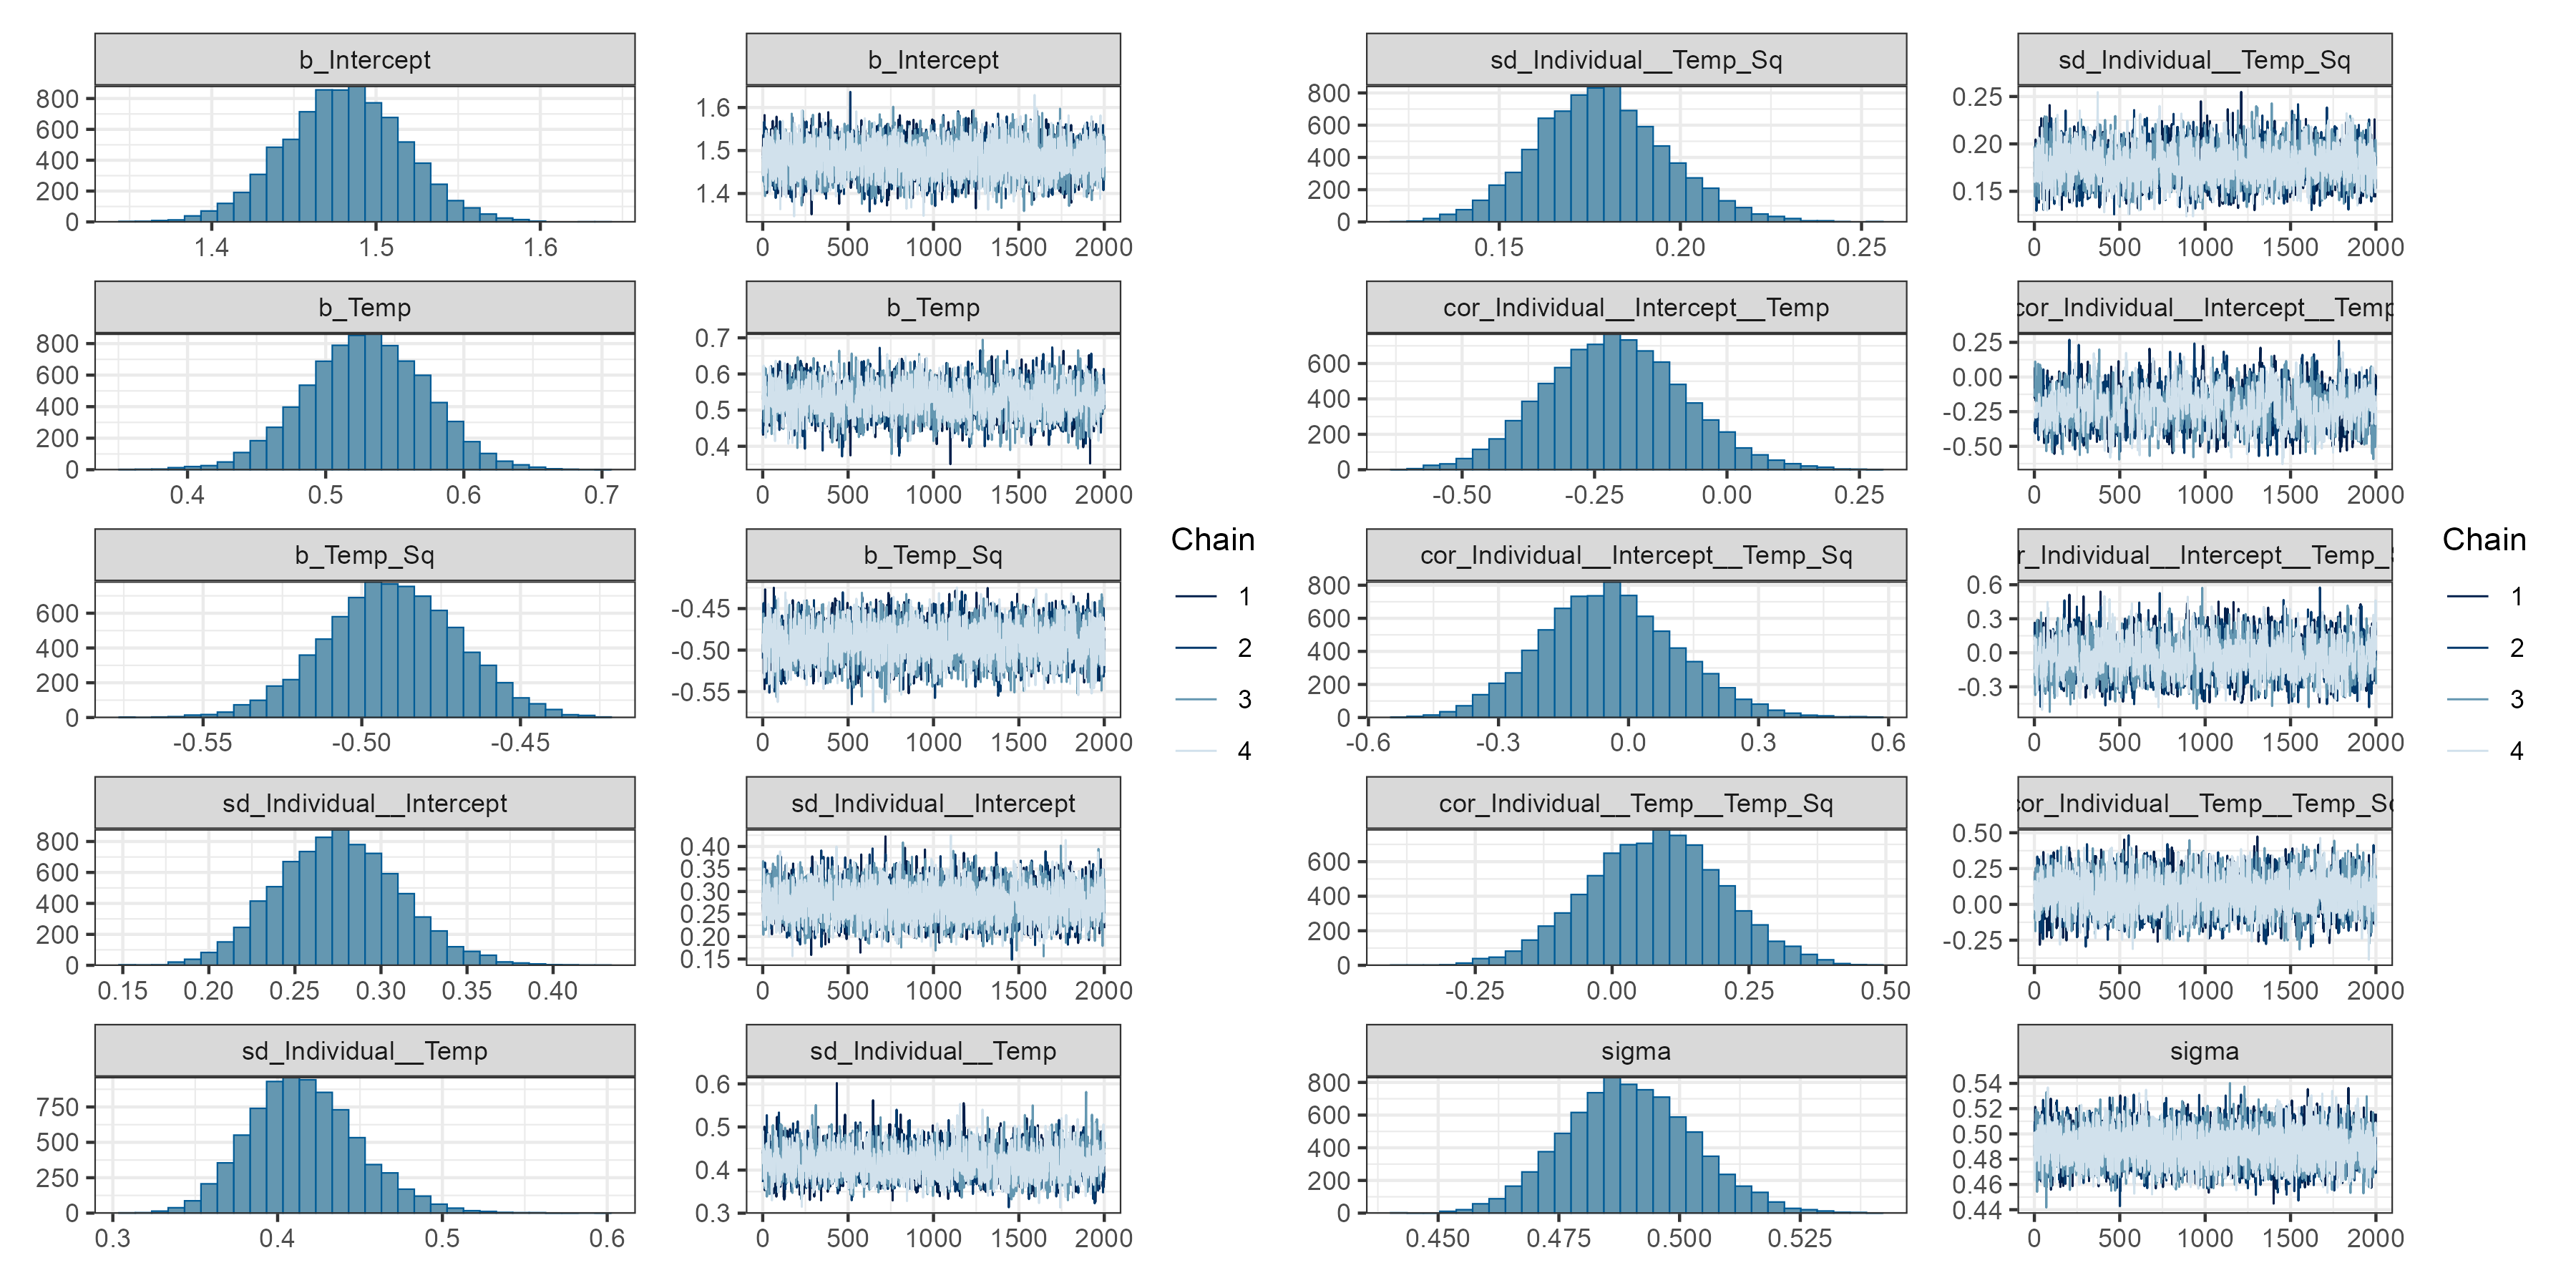
\includegraphics[width = \textwidth]{Aggressiveness_discrete_model.png}
  \caption{Plot of the \texttt{mod\_agr} model. Parameters starting with ``b'' are the fixed effects parameters of the model, and parameters starting with ``sd'' are the standard deviation of the random effects. The parameter ``sigma'' is the residual standard deviation.}
  \label{fig_mod_agr}
\end{figure}

To have a better look at how the model fits the data, we can have a look at the average reaction norm predicted by the model:
\begin{Rinput}
tbl_agr_mod <-
    tbl_dragon_ds |>
    mutate(Predict = predict(model_agr, re_formula = NA) |>
                     as_tibble()) |>
    unpack(Predict) |>
    select(Temp,
           Predict = Estimate,
           Predict_Low = Q2.5,
           Predict_Up  = Q97.5) |>
    summarise(across(starts_with("Predict"), mean),
              .by = Temp)

p_rn_agr <-
    p_aggr +
    geom_ribbon(data = tbl_agr_mod,
                mapping = aes(x = Temp, ymin = Predict_Low, ymax = Predict_Up),
                alpha = 0.3) +
    geom_line(data = tbl_agr_mod,
              mapping = aes(x = Temp, y = Predict),
              linewidth = 1)
\end{Rinput}

\begin{figure}[h!]
  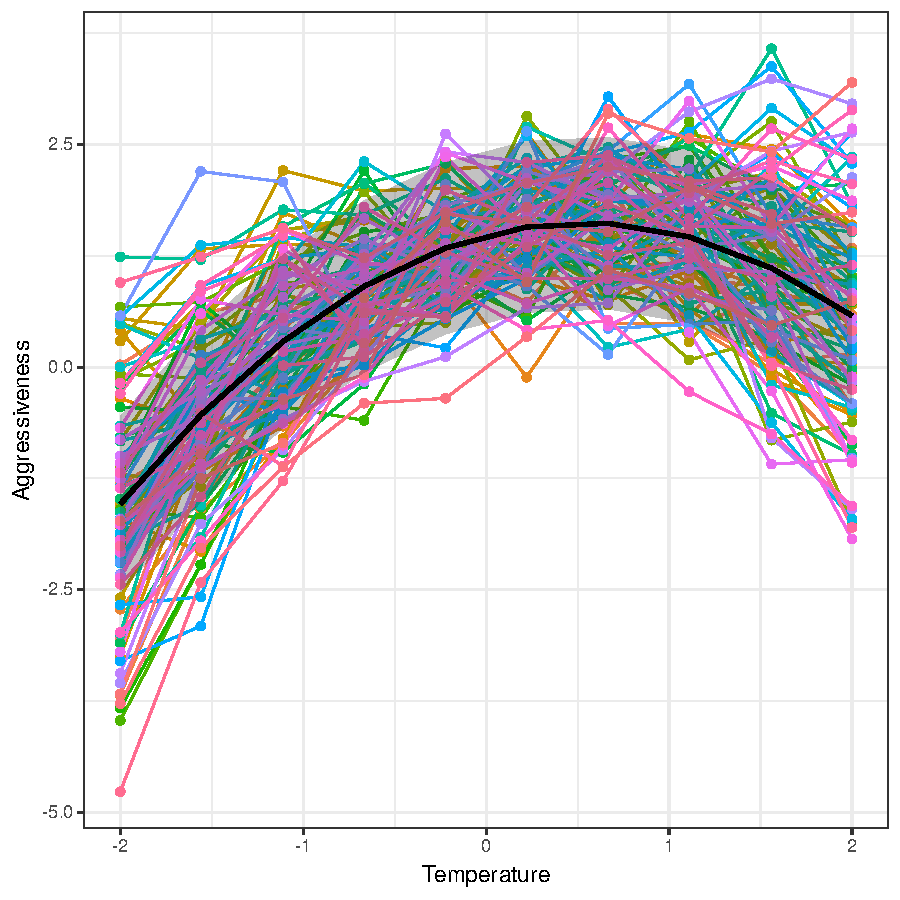
\includegraphics[width = 0.7\textwidth]{Aggressiveness_discrete_pred.pdf}
  \caption{Aggressiveness individual data, with the average reaction norm predicted by the \texttt{mod\_agr} model.}
  \label{fig_pred_agr}
\end{figure}

\subsubsection{Decomposing the variance based on point estimates}

\paragraph{Getting point estimates}
In order to perform the variance decomposition using the \texttt{Reacnorm} package, we need first to extract the point estimates of key parameters in the model. The first thing we will need are the estimates of the quadratic coefficients of the model ($\bar{\theta}$ in the theoretical overview above). To do so, we will use the \texttt{fixef()} function:
\begin{Rinput}
theta_agr <- fixef(model_agr, robust = TRUE)[ , "Estimate"]
names(theta_agr) <- c("a", "b", "c")
theta_agr
\end{Rinput}
\begin{Routput}
         a          b          c 
 1.4808551  0.5293001 -0.4903728 
\end{Routput}
Similarly, we can extract the variance-covariance of the fitted random effects:
\begin{Rinput}
G_agr <-
    VarCorr(model_agr, robust = TRUE)[["Individual"]][["cov"]][ , "Estimate", ]
rownames(G_agr) <- colnames(G_agr) <- names(theta_agr)
G_agr
\end{Rinput}
\begin{Routput}
             a            b            c
a  0.075549554 -0.023922259 -0.002332428
b -0.023922259  0.171736042  0.005871739
c -0.002332428  0.005871739  0.031550777
\end{Routput}
Note that we used the \texttt{robust = TRUE} argument. This outputs the posterior median, rather than the more classical posterior mean, as a point estimate. In general, if the posterior distribution is symmetrical (see ``b'' prefixed panels in \autoref{fig_mod_agr}), both point estimates should be comparable.
But for standard-deviations or variances of the random effects, posterior distributions tend to be strongly to slightly asymmetrical, in which case the posterior median is a better point estimate.
We thus use \texttt{robust = TRUE} everywhere for consistency.
We can also extract the residual variance, that will be useful to get at the total phenotypic variance contained in the reaction norm:
\begin{Rinput}
vr_agr <- VarCorr(model_agr, robust = TRUE)[["residual__"]][["sd"]][ , "Estimate"]^2
vr_agr
\end{Rinput}
\begin{Routput}
[1] 0.2394762
\end{Routput}
Finally, we will require the uncertainty around the $\bar{\theta}$ point estimates, i.e.\ the $\mathbf{S}$ matrix (see theoretical overview):
\begin{Rinput}
S_theta_agr <- vcov(model_agr)
rownames(S_theta_agr) <- colnames(S_theta_agr) <- c("a", "b", "c")
S_theta_agr
\end{Rinput}
\begin{Routput}
              a             b             c
a  0.0013203047 -0.0003068121 -0.0002255506
b -0.0003068121  0.0019102726  0.0000669430
c -0.0002255506  0.0000669430  0.0004393123
\end{Routput}

\paragraph{Design matrix}
The last ingredient we will require to use the \texttt{Reacnorm} package is the design matrix $\mathbf{X}$ is the linear model. Unfortunately, \texttt{brms} objects do not contain such matrix, but we can ``reconstruct'' it based on the formula of the model, using the \texttt{model.matrix()} function:
\begin{Rinput}
design_mat <- model.matrix(Aggressiveness ~ Temp + Temp_Sq, data = tbl_dragon_ds)
head(design_mat)
\end{Rinput}
\begin{Routput}
  (Intercept) Temp Temp_Sq
1           1   -2       4
2           1   -2       4
3           1   -2       4
4           1   -2       4
5           1   -2       4
6           1   -2       4
\end{Routput}

\paragraph{Getting the variance of average reaction norm and its decomposition}
In order to obtain the variance of the average reaction norm ($V_{\text{Plas}}$) and its decomposition, the simplest and quickest way is to use the \texttt{rn\_phi\_decomp()} function :
\begin{Rinput}
plas_agr <-
    rn_phi_decomp(theta = theta_agr, X = design_mat, S = S_theta_agr)
plas_agr
\end{Rinput}
\begin{Routput}
     V_Plas     Phi_b     Phi_c      Phi_b_c
1 0.9497063 0.4781417 0.5218583 7.671419e-17
\end{Routput}
Since the true reaction norm is quadratic, we know that the $\varphi$- and $\pi$-decomposition are equal, and thus, here we have $\varphi_{b}=\pi_{\text{Sl}}$ and $\varphi_{c}=\pi_{\text{Cv}}$.
Hence, the function performing the $\pi$-decomposition would yield (approximately) the same result.
However, because it requires performing numerical integration, it would take longer (roughly 200 times longer, but still instant here) and be slightly less exact:
\begin{Rinput}
plas_agr_pi <-
    rn_pi_decomp(th eta   = theta_agr,
                 G_theta = G_agr,
                 env     = tbl_dragon_ds[["Temp"]] |> unique(),
                 shape   = expression(a + b * x + c * x^2))
plas_agr_pi
\end{Rinput}
\begin{Routput}
     V_Plas    Pi_Sl     Pi_Cv
1 0.9537137 0.478577 0.5205334
\end{Routput}
There are two reasons for why the two functions slightly differ. The first is that, while \texttt{rn\_phi\_decomp()} accounts for the uncertainty in $\bar{\theta}$ using the $\mathbf{S}$ matrix, the \texttt{rn\_pi\_decomp()} function cannot do it. If we were to not provide $\mathbf{S}$ when calling \texttt{rn\_phi\_decomp()}, the results would be even close to \texttt{rn\_pi\_decomp()}:
\begin{Rinput}
rn_phi_decomp(theta = theta_agr, X = design_mat)
\end{Rinput}
\begin{Routput}
     V_Plas     Phi_b     Phi_c      Phi_b_c
1 0.9537309 0.4793928 0.5206072 7.639302e-17
\end{Routput}
The second reason is that \texttt{rn\_phi\_decomp()} uses exact matrix computation, while \texttt{rn\_pi\_decomp()} is based on numerical integration, which is (slightly) more approximative.
In the end, we can claim that $V_{\text{Plas}}=0.95$, with $\pi_{\text{Sl}}=0.48$ and $\pi_{\text{Cv}}=0.52$.
The variance $V_{\text{Plas}}$ is the variance arising from variation along the black line in \autoref{fig_pred_agr}. 
Slightly more of this variance is coming from the curvature of this line ($\pi_{\text{Cv}}=0.52$) than from its average slope ($\pi_{\text{Sl}}=0.48$), although these contributions are close to equality.

\paragraph{Getting the additive genetic variances and their decomposition}
To compute the additive genetic variance of the reaction norm ($V_{\text{Add}}$) and its $\gamma$-decomposition; the marginal additive genetic variance of the trait ($V_{\text{A}}$); and the additive genetic variance of plasticity ($V_{\text{A}\times\text{E}}$) and its $\iota$-decomposition.
\begin{Rinput}
gen_agr <-
    rn_gen_decomp(theta = theta_agr, G_theta = G_agr, X = design_mat)
gen_agr
\end{Rinput}
\begin{Routput}
      V_Add       V_A     V_AxE   Gamma_a   Gamma_b   Gamma_c Gamma_a_b Gamma_b_c
1 0.4973828 0.1519671 0.3454157 0.1518942 0.5634872 0.2999246         0         0
    Gamma_a_c Iota_a    Iota_b    Iota_c Iota_a_b Iota_a_c Iota_b_c
1 -0.01530597      0 0.8113958 0.1886042        0        0        0
\end{Routput}
The additive genetic variance of the reaction is thus $V_{\text{Add}} = 0.50$), so roughly twice as low as $V_{\text{Plas}}$.
It is composed for a third by the marginal additive genetic variance of the trait ($V_{\text{A}} = 0.15$) and for two-thirds by the additive genetic variance of plasticity ($V_{\text{A}\times\text{E}} = 0.35$).
This seems to suggest that there is a considerable amount of adaptive potential in the plasticity of aggressiveness.
Most of the additive genetic variation in the reaction norm comes from variation in the slopes ($\gamma_{b}=0.56$). Regarding genetic variation in plasticity itself, it is even more the case that most of the variation (thus adaptive potential) comes from the slope ($\iota_{b}=0.81$).
Note that, in this simple case, most of the covariance terms (e.g.\ $\gamma_{a,b}=0$ or $\iota_{b,c}=0$).
For the sake of security, the \texttt{Reacnorm} function will always yield all components even if they are null.
In the rest of this tutorial, we will remove such null elements by imposing a threshold. For this, we will use the \texttt{select()} function from \texttt{dplyr}:
\begin{Rinput}
rn_gen_decomp(theta = theta_agr, G_theta = G_agr, X = design_mat) |>
    select(where( \§§(col_) { abs(mean(col_)) > 10^-5 }) ) 
\end{Rinput}
\begin{Routput}
      V_Add       V_A     V_AxE   Gamma_a   Gamma_b   Gamma_c   Gamma_a_c
1 0.4973828 0.1519671 0.3454157 0.1518942 0.5634872 0.2999246 -0.01530597
     Iota_b    Iota_c
1 0.8113958 0.1886042
\end{Routput}
Less cluttered, uh?

\paragraph{Computing the total phenotypic variance and the variance-standardised estimates}
Now that we have everything, we can finally compute the total phenotypic variance in the reaction norm:
\begin{Rinput}
v_tot_agr <- plas_agr[["V_Plas"]] + gen_agr[["V_Add"]] + vr_agr
v_tot_agr
\end{Rinput}
\begin{Routput}
[1] 1.686565
\end{Routput}
By dividing $V_{\text{Plas}}$, $V_{\text{Add}}$, $V_{\text{A}}$ and $V_{\text{A}\times\text{E}}$, we can obtain the variance-standardised estimates $P^{2}_{\text{RN}}$, $h^{2}_{\text{RN}}$, $h^{2}$ and $h^{2}_{\text{I}}$:
\begin{Rinput}
v_tot_agr <- plas_agr[["V_Plas"]] + gen_agr[["V_Add"]] + vr_agr
var_agr <-
    c(P2     = plas_agr[["V_Plas"]] / v_tot_agr,
      h2_RN  = gen_agr[["V_Add"]] / v_tot_agr,
      h2     = gen_agr[["V_A"]] / v_tot_agr,
      h2_I   = gen_agr[["V_AxE"]] / v_tot_agr,
      T2     = (plas_agr[["V_Plas"]] + gen_agr[["V_Add"]]) / v_tot_agr)
var_agr
\end{Rinput}
\begin{Routput}
        P2      h2_RN         h2       h2_I         T2 
0.56310083 0.29490873 0.09010449 0.20480423 0.85800955 
\end{Routput}
As we mentioned above, the contribution of the variance arising from plasticity due to the average reaction norm is larger than the contribution of the total additive genetic variance (i.e.\ $P^{2}_{\text{RN}} = 0.56 > 0.29 = h^{2}_{\text{RN}}$).
This also illustrate one of the fundamental results of the companion paper \autocite{devillemereuil_general_2016}, i.e.\ $h^{2}_{\text{RN}} = h^{2} + h^{2}_{\text{I}}$.
The reaction norm explains a large part of the total phenotypic variance ($T^{2}_{\text{RN}}=0.86$).

\subsubsection{Decomposing the variance using the full posterior distribution}
\label{subsubsec_agr_ds_post}

\paragraph{Getting the posterior distributions of the parameters}
Getting estimates from the point estimates of the model is a nice first thing, but it is not the best (Bayesian) way to obtain our variance decomposition. It is better to compute the above parameter from each iteration of our model's chains.
In order to do so, we will first have to collect the values of our parameters for each iterations of the chain.
We will do so by setting the argument \texttt{summary = FALSE} in the functions that we used above:
\begin{Rinput}
theta_post_agr <- fixef(model_agr, summary = FALSE)
colnames(theta_post_agr) <- c("a", "b", "c")
head(theta_post_agr)
\end{Rinput}
\begin{Routput}
    variable
draw        a         b          c
   1 1.488025 0.4744503 -0.5005814
   2 1.511379 0.4318258 -0.5009057
   3 1.521973 0.4587290 -0.4994489
   4 1.532942 0.4816476 -0.5069072
   5 1.537320 0.4673945 -0.4882447
   6 1.501262 0.4572999 -0.5282360
\end{Routput}
\begin{Rinput}
G_post_agr <-
    VarCorr(model_agr, summary = FALSE)[["Individual"]][["cov"]] |>
    # We use apply() to transform the 3-dimensional array into a list
    apply(1, \§§(mat_) { mat_ }, simplify = FALSE) |>
    map( \§§(mat_) { rownames(mat_) <- colnames(mat_) <- c("a", "b", "c"); return(mat_) })
G_post_agr[[1]]
\end{Rinput}
\begin{Routput}
            a            b           c
a  0.07372066 -0.018482854 0.008082450
b -0.01848285  0.192524723 0.005297588
c  0.00808245  0.005297588 0.028833529
\end{Routput}
\begin{Rinput}
vr_post_agr <-
    VarCorr(model_agr, summary = FALSE)[["residual__"]][["sd"]][ , 1]^2
head(vr_post_agr)
\end{Rinput}
\begin{Routput}
        1         2         3         4         5         6 
0.2574979 0.2319611 0.2425255 0.2417751 0.2719007 0.2292515 
\end{Routput}
To transform those into posterior chains, we will use the package \texttt{posterior}:
\begin{Rinput}
post_agr <- as_draws_df(theta_post_agr)
post_agr[["G"]] <- G_post_agr
post_agr[["V_R"]] <- vr_post_agr
post_agr
\end{Rinput}
\begin{Routput}
# A draws_df: 2000 iterations, 4 chains, and 5 variables
     a    b     c
1  1.5 0.47 -0.50
2  1.5 0.43 -0.50
3  1.5 0.46 -0.50
4  1.5 0.48 -0.51
5  1.5 0.47 -0.49
6  1.5 0.46 -0.53
7  1.5 0.55 -0.49
8  1.5 0.58 -0.47
9  1.5 0.55 -0.47
10 1.5 0.55 -0.53
                                                                                  G  V_R
1          0.0737, -0.0185, 0.0081, -0.0185, 0.1925, 0.0053, 0.0081, 0.0053, 0.0288 0.26
2        0.0649, -0.0061, 0.0103, -0.0061, 0.1964, -0.0015, 0.0103, -0.0015, 0.0233 0.23
3            0.0574, 0.0040, 0.0055, 0.0040, 0.2056, 0.0043, 0.0055, 0.0043, 0.0218 0.24
4          0.0811, 0.0080, -0.0034, 0.0080, 0.1684, 0.0061, -0.0034, 0.0061, 0.0306 0.24
5 6.7e-02, -8.2e-05, 4.7e-03, -8.2e-05, 1.6e-01, 1.5e-02, 4.7e-03, 1.5e-02, 2.5e-02 0.27
6 0.0698, -0.00548, -0.00811, -0.00548, 0.186, -0.00077, -0.00811, -0.00077, 0.0296 0.23
7          0.0625, -0.0058, 0.0085, -0.0058, 0.1668, 0.0107, 0.0085, 0.0107, 0.0419 0.24
8          0.0636, -0.0196, 0.0049, -0.0196, 0.2080, 0.0071, 0.0049, 0.0071, 0.0331 0.25
9   0.06724, -0.00861, -0.00063, -0.00861, 0.185, 0.011, -0.00063, 0.01109, 0.03672 0.22
10         0.0907, -0.0192, 0.0024, -0.0192, 0.2508, 0.0134, 0.0024, 0.0134, 0.0387 0.25
# ... with 7990 more draws
# ... hidden reserved variables {'.chain', '.iteration', '.draw'}
\end{Routput}
We can agree that this is not the best output format for the $\mathbf{G}$-matrix...

\paragraph{Subsetting the parameters}
As we can see from the output above, we have 8000 iterations. We could them all, but for the sake of computation time for this tutorial, we will subset to only 1000 iterations of the chains. To do so, we will again use the \texttt{posterior} package to ``thin'' the chains so that we end up with 1000 iterations :
\begin{Rinput}
post_agr <- thin_draws(post_agr, thin = nrow(theta_post_agr) / 1000)
\end{Rinput}
In order to be able to re-transform the future data.frames that we will generate, we will keep the ``meta-information'' that the \texttt{posterior} package keeps at supplementary columns starting with a dot (\texttt{.chain}, \texttt{.iteration}, \texttt{.draw}):
\begin{Rinput}
post_agr_info <- select(post_agr, starts_with("."))
\end{Rinput}

\paragraph{Getting the variance of average reaction norm and its decomposition}
To use the full posterior distribution of the parameters, we need to apply the \texttt{rn\_phi\_decomp()} to each iteration of the chains. To do so, we will use \texttt{apply()}:
\begin{Rinput}
post_plas_agr <-
    post_agr |>
    select(a, b, c) |>
    apply(1, \§§(th_) rn_phi_decomp(theta = th_, X = design_mat, S = S_theta_agr)) |>
    # Collect the output of apply() into a data.frame
    bind_rows()  |>
    select(where( \§§(col_) { abs(mean(col_)) > 10^-5 })) |>
    # Transform this into a "draws" object using posterior package
    cbind(post_agr_info) |>
    as_draws_df()
summarise_draws(post_plas_agr)
\end{Rinput}
\begin{Routput}
# A tibble: 3 × 10
  variable  mean median     sd    mad    q5   q95  rhat ess_bulk ess_tail
  <chr>    <dbl>  <dbl>  <dbl>  <dbl> <dbl> <dbl> <dbl>    <dbl>    <dbl>
1 V_Plas   0.957  0.957 0.0834 0.0850 0.831 1.09  1.00     1012.     908.
2 Phi_b    0.480  0.478 0.0485 0.0481 0.405 0.557 0.999    1050.     933.
3 Phi_c    0.520  0.522 0.0485 0.0481 0.443 0.595 0.999    1050.     933.
\end{Routput}
The nice thing with the way we re-created a ``draws'' object from \texttt{posterior} is that we can compute diagnostic values of our parameters (see columns \texttt{rhat}, \texttt{ess\_bulk} and \texttt{ess\_tail}).
The values for $V_{\text{Plas}}$ is slightly larger than when we used the point estimates, because by averaging over the posterior distribution, due to the averaging over the posterior distribution\footnote{Briefly, the issue is that $V_{\text{Plas}}$ is a variance over the fixed effects estimates, so by averaging over the posterior distribution, part of the uncertainty in these fixed effects estimates is ``absorbed'' into $V_{\text{Plas}}$. This time, it is not possible to simply use the $\mathbf{S}$ variance-covariance matrix correction, because the influence of the prior distribution is such that we are not sure to be over-correcting or not.}.
This time, we also obtain information about uncertainty in the estimates, as well as their 95\% credible interval.
We can also plot graphics of the trace of these derived parameters, as well as their full posterior distribution (see \autoref{fig_agr_var_decomp_ds}) using the \texttt{bayesplot} package :
\begin{Rinput}
mcmc_trace(post_gen_agr)
mcmc_areas(post_gen_agr,
           regex_pars = "^V",
           prob = 0.95,
           area_method = "scaled height") /
    mcmc_areas(post_gen_agr,
               regex_pars = "^[^V]",           # = Not starting with V
               prob = 0.95,
               area_method = "scaled height")
\end{Rinput}
Note that we separated\footnote{Yes, that is the role of \texttt{/} between the two calls to \texttt{mcmc\_areas()}, a syntax provided by the awesome \texttt{patchwork} package to combine plots!} the plot into the actual variance on the one hand, and the $\pi$-decomposition\footnote{Yes, here we used \texttt{rn\_phi\_decomp()} and \texttt{Phi} is printed on the plot, but remember that since the reaction norm is fully quadratic, we have $\pi_{\text{Sl}} = \varphi_b$ and $\pi_{\text{Cv}} = \varphi_c$.} on the other hand.


\begin{figure}
  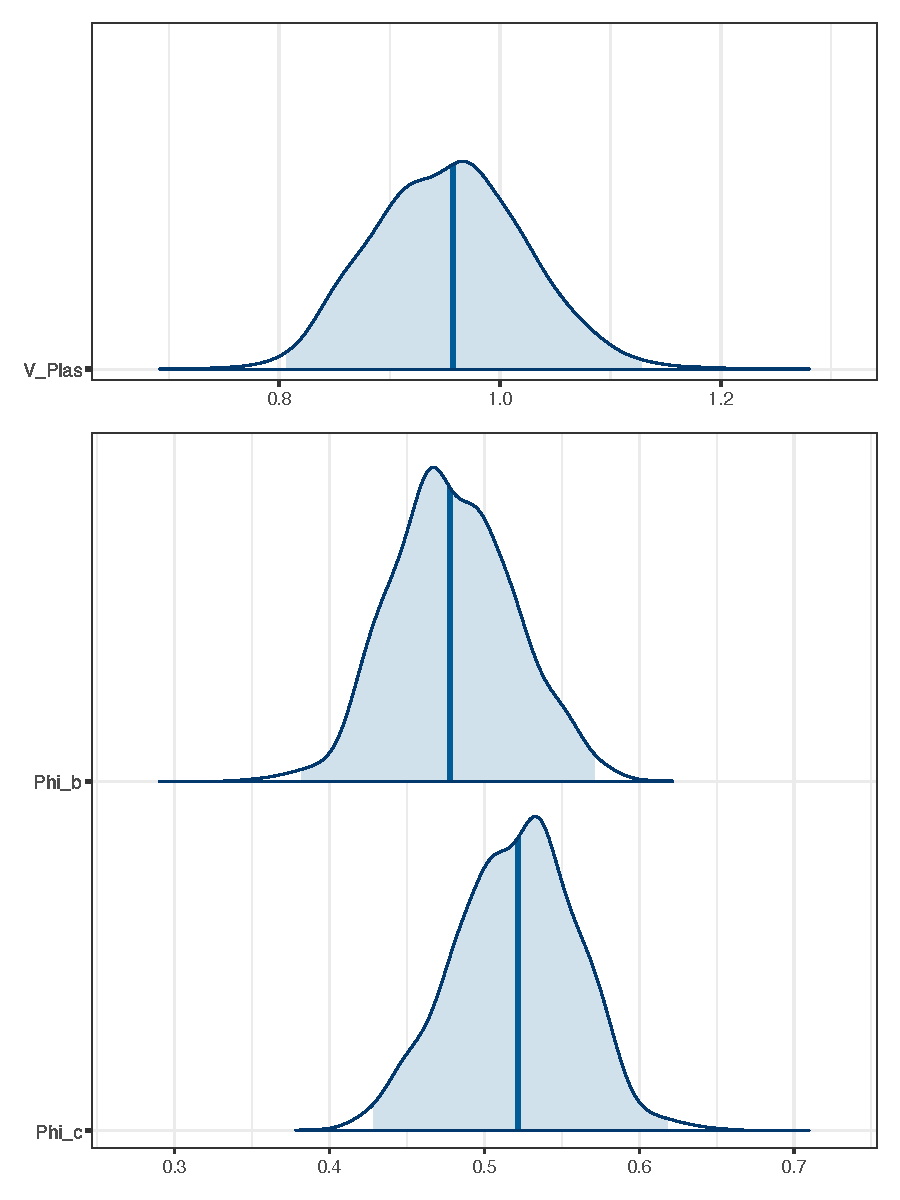
\includegraphics[width = 0.49\textwidth]{Aggressiveness_plas_ds.pdf}
  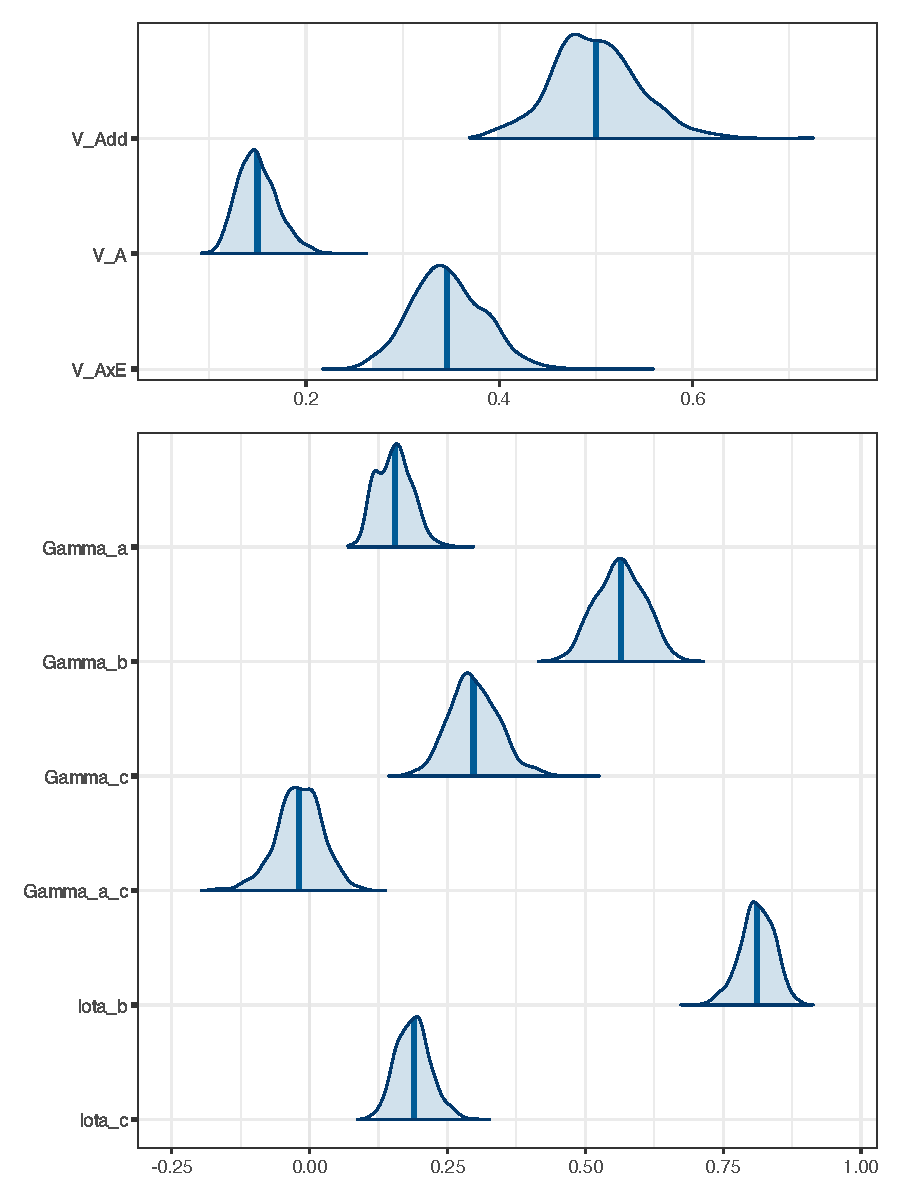
\includegraphics[width = 0.49\textwidth]{Aggressiveness_gen_ds.pdf}
  \caption{Posterior distribution of the variance decomposition of the reaction norm of aggressiveness, based on a quadratic model.}
  \label{fig_agr_var_decomp_ds}
\end{figure}


\paragraph{Getting the additive genetic variances and their decomposition}
Again, to compute the additive genetic variances and their decomposition, we again need to execute the same function over all iterations. But this time, since we will need to iterate over the arguments \texttt{theta} ($\bar{\theta}$) and \texttt{G\_theta} ($\mathbf{G}_{\theta}$) of \texttt{rn\_gen\_decomp()}, we need to be able to use several columns at once.
To do so, we will first prepare a new column for $\bar{\theta}$ in our posterior draws:
\begin{Rinput}
post_agr[["theta"]] <-
    post_agr |>
    select(a:c) |>
    apply(1, \§§(vec_) { vec_ }, simplify = FALSE)
\end{Rinput}
Now, we can use the function \texttt{map2()} from the \texttt{purrr} package from the tidyverse, to apply \texttt{rn\_gen\_decomp()} to both columns at once:
\begin{Rinput}
post_gen_agr <-
    map2(post_agr[["theta"]], post_agr[["G"]],
     \§§(th_, G_) { rn_gen_decomp(theta = th_,
                                G_theta = G_,
                                X = design_mat |> unique()) },
     .progress = TRUE) |>   # This makes map2() prints a nice progress bar
    bind_rows() |>
    select(where(\§§(col_) { abs(mean(col_)) > 10^-5 })) |>
    cbind(post_agr_info) |>
    as_draws_df()
summarise_draws(post_gen_agr)
\end{Rinput}
\begin{Routput}
# A tibble: 9 × 10
  variable     mean  median     sd    mad     q5    q95  rhat ess_bulk ess_tail
  <chr>       <dbl>   <dbl>  <dbl>  <dbl>  <dbl>  <dbl> <dbl>    <dbl>    <dbl>
1 V_Add      0.502   0.500  0.0556 0.0528  0.411 0.599  0.999     933.    1067.
2 V_A        0.153   0.150  0.0257 0.0248  0.116 0.200  1.00      765.     677.
3 V_AxE      0.349   0.346  0.0466 0.0463  0.275 0.427  0.998     897.    1033.
4 Gamma_a    0.156   0.155  0.0383 0.0417  0.100 0.222  0.999    1037.    1035.
5 Gamma_b    0.564   0.564  0.0519 0.0551  0.482 0.647  1.00      815.     933.
6 Gamma_c    0.301   0.297  0.0557 0.0547  0.216 0.403  1.00      834.     947.
7 Gamma_a_c -0.0211 -0.0189 0.0524 0.0482 -0.115 0.0613 1.00      790.    1012.
8 Iota_b     0.810   0.811  0.0387 0.0388  0.739 0.869  1.00      826.     878.
9 Iota_c     0.190   0.189  0.0387 0.0388  0.131 0.261  1.00      826.     878.
\end{Routput}
Here, again, we can also plot the traces and posterior distributions of these derived parameters (see \autoref{fig_agr_var_decomp_ds} for the latter):
\begin{Rinput}
mcmc_trace(post_gen_agr)
mcmc_areas(post_gen_agr,
           regex_pars = "^V",
           prob = 0.95,
           area_method = "scaled height") /
    mcmc_areas(post_gen_agr,
               regex_pars = "^[^V]",
               prob = 0.95,
               area_method = "scaled height")
\end{Rinput}
The point estimates are very close to what we obtained with their direct computation from the point estimates from the model, but here, we have the full posterior of these variance decomposition, and can e.g.\ compute their 95\% credible interval.

\paragraph{Getting the variance-standardised estimates}
If we want to compute the variance-standardised estimates of our variance-decomposition (i.e.\ $P^{2}_{\text{RN}}$, $h^{2}_{\text{RN}}$, $h^{2}$ and $h^{2}_{\text{I}}$), we will need to compute the total phenotypic variance in the reaction norm. An elegant way to do so is to construct a \texttt{posterior} draws object containing all the variance parameters:
\begin{Rinput}
post_var_agr <-
    bind_draws(post_agr, post_plas_agr, post_gen_agr) |>
    subset_draws(variable = c("V_Plas", "V_Add", "V_A", "V_AxE", "V_R")) |>
    mutate_variables(V_Tot = V_Plas + V_Add + V_R)
post_var_agr
\end{Rinput}
\begin{Routput}
# A draws_df: 250 iterations, 4 chains, and 6 variables
   V_Plas V_Add  V_A V_AxE  V_R V_Tot
1    0.88  0.55 0.18  0.37 0.26   1.7
2    0.93  0.54 0.16  0.38 0.22   1.7
3    0.99  0.44 0.13  0.31 0.25   1.7
4    0.97  0.46 0.15  0.32 0.25   1.7
5    1.12  0.54 0.16  0.38 0.25   1.9
6    0.87  0.53 0.13  0.41 0.24   1.6
7    1.06  0.48 0.17  0.31 0.25   1.8
8    0.90  0.58 0.20  0.37 0.22   1.7
9    0.89  0.60 0.21  0.39 0.27   1.8
10   0.91  0.57 0.23  0.34 0.25   1.7
# ... with 990 more draws
# ... hidden reserved variables {'.chain', '.iteration', '.draw'}
\end{Routput}
Then, we can produce a table of all the parameters divided by the total phenotypic variance of the reaction norm (we will use \texttt{transmute()} from \texttt{dplyr} in this case, to automatically get rid of the old columns, but this means we have to make our dataset a \texttt{posterior} object again):
\begin{Rinput}
post_std_agr <-
    post_var_agr |>
    transmute(P2    = V_Plas / V_Tot,
              H2_RN = V_Add / V_Tot,
              H2    = V_A / V_Tot,
              H2_I  = V_AxE / V_Tot,
              T2    = (V_Plas + V_Add) / V_Tot) |>
    cbind(post_agr_info) |>
    as_draws_df()

summarise_draws(post_std_agr)
mcmc_trace(post_std_agr)
mcmc_areas(post_std_agr,
           prob = 0.95,
           area_method = "scaled height")
\end{Rinput}
\begin{Routput}
# A tibble: 5 × 10
  variable   mean median     sd    mad     q5   q95  rhat ess_bulk ess_tail
  <chr>     <dbl>  <dbl>  <dbl>  <dbl>  <dbl> <dbl> <dbl>    <dbl>    <dbl>
1 P2       0.563  0.564  0.0283 0.0289 0.515  0.607 0.997     921.     915.
2 H2_RN    0.295  0.294  0.0272 0.0274 0.252  0.341 0.998     898.     895.
3 H2       0.0900 0.0883 0.0146 0.0148 0.0686 0.116 1.00      706.     882.
4 H2_I     0.205  0.204  0.0235 0.0224 0.170  0.246 0.998     898.    1021.
5 T2       0.858  0.859  0.0109 0.0113 0.840  0.876 0.999    1023.     953.
\end{Routput}

\begin{figure}[h!t!b!]
  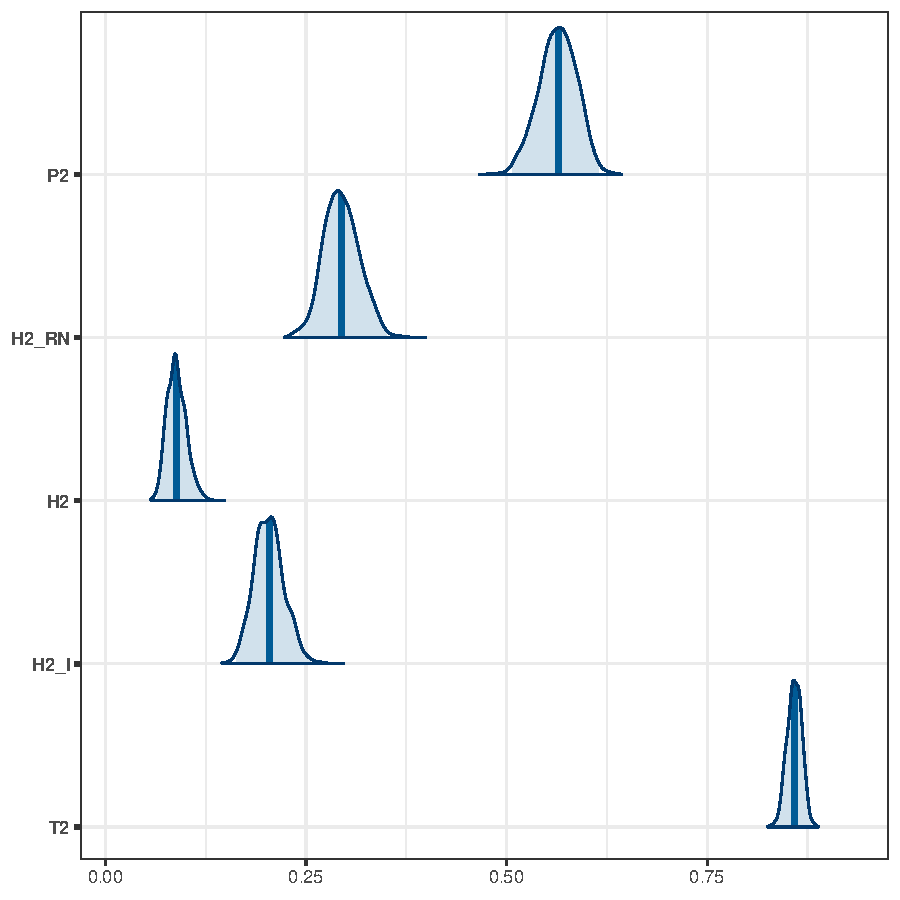
\includegraphics[width = 0.49\textwidth]{Aggressiveness_varstd_ds.pdf}
  \caption{Posterior distribution of the variance-standardised estimates of our variance decomposition of the reaction norm of aggressiveness, based on a quadratic model.}
  \label{fig_agr_var_decomp_ds}
\end{figure}

\subsection{Analysing a non-linear reaction norm with a quadratic curve}

\subsubsection{Overview of the data on performance}

The data on performance can be found, yet again, in the \texttt{dragon\_discrete} dataset shipped with the \texttt{Reacnorm package}, that we transformed into \texttt{tbl\_dragon\_ds} (see the \texttt{Performance} column):
\begin{Rinput}
  head(tbl_dragon_ds)
\end{Rinput}
\begin{Routput}
  Name_Env Temp Individual Aggressiveness Performance Temp_Sq
1   Env_01   -2     Ind_01        -2.1600     -0.0234       4
2   Env_01   -2     Ind_02        -3.0300      0.0564       4
3   Env_01   -2     Ind_03         0.0278      0.0565       4
4   Env_01   -2     Ind_04        -1.3200      0.0744       4
5   Env_01   -2     Ind_05        -3.6800      0.0515       4
6   Env_01   -2     Ind_06        -2.7200     -0.0668       4
\end{Routput}
They are data providing a measure of locomotive performance of the dragons measured at different temperatures. Locomotive performance is measured as the maximum sprint speed attained by individuals, when stimulated with a dummy princess at the end of a very long (thermostatic) corridor.

\begin{figure}[b!h!t!]
  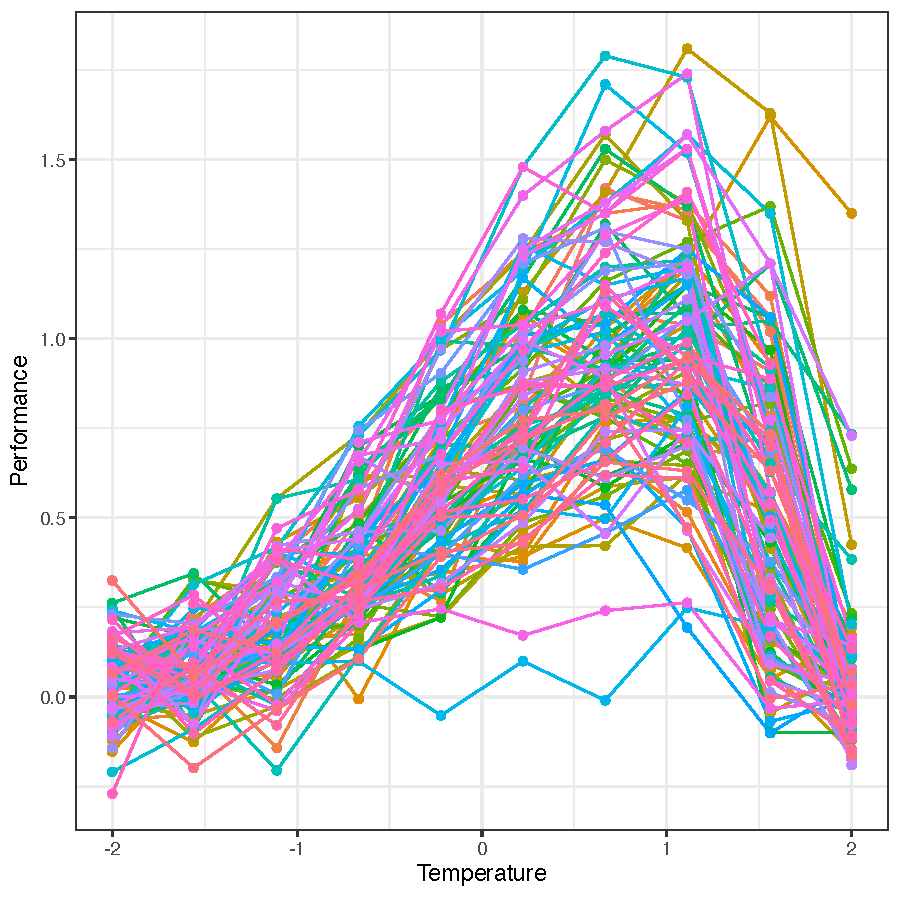
\includegraphics[width = 0.5\textwidth]{TPC_discrete.pdf}
  \caption{Dragons thermal performance, measured as locomotive performance,  according to the experimental test temperature}
  \label{fig_tpc_rn_plain}
\end{figure}

As for aggressiveness, we can have a look at how thermal performance depends on the experimental temperature:
\begin{Rinput}
p_tpc <-
    ggplot(tbl_dragon_ds) +
    geom_line(aes(x = Temp, y = Performance, group = Individual, colour = Individual)) +
    geom_point(aes(x = Temp, y = Performance, group = Individual, colour = Individual)) +
    theme(legend.position = "none") +
    xlab("Temperature") + ylab("Performance")
\end{Rinput}
\autoref{fig_tpc_rn_plain} shows the resulting graph. Clearly, a quadratic curve will not be a perfect fit in this case. We will, however, make do with a quadratic reaction norm to start with, to be able to understand the average variation in terms of slope and curvature. We will measure the level of error we are making by comparing our model with a more general character-state approach, and by computing the $M^{2}_{\text{Plas}}$ introduced in the companion article. 

\subsubsection{Fitting a quadratic reaction norm to the data}

\paragraph{Running the model}
The model is run exactly as in \autoref{subsubsec_agr_ds_model}, although here we will use the column \texttt{Performance} as the response variable:
\begin{Rinput}
form_quad <- brmsformula(Performance ~ Temp + Temp_Sq +
                                       (1 + Temp + Temp_Sq | Individual))
model_tpc_quad <-
    brm(formula   = form_quad,
        data      = tbl_dragon_ds,
        save_pars = save_pars(group = FALSE),
        chains    = n_chains,
        cores     = n_chains,
        seed      = seed,
        iter      = n_iter,
        warmup    = n_warm,
        thin      = n_thin)
\end{Rinput}
This model should take approximately the same amount of time to run as \texttt{model\_agr} previously.

\paragraph{Checking the model}
We first need to check that everything went well by looking at the model summary:
\begin{Rinput}
summary(model_tpc_quad)
\end{Rinput}
\begin{Routput}
 Family: gaussian 
  Links: mu = identity; sigma = identity 
Formula: Performance ~ Temp + Temp_Sq + (1 + Temp + Temp_Sq | Individual) 
   Data: tbl_dragon_ds (Number of observations: 1000) 
  Draws: 4 chains, each with iter = 3000; warmup = 1000; thin = 1;
         total post-warmup draws = 8000

Multilevel Hyperparameters:
~Individual (Number of levels: 100) 
                       Estimate Est.Error l-95% CI u-95% CI Rhat Bulk_ESS Tail_ESS
sd(Intercept)              0.20      0.02     0.16     0.24 1.00     3007     4285
sd(Temp)                   0.06      0.01     0.04     0.08 1.00     4355     5811
sd(Temp_Sq)                0.05      0.01     0.04     0.07 1.00     3420     4693
cor(Intercept,Temp)        0.52      0.15     0.22     0.79 1.00     3235     3793
cor(Intercept,Temp_Sq)    -0.88      0.05    -0.96    -0.76 1.00     4780     4768
cor(Temp,Temp_Sq)         -0.10      0.21    -0.51     0.29 1.00     3039     3868

Regression Coefficients:
          Estimate Est.Error l-95% CI u-95% CI Rhat Bulk_ESS Tail_ESS
Intercept     0.74      0.02     0.70     0.79 1.00     2869     4391
Temp          0.12      0.01     0.11     0.14 1.00     5290     5411
Temp_Sq      -0.17      0.01    -0.19    -0.16 1.00     4809     5624

Further Distributional Parameters:
      Estimate Est.Error l-95% CI u-95% CI Rhat Bulk_ESS Tail_ESS
sigma     0.26      0.01     0.25     0.27 1.00     8096     6268

Draws were sampled using sampling(NUTS). For each parameter, Bulk_ESS
and Tail_ESS are effective sample size measures, and Rhat is the potential
scale reduction factor on split chains (at convergence, Rhat = 1).
\end{Routput}
We can also plot the traces and posterior distributions of the parameters of the model (see \autoref{fig_mod_tpc_quad_ds}):
\begin{Rinput}
plot(model_tpc_quad)
\end{Rinput}

\begin{figure}[t!h!]
  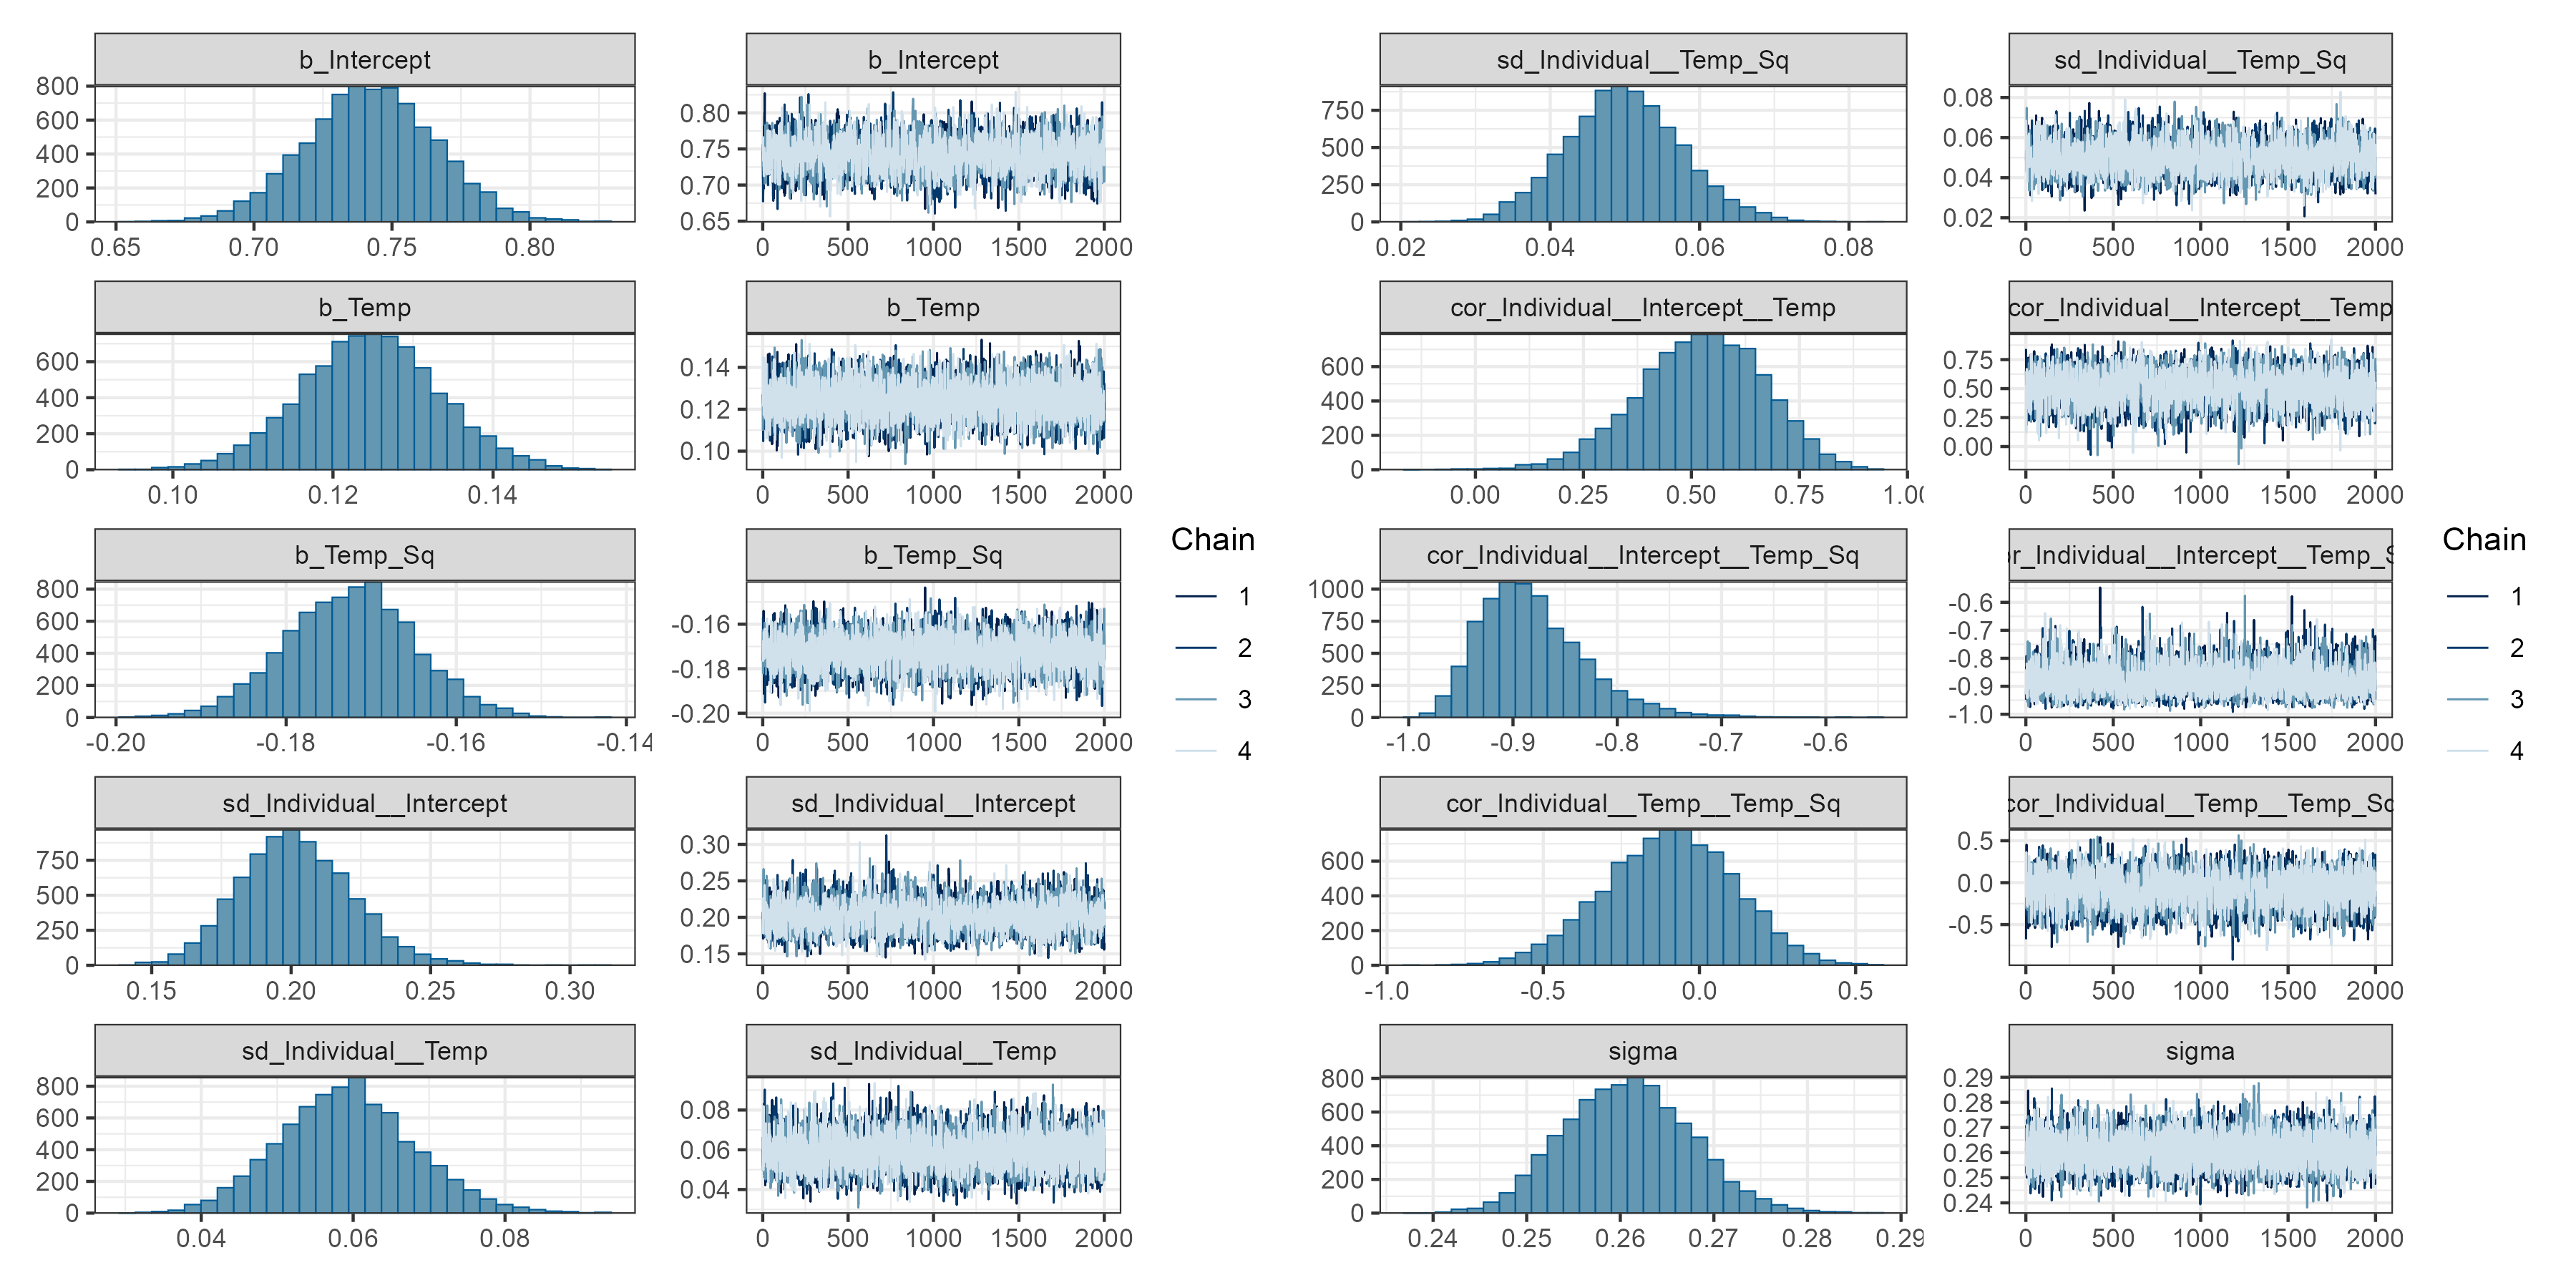
\includegraphics[width = \textwidth]{TPC_discrete_quadratic_model.png}
  \caption{Plot of the \texttt{mod\_tpc\_quad} model. Parameters starting with ``b'' are the fixed effects parameters of the model, and parameters starting with ``sd'' are the standard deviation of the random effects. The parameter ``sigma'' is the residual standard deviation.}
  \label{fig_mod_tpc_quad_ds}
\end{figure}

\begin{figure}[b!h!]
  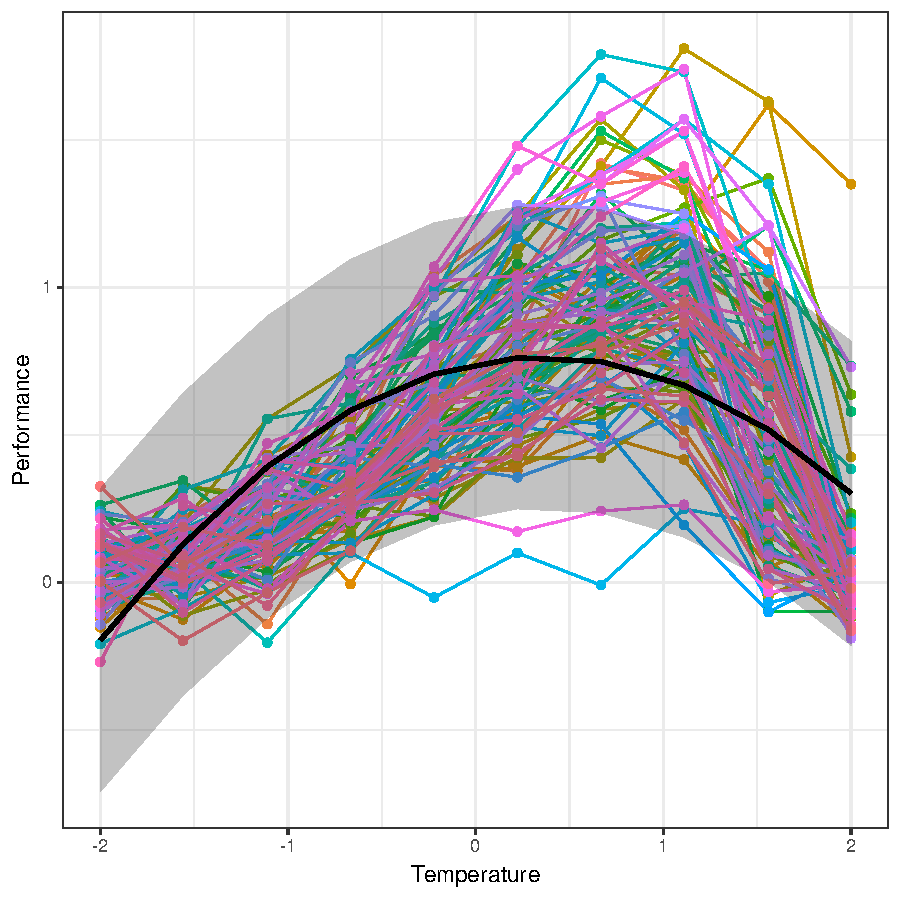
\includegraphics[width = 0.7\textwidth]{TPC_discrete_quadratic_pred.pdf}
  \caption{Fit of the quadratic model of the thermal performance from \texttt{mod\_tpc\_quad}, superimposed over the individual data.}
  \label{fig_pred_agr}
\end{figure}

\paragraph{Looking at the model fit}
We can superimpose the predictions from the quadratic model over the actual reaction norms to visualise how good the fit is to the data (see the results in ):
\begin{Rinput}
tbl_tpc_mod_quad <-
    tbl_dragon_ds |>
    mutate(Predict = predict(model_tpc_quad, re_formula = NA) |>
                     as_tibble()) |>
    unpack(Predict) |>
    select(Temp,
           Predict = Estimate,
           Predict_Low = Q2.5,
           Predict_Up  = Q97.5) |>
    summarise(across(starts_with("Predict"), mean),
              .by = Temp)

p_rn_tpc <-
    p_tpc +
    geom_ribbon(data = tbl_tpc_mod_quad,
                mapping = aes(x = Temp, ymin = Predict_Low, ymax = Predict_Up),
                alpha = 0.3) +
    geom_line(data = tbl_tpc_mod_quad,
              mapping = aes(x = Temp, y = Predict),
              linewidth = 1)
\end{Rinput}
Clearly, the fit is not great (notice also the strongest uncertainty than for aggressiveness), but it does get most of the variation in the reaction norm.
We will see how we can quantify this in a more precise way using $M^{2}_{\text{Plas}}$ in a bit below.

\subsubsection{A first variance decomposition}

\paragraph{Getting the posterior distributions of the parameters}
We can obtain the full posterior distribution of the parameters the same way as we did for the aggressiveness data\footnote{Note that we will skip using point estimates here, as using the full posterior distribution is generally better, notably because we can assess the uncertainty surrounding our variance decomposition estimates}:
\begin{Rinput}
# Getting the design matrix
design_mat <- model.matrix(Performance ~ Temp + Temp_Sq, data = tbl_dragon_ds)

# Getting the error variance-covariance matrix S_theta
S_theta_tpc <- vcov(model_tpc_quad)
rownames(S_theta_tpc) <- colnames(S_theta_tpc) <- c("a", "b", "c")

# Getting the fixed effects from the model (with the whole posterior distribution)
theta_post_tpc <- fixef(model_tpc_quad, summary = FALSE)
colnames(theta_post_tpc) <- c("a", "b", "c")
# Getting the G-matrix from the random effects variances-covariances 
G_post_tpc <-
    VarCorr(model_tpc_quad, summary = FALSE)[["Individual"]][["cov"]] |>
    apply(1, \§§(mat_) { mat_ }, simplify = FALSE) |>
    map(\§§(mat_) { rownames(mat_) <- colnames(mat_) <- c("a", "b", "c"); return(mat_) })

# Creating a posterior sample using the posterior package
post_tpc <- as_draws_df(theta_post_tpc)
post_tpc[["G"]] <- G_post_tpc
post_tpc[["theta"]] <-
    post_tpc |>
    select(a:c) |>
    apply(1, \§§(vec_) { vec_ }, simplify = FALSE)
# Subsetting the iterations to 1000
post_tpc <- thin_draws(post_tpc, thin = nrow(theta_post_tpc) / 1000)
# Keep the iteration/chain info to create new posterior objects
post_tpc_info <- select(post_tpc, starts_with("."))
\end{Rinput}
We did everything here at once, but the steps are more detailed for the aggressiveness trait in \autoref{subsubsec_agr_ds_post}.

\paragraph{Decomposing the average reaction norm variance}
We used a quadratic function, but we know that it is unlikely that the reaction norm curve truly is quadratic, so, we cannot use the $\pi$-decomposition in this case. We will thus use the $\varphi$-decomposition for good this time:
\begin{Rinput}
post_plas_tpc_quad <-
    post_tpc |>
    select(a, b, c) |>
    apply(1, \§§(th_) rn_phi_decomp(theta = th_, X = design_mat, S = S_theta_tpc)) |>
    bind_rows()  |>
    select(where(\§§(col_) { abs(mean(col_)) > 10^-5 })) |>
    cbind(post_tpc_info) |>
    as_draws_df()

summarise_draws(post_plas_tpc_quad)
\end{Rinput}
\begin{Routput}
# A tibble: 3 × 10
  variable   mean median      sd     mad     q5    q95  rhat ess_bulk ess_tail
  <chr>     <dbl>  <dbl>   <dbl>   <dbl>  <dbl>  <dbl> <dbl>    <dbl>    <dbl>
1 V_Plas   0.0867 0.0865 0.00655 0.00631 0.0761 0.0980  1.00     946.     981.
2 Phi_b    0.290  0.290  0.0340  0.0330  0.234  0.352   1.00     957.     772.
3 Phi_c    0.710  0.710  0.0340  0.0330  0.648  0.766   1.00     957.     772.
\end{Routput}
We cannot directly interpret the $\varphi_{b}$ and $\varphi_{c}$ estimates in terms of the contribution of slope ($\pi_{\text{Sl}}$) and curvature ($\pi_{\text{Cv}}$) in the ``geometric'' sense of the term, because the environment is not normally distributed.
But there's another problem: given that the quadratic curve does not entirely follow the reaction norms, we do not know whether we can trust the estimation of $V_{\text{Plas}}$, so we might want to fit a more applicable model to the data before we analyse anything.

\subsubsection{Fitting a character-state model to the data}
\label{subsubsec_tpc_cs}

\paragraph{Running and checking the model}
The character-state model takes advantage of our discretised environments to analyse the environment as a categorical factor, rather than a continuous one. This way, there is no need to parametrised a curve in advance for the model, as each environmental value will have its own parameter.
To do so, we will change the formula to define the model, using the environment name column (\texttt{Name\_Env}), and pass it to \texttt{brms}:
\begin{Rinput}
form_cs <- brmsformula(Performance ~ 0 + Name_Env + (0 + Name_Env | Individual))
model_cs_tpc <-
    brm(formula   = form_cs,
        data      = tbl_dragon_ds,
        save_pars = save_pars(group = FALSE),
        chains    = n_chains,
        cores     = n_chains,
        seed      = seed,
        iter      = 6000,
        warmup    = 1000,
        thin      = 1)
summary(model_cs_tpc)
\end{Rinput}
\begin{Routput}
 Family: gaussian 
  Links: mu = identity; sigma = identity 
Formula: Performance ~ 0 + Name_Env + (0 + Name_Env | Individual) 
   Data: tbl_dragon_ds (Number of observations: 1000) 
  Draws: 4 chains, each with iter = 6000; warmup = 1000; thin = 1;
         total post-warmup draws = 20000

Multilevel Hyperparameters:
~Individual (Number of levels: 100) 
                                Estimate Est.Error l-95% CI u-95% CI Rhat Bulk_ESS Tail_ESS
sd(Name_EnvEnv_01)                  0.06      0.02     0.02     0.09 1.00     1765     3251
sd(Name_EnvEnv_02)                  0.06      0.01     0.03     0.09 1.00     2718     5557
sd(Name_EnvEnv_03)                  0.11      0.01     0.09     0.14 1.00     5238    11208
sd(Name_EnvEnv_04)                  0.14      0.01     0.11     0.16 1.00     7023    13178
sd(Name_EnvEnv_05)                  0.19      0.01     0.16     0.22 1.00     7363    12646
sd(Name_EnvEnv_06)                  0.24      0.02     0.21     0.28 1.00     6553    11333
sd(Name_EnvEnv_07)                  0.28      0.02     0.24     0.32 1.00     6239     9848
sd(Name_EnvEnv_08)                  0.30      0.02     0.26     0.34 1.00     6859    10767
sd(Name_EnvEnv_09)                  0.39      0.03     0.33     0.44 1.00     8810    11828
sd(Name_EnvEnv_10)                  0.20      0.02     0.17     0.24 1.00     9102    12198
cor(Name_EnvEnv_01,Name_EnvEnv_02)  0.12      0.24    -0.34     0.58 1.00     3369     6169
cor(Name_EnvEnv_01,Name_EnvEnv_03)  0.22      0.19    -0.16     0.58 1.00     2173     3928
cor(Name_EnvEnv_02,Name_EnvEnv_03)  0.30      0.18    -0.07     0.64 1.00     2576     4378
cor(Name_EnvEnv_01,Name_EnvEnv_04)  0.40      0.17     0.05     0.71 1.00     2553     4913
cor(Name_EnvEnv_02,Name_EnvEnv_04)  0.41      0.17     0.07     0.72 1.00     2517     4931
cor(Name_EnvEnv_03,Name_EnvEnv_04)  0.61      0.11     0.37     0.80 1.00     5894     8772
cor(Name_EnvEnv_01,Name_EnvEnv_05)  0.34      0.16     0.01     0.66 1.00     1855     2940
cor(Name_EnvEnv_02,Name_EnvEnv_05)  0.46      0.15     0.15     0.73 1.00     2523     4113
cor(Name_EnvEnv_03,Name_EnvEnv_05)  0.65      0.10     0.44     0.82 1.00     4754     7894
cor(Name_EnvEnv_04,Name_EnvEnv_05)  0.72      0.08     0.55     0.86 1.00     4598     9687
cor(Name_EnvEnv_01,Name_EnvEnv_06)  0.32      0.16     0.02     0.63 1.00     1693     2350
cor(Name_EnvEnv_02,Name_EnvEnv_06)  0.40      0.15     0.09     0.68 1.00     2141     3316
cor(Name_EnvEnv_03,Name_EnvEnv_06)  0.66      0.09     0.48     0.82 1.00     4355     7048
cor(Name_EnvEnv_04,Name_EnvEnv_06)  0.75      0.07     0.60     0.87 1.00     5458    10968
cor(Name_EnvEnv_05,Name_EnvEnv_06)  0.89      0.04     0.80     0.95 1.00     5881    10335
cor(Name_EnvEnv_01,Name_EnvEnv_07)  0.29      0.16    -0.03     0.60 1.00     1668     2143
cor(Name_EnvEnv_02,Name_EnvEnv_07)  0.30      0.15    -0.01     0.59 1.00     2130     3590
cor(Name_EnvEnv_03,Name_EnvEnv_07)  0.48      0.10     0.27     0.67 1.00     4374     7448
cor(Name_EnvEnv_04,Name_EnvEnv_07)  0.64      0.08     0.48     0.78 1.00     6163    11145
cor(Name_EnvEnv_05,Name_EnvEnv_07)  0.79      0.05     0.68     0.88 1.00     5849    10299
cor(Name_EnvEnv_06,Name_EnvEnv_07)  0.86      0.04     0.78     0.93 1.00     5889    11602
cor(Name_EnvEnv_01,Name_EnvEnv_08)  0.15      0.16    -0.16     0.48 1.00     1715     2172
cor(Name_EnvEnv_02,Name_EnvEnv_08)  0.06      0.16    -0.25     0.37 1.00     1956     2961
cor(Name_EnvEnv_03,Name_EnvEnv_08)  0.45      0.10     0.24     0.64 1.00     4189     8169
cor(Name_EnvEnv_04,Name_EnvEnv_08)  0.46      0.09     0.26     0.63 1.00     5904    10000
cor(Name_EnvEnv_05,Name_EnvEnv_08)  0.61      0.07     0.45     0.74 1.00     6915    11837
cor(Name_EnvEnv_06,Name_EnvEnv_08)  0.76      0.05     0.65     0.85 1.00     9471    14779
cor(Name_EnvEnv_07,Name_EnvEnv_08)  0.86      0.04     0.79     0.92 1.00     8228    14263
cor(Name_EnvEnv_01,Name_EnvEnv_09)  0.02      0.17    -0.32     0.35 1.00     1978     3020
cor(Name_EnvEnv_02,Name_EnvEnv_09) -0.22      0.16    -0.52     0.10 1.00     1890     3939
cor(Name_EnvEnv_03,Name_EnvEnv_09) -0.14      0.12    -0.36     0.09 1.00     4826     8989
cor(Name_EnvEnv_04,Name_EnvEnv_09) -0.17      0.11    -0.37     0.05 1.00     5328    11048
cor(Name_EnvEnv_05,Name_EnvEnv_09)  0.02      0.10    -0.17     0.22 1.00     7439    10641
cor(Name_EnvEnv_06,Name_EnvEnv_09)  0.20      0.09     0.02     0.37 1.00     9381    13733
cor(Name_EnvEnv_07,Name_EnvEnv_09)  0.47      0.08     0.31     0.61 1.00    10259    13876
cor(Name_EnvEnv_08,Name_EnvEnv_09)  0.65      0.06     0.52     0.75 1.00    11453    13792
cor(Name_EnvEnv_01,Name_EnvEnv_10) -0.09      0.18    -0.44     0.27 1.00     2048     3081
cor(Name_EnvEnv_02,Name_EnvEnv_10) -0.04      0.17    -0.38     0.29 1.00     1877     2577
cor(Name_EnvEnv_03,Name_EnvEnv_10) -0.18      0.12    -0.42     0.06 1.00     4643     9162
cor(Name_EnvEnv_04,Name_EnvEnv_10) -0.17      0.11    -0.38     0.06 1.00     6007    10506
cor(Name_EnvEnv_05,Name_EnvEnv_10) -0.15      0.10    -0.35     0.06 1.00     8391    13452
cor(Name_EnvEnv_06,Name_EnvEnv_10)  0.01      0.10    -0.19     0.21 1.00     9588    14460
cor(Name_EnvEnv_07,Name_EnvEnv_10)  0.10      0.10    -0.10     0.29 1.00    11711    14658
cor(Name_EnvEnv_08,Name_EnvEnv_10)  0.17      0.10    -0.03     0.36 1.00    13629    16173
cor(Name_EnvEnv_09,Name_EnvEnv_10)  0.54      0.08     0.37     0.68 1.00    13426    16683

Regression Coefficients:
               Estimate Est.Error l-95% CI u-95% CI Rhat Bulk_ESS Tail_ESS
Name_EnvEnv_01     0.04      0.01     0.02     0.06 1.00    18101    15540
Name_EnvEnv_02     0.08      0.01     0.06     0.10 1.00    16308    14263
Name_EnvEnv_03     0.20      0.01     0.17     0.22 1.00     7720    12567
Name_EnvEnv_04     0.37      0.02     0.34     0.40 1.00     6724    11503
Name_EnvEnv_05     0.60      0.02     0.56     0.64 1.00     5497    10036
Name_EnvEnv_06     0.81      0.03     0.76     0.87 1.00     4865     9047
Name_EnvEnv_07     0.95      0.03     0.89     1.01 1.00     4923     8811
Name_EnvEnv_08     0.98      0.03     0.92     1.04 1.00     5091     9087
Name_EnvEnv_09     0.53      0.04     0.45     0.61 1.00     7929    11100
Name_EnvEnv_10     0.05      0.02     0.01     0.10 1.00    10566    12887

Further Distributional Parameters:
      Estimate Est.Error l-95% CI u-95% CI Rhat Bulk_ESS Tail_ESS
sigma     0.09      0.00     0.08     0.10 1.01     1184      582

Draws were sampled using sampling(NUTS). For each parameter, Bulk_ESS
and Tail_ESS are effective sample size measures, and Rhat is the potential
scale reduction factor on split chains (at convergence, Rhat = 1).
\end{Routput}
Note that we had to increase the number of iterations to run the model, because the residual standard deviation had too small efficient sample size and too high $\hat{R}$.
The high number of parameters are due to the fact that, as part of the character-state model, we now infer a $10\times10$ $\mathbf{G}$ matrix, with additive genetic variances and covariances across all pairs of environments.
We can also graphically check that everything went smoothly, but we will only select a few parameters to not overwhelm the graphic (see \autoref{fig_mod_tpc_cs_ds}):
\begin{Rinput}
# We select everything starting with a "b_" (fixed effects) and the residual sd
plot(model_cs_tpc, variable = c("^b_", "sigma"), regex = TRUE)
\end{Rinput}

\begin{figure}[t!h!]
  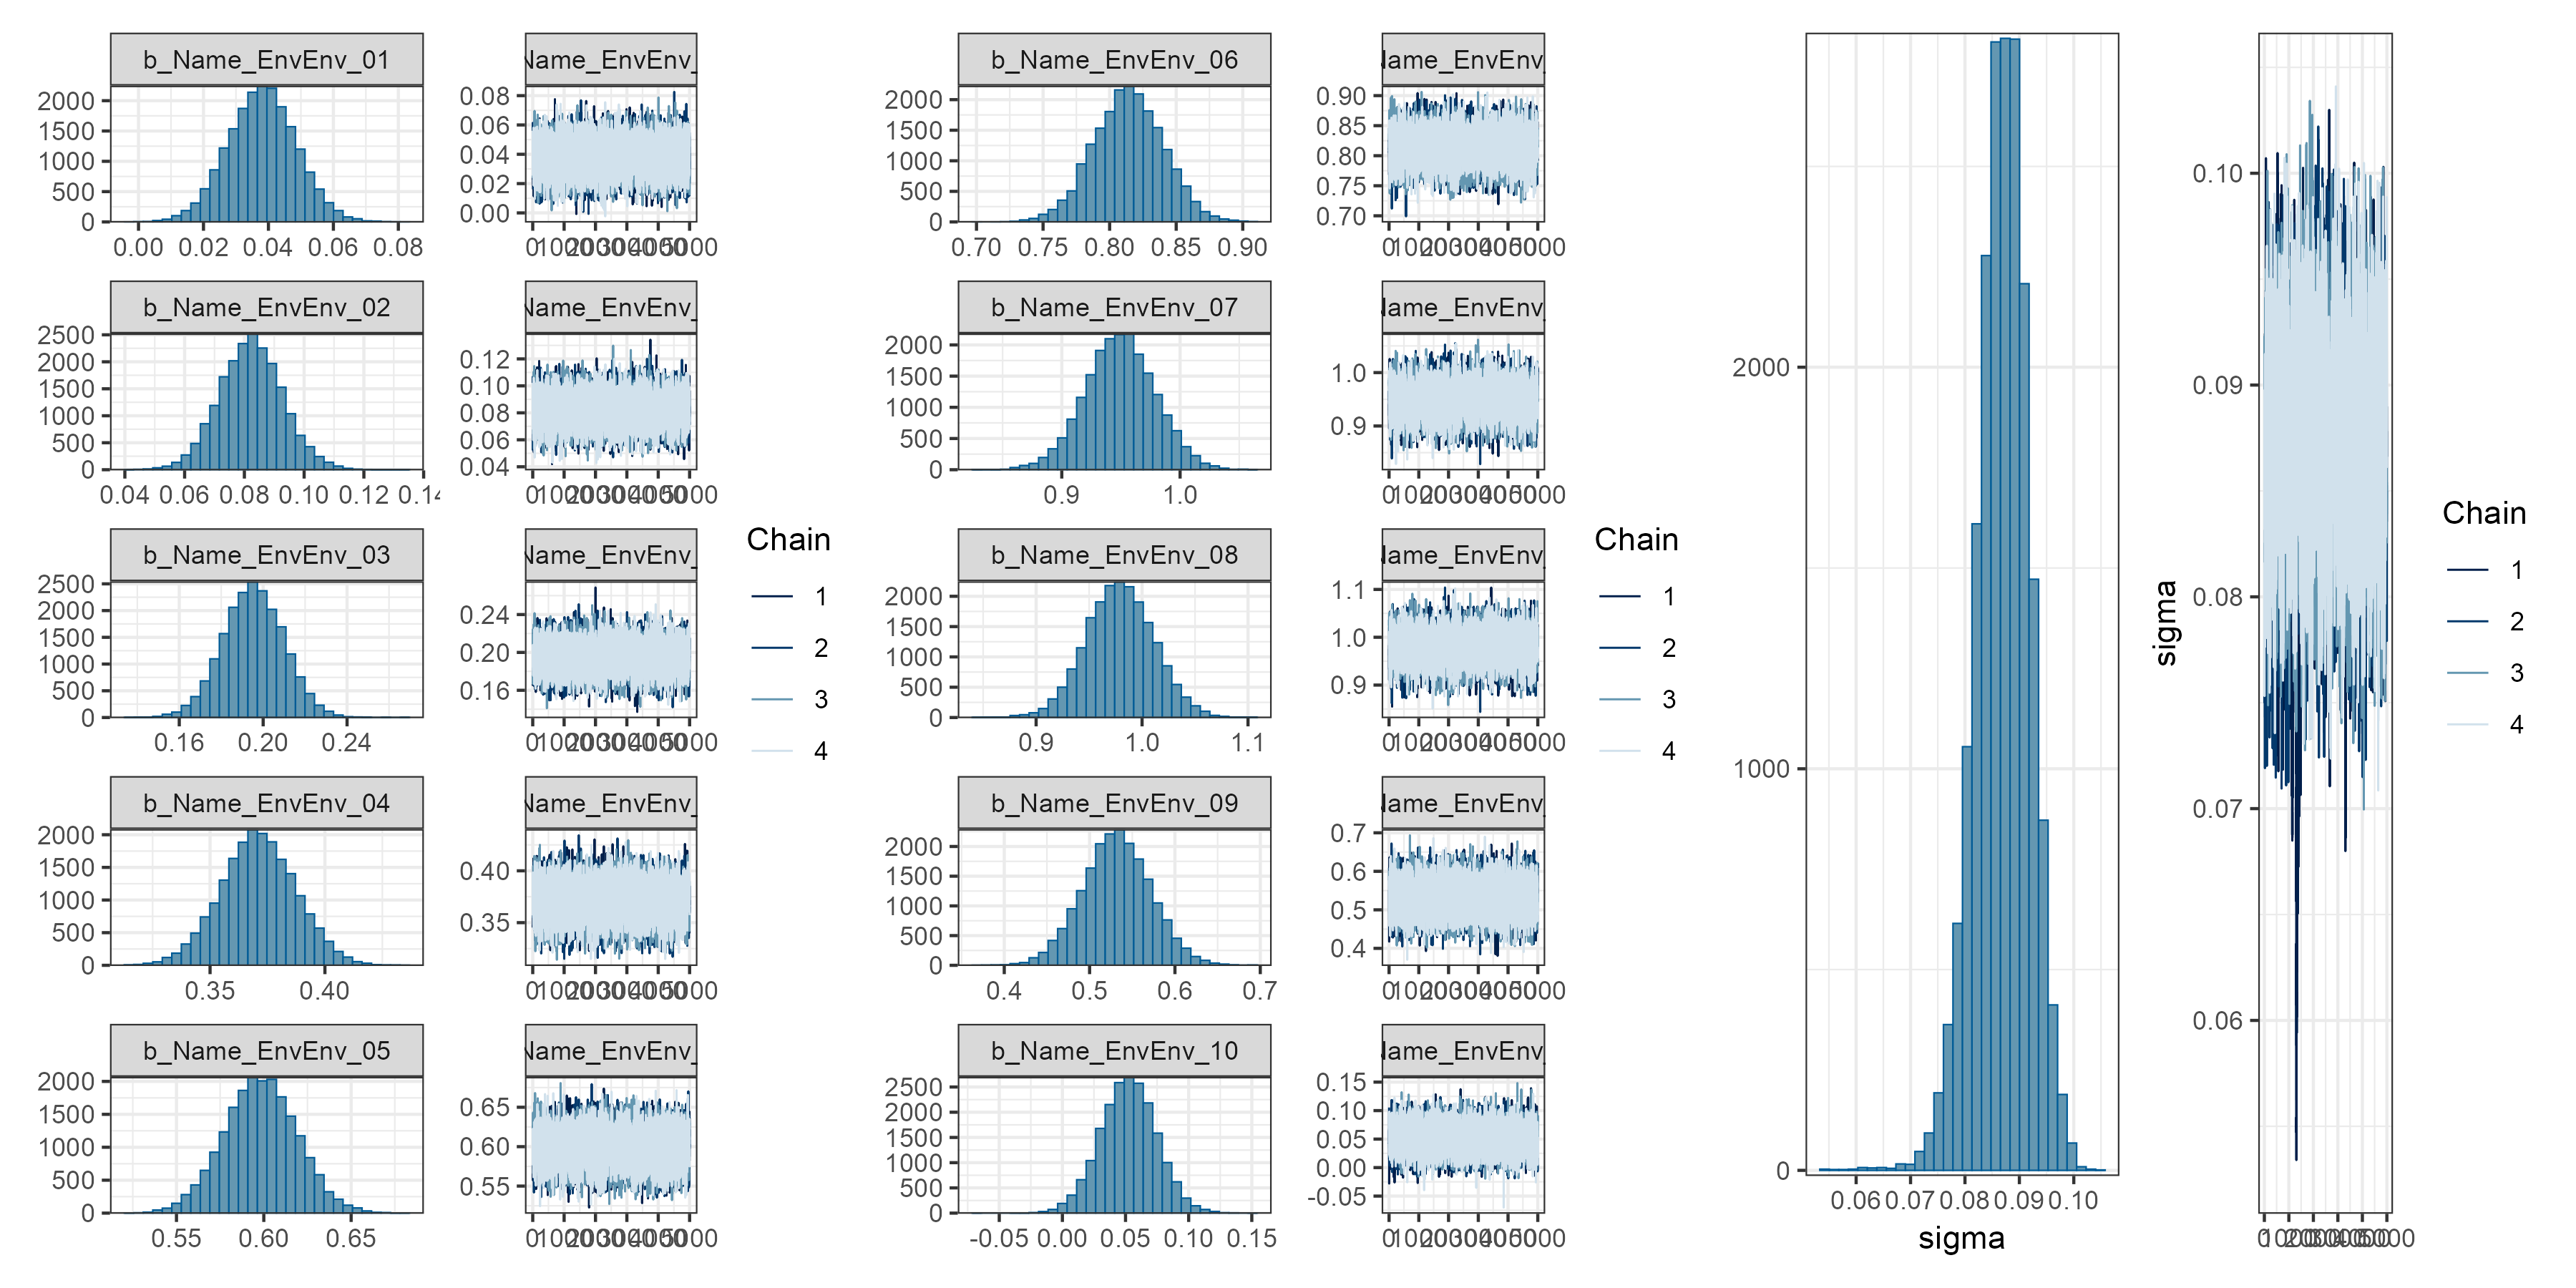
\includegraphics[width = \textwidth]{TPC_discrete_cs_model.png}
  \caption{Plot of the \texttt{mod\_cs\_tpc} model. Parameters starting with ``b'' are the fixed effects parameters of the model. The parameter ``sigma'' is the residual standard deviation.}
  \label{fig_mod_tpc_cs_ds}
\end{figure}

\begin{figure}[b!h!]
  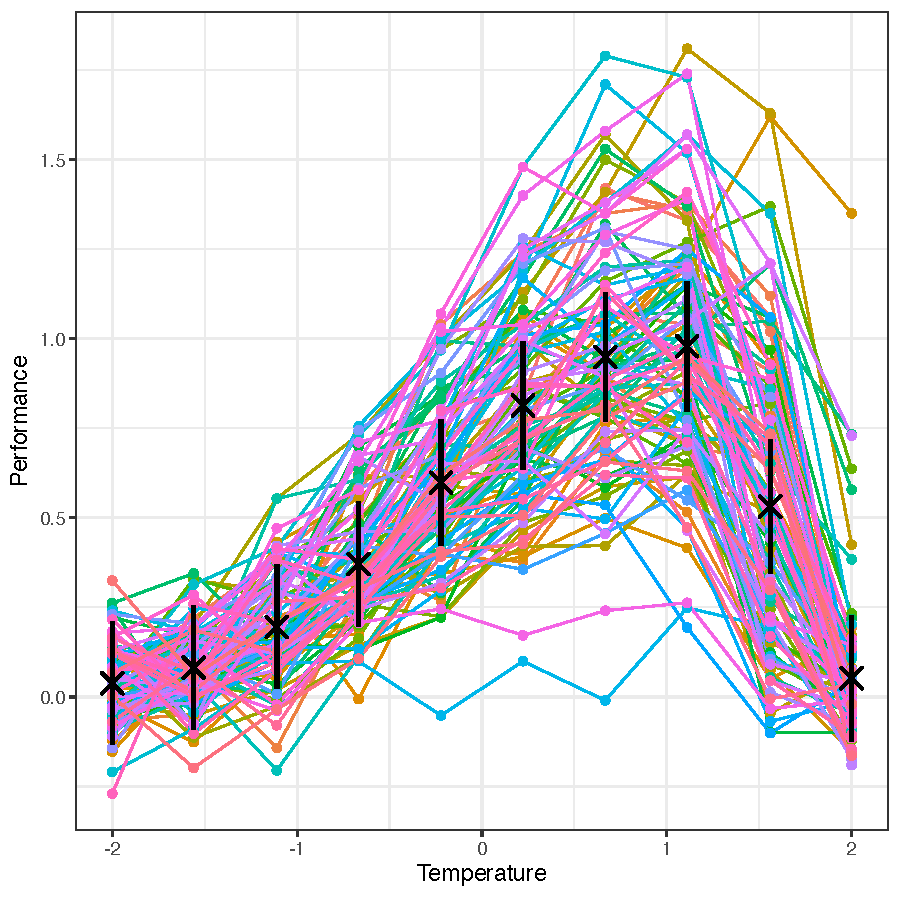
\includegraphics[width = 0.7\textwidth]{TPC_discrete_cs_pred.pdf}
  \caption{Fit of the character-state model of the thermal performance from \texttt{mod\_cs\_tpc}, superimposed over the individual data.}
  \label{fig_pred_cs_tpc}
\end{figure}

Because the character-state does not make explicit assumption about the shape of the curve of the reaction norm, we can see the fit of each point to the global curve is better than the quadratic curve (see \autoref{fig_pred_cs_tpc}):
\begin{Rinput}
tbl_tpc_mod_cs <-
    tbl_dragon_ds |>
    mutate(Predict = predict(model_cs_tpc, re_formula = NA) |>
                     as_tibble()) |>
    unpack(Predict) |>
    select(Temp,
           Predict = Estimate,
           Predict_Low = Q2.5,
           Predict_Up  = Q97.5) |>
    summarise(across(starts_with("Predict"), mean),
              .by = Temp)

p_rn_tpc_cs <-
    p_tpc +
    geom_pointrange(data = tbl_tpc_mod_cs,
                    mapping = aes(x = Temp, y = Predict, ymin = Predict_Low, ymax = Predict_Up),
                    size = 1, linewidth = 1, shape = 4)
\end{Rinput}

\paragraph{Extracting the parameters from the model}
As always, the first thing to do is to extract the parameters of interest from the model.
Since the character-state model is quite straightforward, we can directly extract $V_{\text{Plas}}$ (which is simply the variance of the population-level effects) and the $\mathbf{G}$-matrix.
We will directly extract their posterior distribution this time:
\begin{Rinput}
# Getting the uncertainty on the parameters
var_uncert_cs_tpc <-
    vcov(model_cs_tpc) |>
    diag() |>
    mean()

# Computing V_plas
post_theta_cs <- 
    fixef(model_cs_tpc, summary = FALSE) |>
    as_draws_df()
var_plas_cs <-
    post_theta_cs |>
    select(starts_with("Name")) |>
    as.matrix() |>
    rowVars()

# Correcting for the uncertainty
post_cs <-
    data.frame(V_Plas = var_plas_cs - var_uncert_cs_tpc) |>
    cbind(select(post_theta_cs, starts_with("."))) |>
    as_draws_df()

# Getting the G-matrix
post_cs[["G"]] <-
    VarCorr(model_cs_tpc, summary = FALSE)[["Individual"]][["cov"]] |>
    apply(1, \§§(mat_) { mat_ }, simplify = FALSE)
# Getting the residual variance
post_cs[["V_R"]] <-
    VarCorr(model_cs_tpc, summary = FALSE)[["residual__"]][["sd"]][ , 1]^2
\end{Rinput}
And of course, we will subset the iterations to a thousands, once again:
\begin{Rinput}
post_cs <- thin_draws(post_cs, thin = length(var_plas_cs) / 1000)
post_cs_info <- select(post_cs, starts_with("."))
\end{Rinput}
Let's look at the output for $V_{\text{Plas}}$:
\begin{Rinput}
summarise_draws(subset_draws(post_cs, variable = "V_Plas"))
\end{Rinput}
\begin{Routput}
# A tibble: 1 × 10
  variable  mean median      sd     mad    q5   q95  rhat ess_bulk ess_tail
  <chr>    <dbl>  <dbl>   <dbl>   <dbl> <dbl> <dbl> <dbl>    <dbl>    <dbl>
1 V_Plas   0.136  0.136 0.00841 0.00838 0.122 0.150 0.999     845.    1011.
\end{Routput}
As expected, the variance due to the average reaction norm obtained from the character-state ($V_{\text{Plas}} = 0.136$) is bigger than the one obtained from the quadratic model ($V_{\text{Plas}} = 0.087$), so that we roughly have $M^{2}_{\text{Plas}} =  0.087 / 0.136 = 0.64$.
We will see later how to compute $M^{2}_{\text{Plas}}$ more properly, using the full posterior distribution.

\paragraph{Computing the additive genetic variances from the character-state model}
We can compute the additive genetic variances $V_{\text{Add}}$, $V_{\text{A}}$ and $V_{\text{A}\times\text{E}}$ directly from the $\mathbf{G}$-matrix when using a character-state model.
$V_{\text{Add}}$ is the average of the diagonal elements, while $V_{\text{A}}$ is the average of all elements of the $\mathbf{G}$-matrix.
We can then simply obtain $V_{\text{A}\times\text{E}}$ using the difference between the two variances: $V_{\text{A}\times\text{E}} = V_{\text{Add}} - V_{\text{A}}$.
This is implemented in the \texttt{rn\_cs\_gen()} function of the \texttt{Reacnorm} package:
\begin{Rinput}
post_gen_cs <-
    map(post_cs[["G"]], rn_cs_gen, .progress = TRUE) |>
    bind_rows()  |>
    select(where(\§§(col_) { abs(mean(col_)) > 10^-5 })) |>
    cbind(post_tpc_info) |>
    as_draws_df()

summarise_draws(post_gen_cs)
\end{Rinput}
\begin{Routput}
# A tibble: 4 × 10
  variable   mean median      sd     mad     q5    q95  rhat ess_bulk ess_tail
  <chr>     <dbl>  <dbl>   <dbl>   <dbl>  <dbl>  <dbl> <dbl>    <dbl>    <dbl>
1 V_Add    0.0488 0.0485 0.00461 0.00444 0.0419 0.0567  1.00     959.     949.
2 V_A      0.0182 0.0180 0.00235 0.00225 0.0146 0.0222  1.00    1011.     968.
3 V_AxE    0.0306 0.0305 0.00291 0.00265 0.0262 0.0356  1.00     922.     742.
4 N_eff    1.69   1.69   0.108   0.112   1.53   1.88    1.00    1011.     987.
\end{Routput}
The function also outputs $n_{\text{eff}}$, the efficient number of dimensions.
However, please keep in mind that this value seems to suffer from underestimation, as shown in the companion paper \autocite{devillemereuil_general_2016}.
Nevertheless, the number is relatively low compared to the total number of environment (10), suggesting a rather high level of constraints in the genetic variation of the reaction norm across environments.
This is also supported by the additive genetic variance decomposition of the reaction norm, with almost two times higher additive genetic variance in plasticity ($V_{\text{A}\times\text{E}} = 0.031$) than the marginal additive genetic variance of the trait ($V_{\text{A}} = 0.018$).

\paragraph{Computing the variance-standardised parameters}
We can compute the variance-standardised parameters from the character-state pretty much the same we did it for the aggressiveness trait (see \autoref{fig_mod_tpc_cs_ds}):
\begin{Rinput}
post_var_tpc_cs <-
    bind_draws(post_cs, post_gen_cs) |>
    subset_draws(variable = c("V_Plas", "V_Add", "V_A", "V_AxE", "V_R")) |>
    mutate_variables(V_Tot = V_Plas + V_Add + V_R)

post_std_tpc_cs <-
    post_var_tpc_cs |>
    transmute(P2    = V_Plas / V_Tot,
              H2_RN = V_Add / V_Tot,
              H2    = V_A / V_Tot,
              H2_I  = V_AxE / V_Tot,
              T2    = (V_Plas + V_Add) / V_Tot) |>
    cbind(post_cs_info) |>
    as_draws_df()

summarise_draws(post_std_tpc_cs)
mcmc_trace(post_std_tpc_cs)
mcmc_areas(post_std_tpc_cs,
           prob = 0.95,
           area_method = "scaled height")
\end{Rinput}
\begin{Routput}
# A tibble: 5 × 10
  variable   mean median      sd     mad     q5   q95  rhat ess_bulk ess_tail
  <chr>     <dbl>  <dbl>   <dbl>   <dbl>  <dbl> <dbl> <dbl>    <dbl>    <dbl>
1 P2       0.706  0.708  0.0207  0.0198  0.669  0.738  1.00     894.     713.
2 H2_RN    0.254  0.253  0.0211  0.0202  0.222  0.291  1.00     916.     836.
3 H2       0.0947 0.0941 0.0111  0.0106  0.0779 0.114  1.00    1009.     938.
4 H2_I     0.160  0.159  0.0138  0.0130  0.138  0.184  1.00     900.     806.
5 T2       0.960  0.960  0.00486 0.00490 0.952  0.968  1.01     739.     488.\end{Routput}

\begin{figure}[h!t!]
  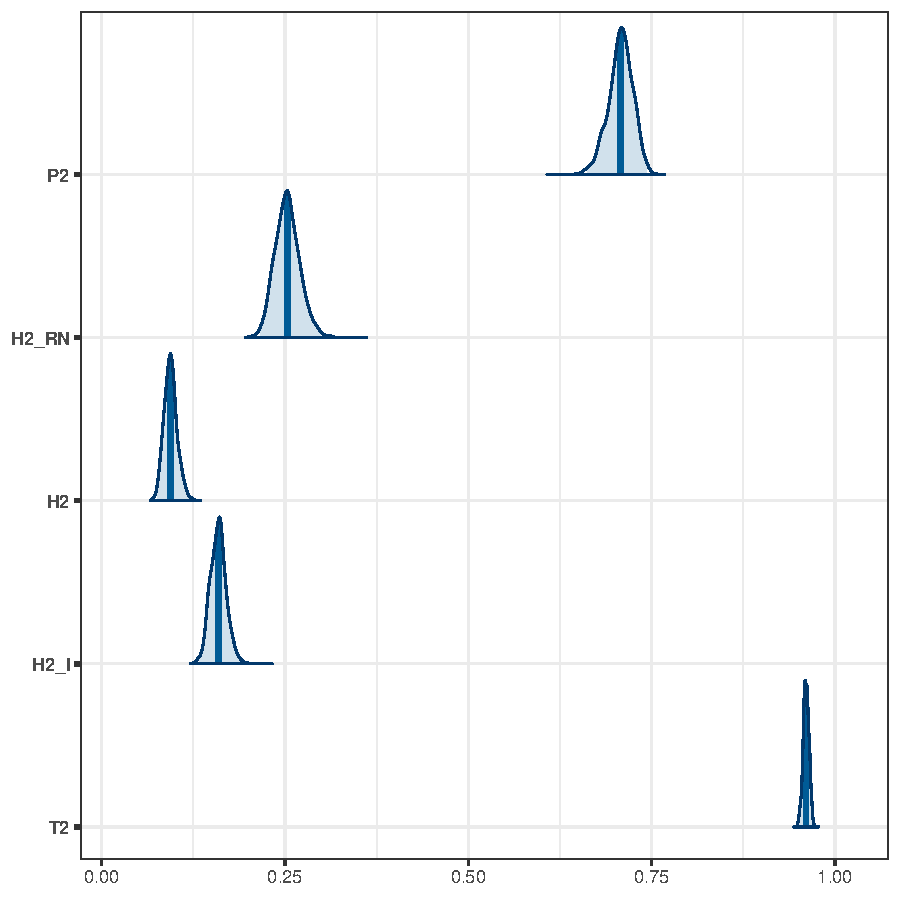
\includegraphics[width = 0.49\textwidth]{TPC_varstd_cs_ds.pdf}
  \caption{Posterior distribution of the variance-standardised estimates of our variance decomposition of the reaction norm of thermal performance, based on a character-state model.}
  \label{fig_tpc_cs_var_decomp_ds}
\end{figure}

\subsubsection{A better variance decomposition, combining quadratic and character-state models}

\paragraph{Studying the average reaction norm}
Since we know the variances obtained from the character-state model are more trustworthy, we can use them for our variance decomposition. But at the same time, we would still like to be able to say how much of the variation we observe is explained by a first-order linear trend or a second-order one.
To approximate such values, we can combine the estimates from the quadratic model with the variances (here $V_{\text{Plas}}$) obtained from the character-state model:
\begin{Rinput}
post_plas_tpc_withcs <-
    # Note that we get theta from the quadratic model,
    # but V_Plas from the character-state one
    map2(post_tpc[["Theta"]], post_cs[["V_Plas"]],
         \§§(th_, v_) rn_phi_decomp(theta   = th_,
                                   X      = design_mat,
                                   S      = S_theta_tpc,
                                   v_plas = v_),
         .progress = TRUE) |>
    bind_rows()  |>
    select(where(\§§(col_) { abs(mean(col_)) > 10^-5 })) |>
    cbind(post_tpc_info) |>
    as_draws_df()

summarise_draws(post_plas_tpc_withcs)
mcmc_trace(post_plas_tpc_withcs)
mcmc_areas(post_plas_tpc_withcs,
           regex_pars = "^V",
           prob = 0.95,
           area_method = "scaled height") /
    mcmc_areas(post_plas_tpc_withcs,
               regex_pars = "^[^V]",
               prob = 0.95,
               area_method = "scaled height") +
    plot_layout(heights = c(1, 3))
\end{Rinput}
\begin{Routput}
# A tibble: 4 × 10
  variable  mean median      sd     mad    q5   q95  rhat ess_bulk ess_tail
  <chr>    <dbl>  <dbl>   <dbl>   <dbl> <dbl> <dbl> <dbl>    <dbl>    <dbl>
1 V_Plas   0.136  0.136 0.00841 0.00838 0.122 0.150 1.00      886.    1051.
2 Phi_b    0.186  0.185 0.0287  0.0286  0.141 0.237 1.00      989.     916.
3 Phi_c    0.456  0.454 0.0487  0.0473  0.380 0.538 0.998    1004.    1016.
4 M2       0.642  0.638 0.0622  0.0624  0.541 0.748 1.00     1031.    1081.
\end{Routput}
This output (see also \autoref{fig_tpc_quadcs_var_decomp_ds}) is different from the one we obtained directly with the quadratic model. First, the value for $V_{\text{Plas}}$ (which was not computed here, but directly taken from \texttt{post\_cs}) is larger here.
Second, and a consequence, the values for $\varphi_{b}$ and $\varphi_{c}$ are smaller, and do not sum to 1 any more.
Of course, however, their relative values (i.e.\ $\varphi_{b}/\varphi_{c}$) is conserved.
Third, the function \texttt{rn\_phi\_decomp()} this time returned a new value: the ratio $M^{2}_{\text{Plas}}$ of the estimation of $V_{\text{Plas}}$ as estimated from the quadratic model to the estimation of $V_{\text{Plas}}$ from the character-state.
This value measures how well the quadratic model was a good approximation of the reaction norm.
Here, $M^{2}_{\text{Plas}} = 0.64$\footnote{Note that we were bad at all with our little computation above}, which is not extremely great (i.e.\ the fit is clearly not perfect and we should not have used the values from the quadratic model directly), but not too bad either (i.e.\ the combination with character-state as we're doing is still informative).
Note that, because the character-state does not make explicit assumptions about the shape of the reaction norm and is thus more ``encompassing'', we expect $M^{2}_{\text{Plas}} \leq 1$ in general.

\begin{figure}
  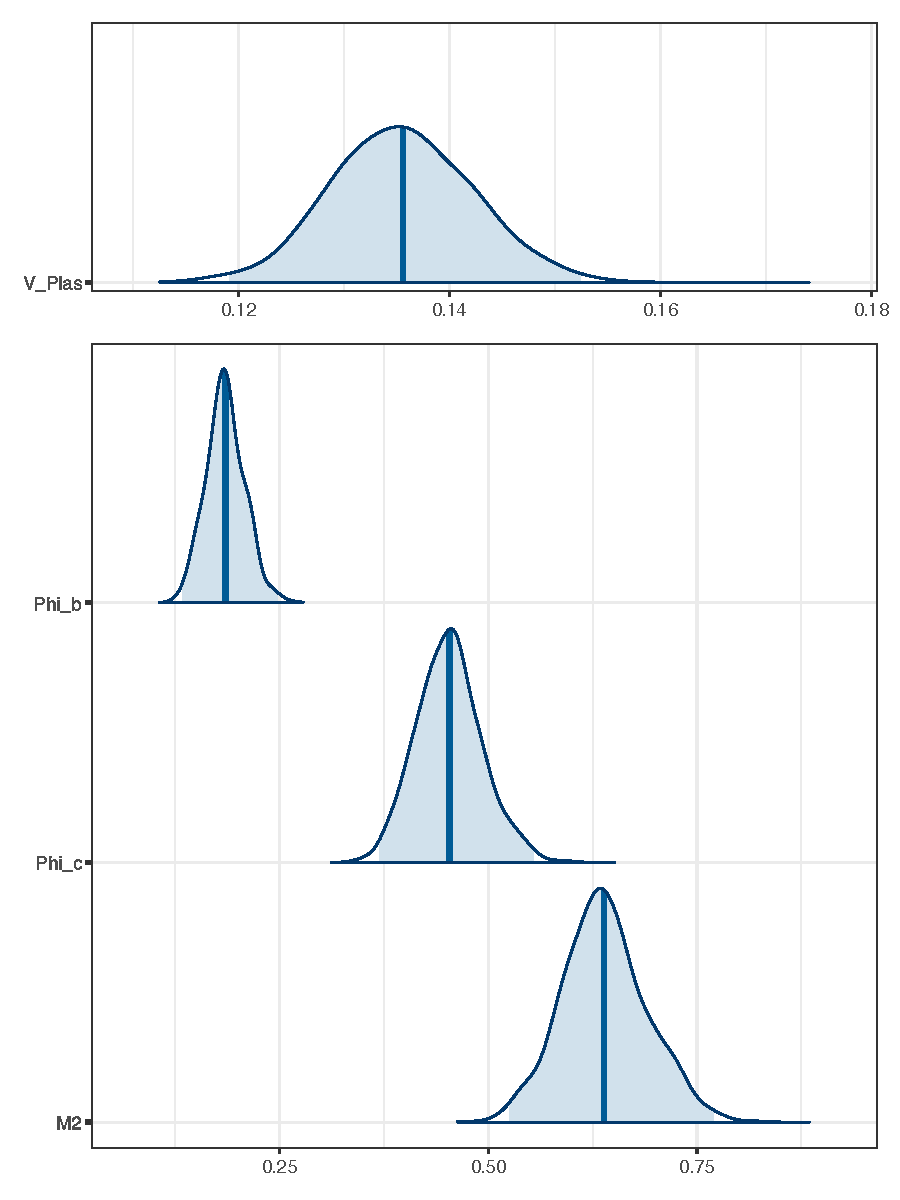
\includegraphics[width = 0.49\textwidth]{TPC_quadwithcs_plas_ds.pdf}
  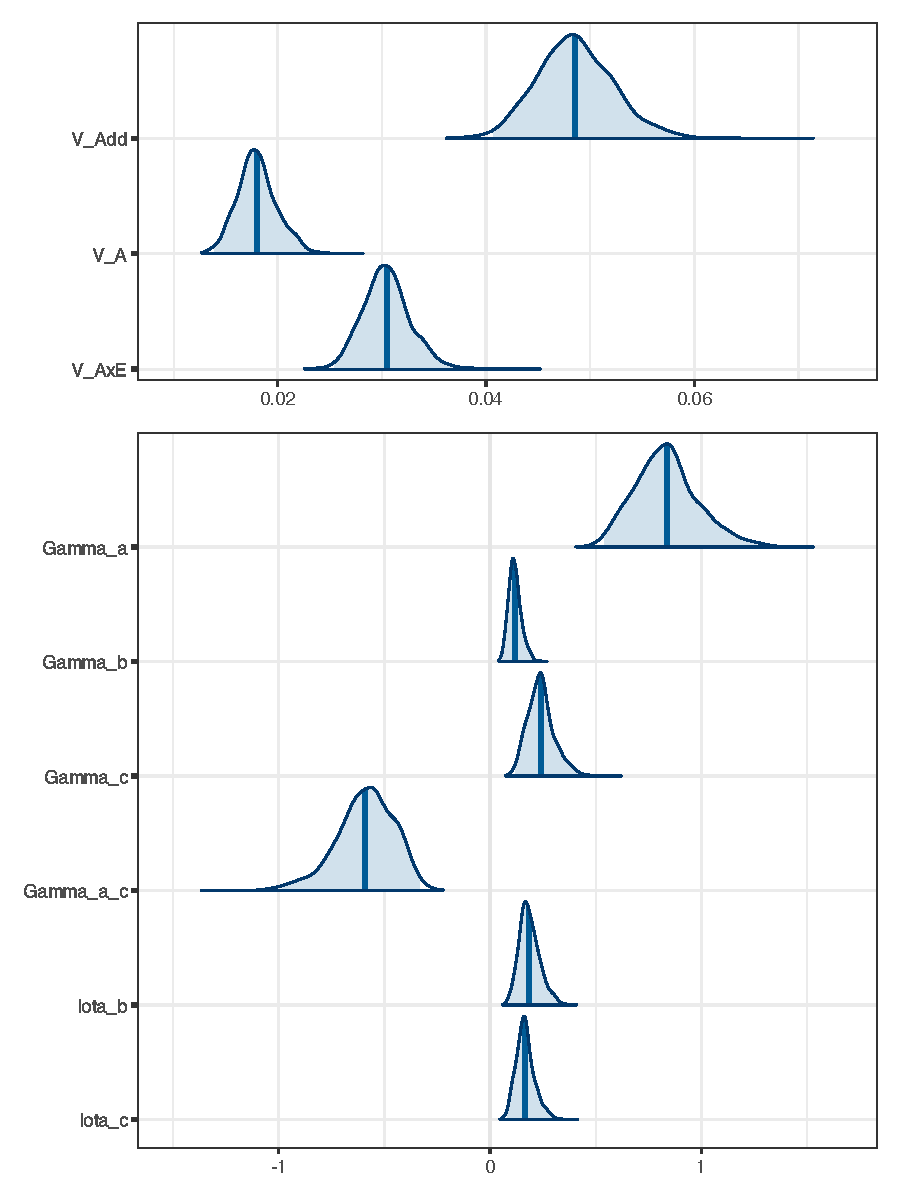
\includegraphics[width = 0.49\textwidth]{TPC_quadwithcs_gen_ds.pdf}
  \caption{Posterior distribution of the variance decomposition of the reaction norm of aggressiveness, based on a quadratic model.}
  \label{fig_tpc_quadcs_var_decomp_ds}
\end{figure}

\paragraph{Studying the additive genetic variation}
We can have the same hybrid approach to the additive genetic variance decomposition, by providing the parameters values from the quadratic model, but the estimated variances from the character-state. To do so, we will use the \texttt{add\_vars} argument from the \texttt{rn\_gen\_decomp()} function:
\begin{Rinput}
# Adding a column containing the three additive genetic variances
# to the character-state posterior draws
post_gen_cs[["Add_Vars"]] <-
    post_gen_cs |>
    select(starts_with("V")) |>
    apply(1, \§§(row_) { c(row_) }, simplify = FALSE)

# Calling rn_gen_decomp(), but provided values from the character-state
# to add_vars
post_gen_tpc_withcs <-
    pmap(list(th_ = post_tpc[["Theta"]],
              G_  = post_tpc[["G"]],
              v_  = post_gen_cs[["Add_Vars"]]),
         \§§(th_, G_, v_) rn_gen_decomp(theta    = th_,
                                      G_theta  = G_,
                                      X        = design_mat,
                                      add_vars = v_),
         .progress = TRUE) |>
    bind_rows()  |>
    select(where(\§§(col_) { abs(mean(col_)) > 10^-5 })) |>
    cbind(post_tpc_info) |>
    as_draws_df()

summarise_draws(post_gen_tpc_withcs)
mcmc_trace(post_gen_tpc_withcs)
mcmc_areas(post_gen_tpc_withcs,
           regex_pars = "^V",
           prob = 0.95,
           area_method = "scaled height") /
    mcmc_areas(post_gen_tpc_withcs,
               regex_pars = "^[^V]",
               prob = 0.95,
               area_method = "scaled height") +
    plot_layout(heights = c(3, 6))
\end{Rinput}
\begin{Routput}
# A tibble: 9 × 10
  variable     mean  median      sd     mad      q5     q95  rhat ess_bulk ess_tail
  <chr>       <dbl>   <dbl>   <dbl>   <dbl>   <dbl>   <dbl> <dbl>    <dbl>    <dbl>
1 V_Add      0.0488  0.0485 0.00461 0.00444  0.0419  0.0567  1.00     959.     949.
2 V_A        0.0182  0.0180 0.00235 0.00225  0.0146  0.0222  1.00    1011.     968.
3 V_AxE      0.0306  0.0305 0.00291 0.00265  0.0262  0.0356  1.00     922.     742.
4 Gamma_a    0.852   0.837  0.185   0.177    0.582   1.19    1.00     944.     913.
5 Gamma_b    0.121   0.118  0.0372  0.0358   0.0669  0.190   1.00     922.     888.
6 Gamma_c    0.249   0.240  0.0789  0.0736   0.136   0.392   1.00    1058.     993.
7 Gamma_a_c -0.607  -0.591  0.168   0.164   -0.917  -0.367   1.00    1004.     969.
8 Iota_b     0.193   0.185  0.0597  0.0562   0.106   0.305   1.00     946.     861.
9 Iota_c     0.173   0.167  0.0554  0.0516   0.0955  0.276   1.00    1039.     993.
\end{Routput}
See \autoref{fig_tpc_quadcs_var_decomp_ds} for the posterior distributions.
Of course, the values for $V_{\text{Add}}$, $V_{\text{A}}$ and $V_{\text{A}\times\text{E}}$ are the same as the one we computed from the character-state and, they were directly used and not re-computed.
Note also that, because we used the variances from the character-state to scale them (as we did for $\varphi$ above), the $\gamma$'s and $\iota$'s do not sum to 1 either in this case.
All of this is a bit ``hacky'' and not as good as finding a proper curve, fitting well our reaction norm, as we will see now.

\subsection{Analysing a reaction norm with a non-linear model}

\subsubsection{Running a non-linear model}
\label{subsubsec_nl_mod_ds}

\paragraph{The Gaussian-Gompertz function}
Looking at \autoref{fig_tpc_rn_plain}, the shape seems to follow the typical asymmetrical quasi-bell shape of thermal performance traits.
A commonly used function to study such kind of traits is the Gaussian-Gompertz function. It is a relatively complex function that depends on 4 parameters (highlighted below):
\begin{equation}
  \label{eq_gg}
  \hat{z} = \textcolor{purple}{C_{\text{max}}} 
  \exp\left(-\exp\left(\textcolor{purple}{\rho} \left(\varepsilon - \textcolor{purple}{\varepsilon_{0}}\right) - 6\right) -  \textcolor{purple}{\sigma} \left(\varepsilon - \textcolor{purple}{\varepsilon_{0}}\right)^2\right)
\end{equation}
However, for the sake of simplicity, we will only make two of them ($C_{\text{max}}$ and $\varepsilon_{0}$) vary genetically\footnote{If you are curious at to what it looks like in practice, you can spoil the end for yourself and look directly at \autoref{fig_pred_tpc_nl}.}.

\paragraph{Preparing the model}
Running a non-linear model in \texttt{brms} is relatively straightforward, but it does require new elements of syntax:
\begin{Rinput}
form_nl <- brmsformula(Performance ~ cmax * exp(
                                        - exp(rho * (Temp - xopt) - 6) -       # Gompertz part
                                            sigmagaus * (Temp - xopt)^2        # Gaussian part
                                    ),
                        cmax + xopt ~ 1 + (1 | ID1 | Individual),
                        rho + sigmagaus ~ 1,
                        nl = TRUE)
\end{Rinput}
Starting from the end, notice we set the argument \texttt{nl} to \texttt{TRUE}, telling \texttt{brmsformula()} that we want to set up a non-linear model. Then (still from the end), we set up two groups of parameters: \texttt{rho} and \texttt{sigmagaus} will be inferred, but fixed across individuals; while \texttt{cmax} and \texttt{xopt} will be allow to vary across individuals.
The \texttt{ID1} part is just a placeholder (it could be any string of character) to tell \texttt{brms} that we want to infer the covariances between \texttt{cmax} and \texttt{xopt}.
Finally (at the top), we define the equation of the model, linking the response variable \texttt{Performance} with the environmental variable \texttt{Temp}, following \autoref{eq_gg}.
While we were using the default priors until now, the situation is different for a non-linear model, because it is hard for \texttt{brms} to come up with relevant priors for the non-linear parameters.
So, we will help it by providing priors for the parameters that cannot take negative values. 
Although we could come up with smarter priors, we will simply here use uniform priors for those parameters, specifying a higher bound far away enough from the values that we expect to be realistic:
\begin{Rinput}
prior_nl <- 
    prior(uniform(0, 10), nlpar = "cmax", lb = 0, ub = 100) +
    prior(uniform(0, 100), nlpar = "rho", lb = 0, ub = 100) +
    prior(uniform(0, 10), nlpar = "sigmagaus", lb = 0, ub = 10)
\end{Rinput}
Another thing that is now required and that is difficult for \texttt{brms} to figure out are the starting values for the non-linear parameters, which we will thus provide based on ballpark idea of what their value should be:
\begin{Rinput}
inits <- rep(list(list(b_cmax      = array(data = 1),
                        b_xopt      = array(data = 0.9),
                        b_rho       = array(data = 8),
                        b_sigmagaus = array(data = 0.4))), 4)
\end{Rinput}
Finally, we will use an increased total number of iterations:
\begin{Rinput}
# Total number of iterations
n_iter_nl <- 7000
# Number of iterations that will be discarded for the warm-up
n_warm_nl <- 1000
# Thinning interval
n_thin_nl <- 1
\end{Rinput}
Now, we are ready to run the model!

\paragraph{Running the model}
Now that we have prepared everything, running the model is very much like the linear instance (although note that we now provide \texttt{prior} and \texttt{init}):
\begin{Rinput}
model_nl_tpc <-
    brm(formula   = form_nl,
        data      = tbl_dragon_ds,
        save_pars = save_pars(group = FALSE),
        chains    = n_chains,
        cores     = n_chains,
        seed      = seed,
        init      = inits,
        prior     = prior_nl,
        iter      = n_iter_nl,
        warmup    = n_warm_nl,
        thin      = n_thin_nl)
\end{Rinput}
This might take a bit longer than the other models, but not by much.

\paragraph{Checking the model}
Let's look at the model estimates:
\begin{Rinput}
summary(model_nl_tpc)
\end{Rinput}
\begin{Routput}
 Family: gaussian 
  Links: mu = identity; sigma = identity 
Formula: Performance ~ cmax * exp(-exp(rho * (Temp - xopt) - 6) - sigmagaus * (Temp - xopt)^2) 
         cmax ~ 1 + (1 | ID1 | Individual)
         xopt ~ 1 + (1 | ID1 | Individual)
         rho ~ 1
         sigmagaus ~ 1
   Data: tbl_dragon_ds (Number of observations: 1000) 
  Draws: 4 chains, each with iter = 7000; warmup = 1000; thin = 1;
         total post-warmup draws = 24000

Multilevel Hyperparameters:
~Individual (Number of levels: 100) 
                                   Estimate Est.Error l-95% CI u-95% CI Rhat Bulk_ESS Tail_ESS
sd(cmax_Intercept)                     0.32      0.02     0.28     0.38 1.00     1777     3667
sd(xopt_Intercept)                     0.21      0.02     0.18     0.24 1.00     2524     5804
cor(cmax_Intercept,xopt_Intercept)     0.24      0.10     0.02     0.43 1.00     1459     2915

Regression Coefficients:
                    Estimate Est.Error l-95% CI u-95% CI Rhat Bulk_ESS Tail_ESS
cmax_Intercept          1.01      0.03     0.95     1.08 1.01      813     1833
xopt_Intercept          0.95      0.03     0.90     1.01 1.00     1994     5184
rho_Intercept           8.37      0.27     7.88     8.93 1.00     9192    13020
sigmagaus_Intercept     0.38      0.01     0.36     0.40 1.00    10942    14635

Further Distributional Parameters:
      Estimate Est.Error l-95% CI u-95% CI Rhat Bulk_ESS Tail_ESS
sigma     0.10      0.00     0.10     0.11 1.00    18600    18545

Draws were sampled using sampling(NUTS). For each parameter, Bulk_ESS
and Tail_ESS are effective sample size measures, and Rhat is the potential
scale reduction factor on split chains (at convergence, Rhat = 1).
\end{Routput}
The $\hat{R}$ and effective sample size for all parameters are acceptable, and the point values and credible intervals for them seem coherent. We can verify also graphically that everything went smoothly by looking at their trace and posterior distributions (see \autoref{fig_mod_tpc_nl}):
\begin{Rinput}
plot(model_nl_tpc)
\end{Rinput}
%
\begin{figure}[t!h!]
  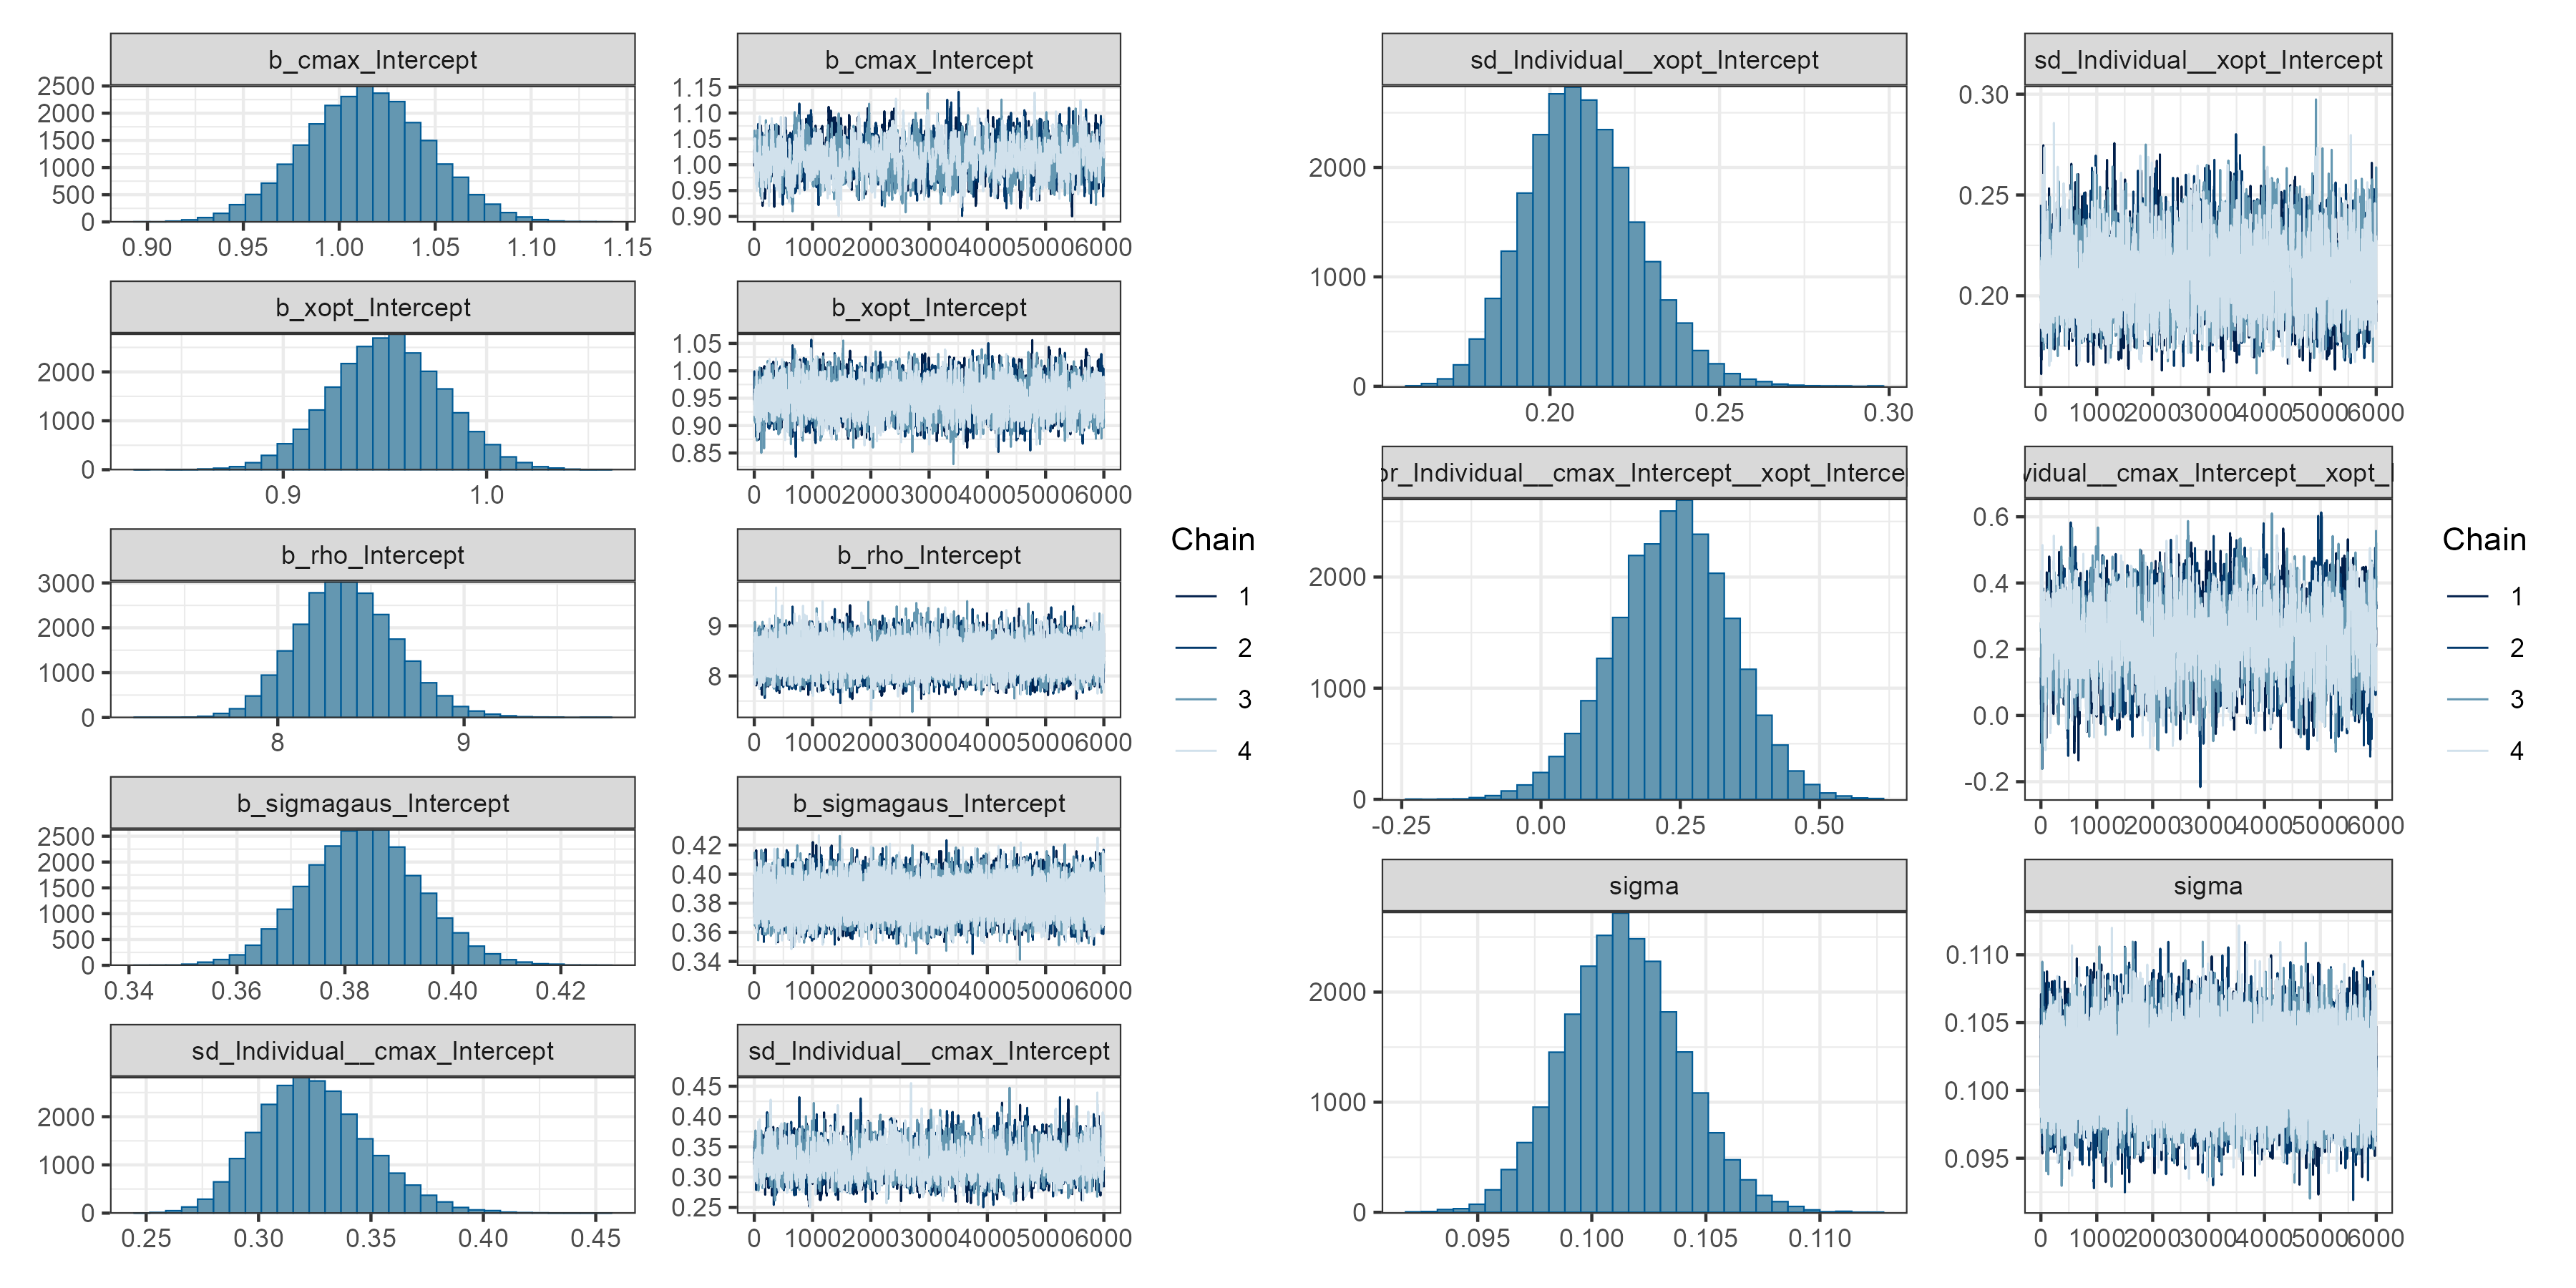
\includegraphics[width = \textwidth]{TPC_nl_model_ds.png}
  \caption{Plot of the \texttt{mod\_nl\_tpc} model. Parameters starting with ``b'' are the fixed effects of the non-linear parameters of the model, and parameters starting with ``sd'' are the standard deviation of the random effects of the non-linear parameters. The parameter ``sigma'' is the residual standard deviation.}
  \label{fig_mod_tpc_nl}
\end{figure}
%
Finally, we can also look at the fit of the model to the raw data, by placing the model predictions over the raw phenotypes (see \autoref{fig_pred_tpc_nl}):
\begin{Rinput}
tbl_tpc_mod <-
    tbl_dragon_ds |>
    mutate(Predict = predict(model_nl_tpc, re_formula = NA) |>
                     as_tibble()) |>
    unpack(Predict) |>
    select(Temp,
           Predict = Estimate,
           Predict_Low = Q2.5,
           Predict_Up  = Q97.5) |>
    summarise(across(starts_with("Predict"), mean),
              .by = Temp)

p_rn_tpc <-
    p_tpc +
    geom_ribbon(data = tbl_tpc_mod,
                mapping = aes(x = Temp, ymin = Predict_Low, ymax = Predict_Up),
                alpha = 0.3) +
    geom_line(data = tbl_tpc_mod,
              mapping = aes(x = Temp, y = Predict),
              linewidth = 1)
\end{Rinput}
%
\begin{figure}[h!]
  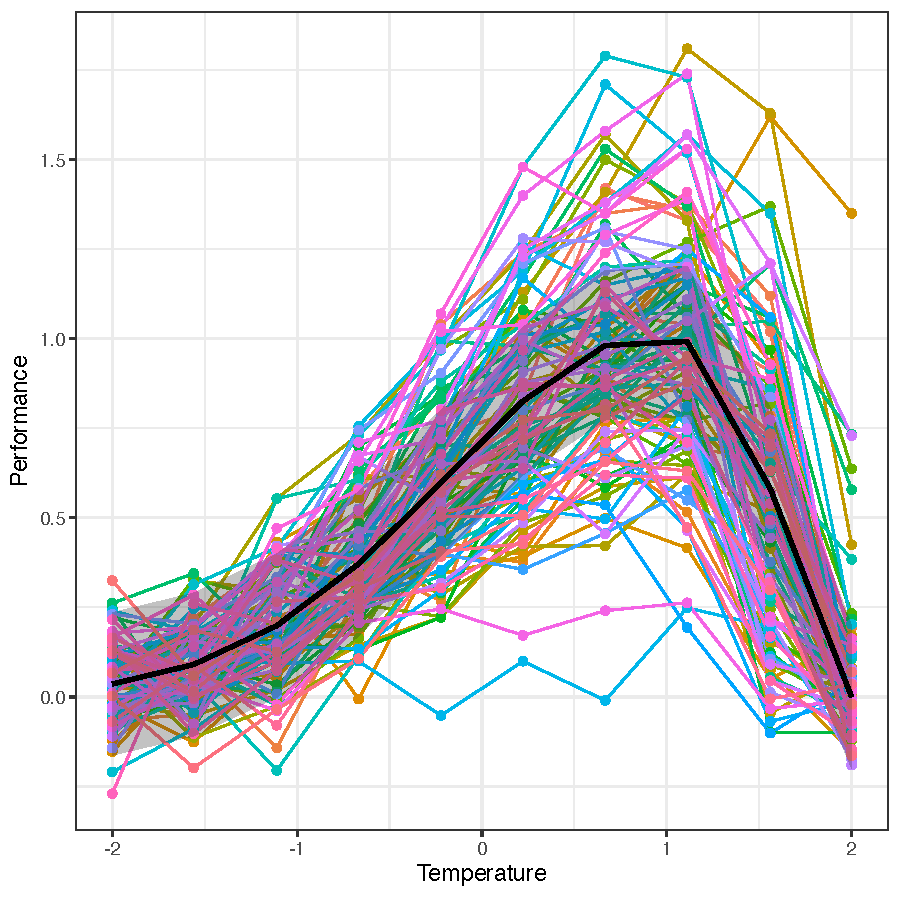
\includegraphics[width = 0.7\textwidth]{TPC_discrete_nonlinear_pred.pdf}
  \caption{Thermal performance individual data, with the non-linear reaction norm predicted by the \texttt{mod\_tpc\_nl} model.}
  \label{fig_pred_tpc_nl}
\end{figure}
The fit this time is much better than with the quadratic curve\footnote{Well, that is to be expected, because this happen to be exactly the true curve of reaction norms.}. So, with this much better curve, we should be able to readily apply our variance decomposition!

\subsubsection{Decomposing the variance of a non-linear model}

\paragraph{Extracting the parameters}
The code used to extract the estimation of the parameters of interest for the variance decomposition is surprisingly similar to the linear case.
We just to do a bit more work regarding the names:
\begin{Rinput}
theta_post_nl_tpc <- fixef(model_nl_tpc, summary = FALSE)
# We remove the "_Intercept" part of the name
colnames(theta_post_nl_tpc) <- str_remove(colnames(theta_post_nl_tpc), "_Intercept")
head(theta_post_nl_tpc)
\end{Rinput}
\begin{Routput}
    variable
draw      cmax      xopt      rho sigmagaus
   1 0.9968932 0.9641778 8.219535 0.3843630
   2 1.0087171 0.9462906 8.454820 0.3873613
   3 1.0038337 0.9577721 8.381722 0.3799357
   4 1.0123249 0.9456947 8.433239 0.3816431
   5 0.9988809 0.9244892 8.479489 0.3733265
   6 1.0398035 0.9162629 8.312176 0.3971904
\end{Routput}
\begin{Rinput}
G_post_nl_tpc <-
    VarCorr(model_nl_tpc, summary = FALSE)[["Individual"]][["cov"]] |>
    apply(1, \§§(mat_) { mat_ }, simplify = FALSE) |>
    # Same here for "_Intercept" part of the name
    map(\§§(mat_) { rownames(mat_) <- colnames(mat_) <- str_remove(rownames(mat_), "_Intercept"); return(mat_) })
G_post_nl_tpc[[1]]
\end{Rinput}
\begin{Routput}
            cmax        xopt
cmax 0.102789698 0.001781295
xopt 0.001781295 0.028796905
\end{Routput}
\begin{Rinput}
vr_post_nl_tpc <-
    VarCorr(model_nl_tpc, summary = FALSE)[["residual__"]][["sd"]][ , 1]^2
\end{Rinput}
The object \texttt{theta\_post\_nl\_tpc} contains all the ``fixed effect'' part of the parameters estimation, while \texttt{G\_post\_nl\_tpc} contains the variances and covariance estimates from their ``random part''.
Remember that we only allowed \texttt{cmax} and \texttt{xopt} to vary genetically across individuals in the model.
Because of that, our $\mathbf{G}$-matrix is smaller than our parameter vector $\bar{\theta}$, but worry not, as \texttt{Reacnorm} will be able to account for this!
It is especially important here to reduce the number of kept iterations to a thousand, because the functions that we will use rely (more) on numerical integration and are thus a bit slower:
\begin{Rinput}
post_nl_tpc <- as_draws_df(theta_post_nl_tpc)
post_nl_tpc[["G"]] <- G_post_nl_tpc
post_tpc[["Theta"]] <-
    post_tpc |>
    select(a:c) |>
    apply(1, \§§(vec_) { vec_ }, simplify = FALSE)
post_nl_tpc[["V_R"]] <- vr_post_nl_tpc
post_nl_tpc <- thin_draws(post_nl_tpc, thin = nrow(theta_post_nl_tpc) / 1000)
# Keep the iteration/chain info to create new posterior objects
post_nl_tpc_info <- select(post_nl_tpc, starts_with("."))
\end{Rinput}

\paragraph{Generating the expression for the reaction norm curve}
Because the model in non-linear this time, \texttt{Reacnorm} has no idea what the assumed shape of the reaction norm was simply based on vector of parameters and the environmental values (i.e.\ the \texttt{design\_matrix} we used before).
This time, we need to be able to provide the functions with the shape we used for the reaction norm.
To do so, we will have to generate an ``expression'' in R, which will refer to the environment as \texttt{x} and use \textbf{exactly the same parameter names as we did for \texttt{brms}}.
This can be done quite easily in R using the \texttt{expression()} function:
\begin{Rinput}
gg_shape <- expression(
    cmax * exp(
        - exp(rho * (x - xopt) - 6) -
            sigmagaus * (x - xopt)^2
    )
)
\end{Rinput}
We will also require a vector of unique environmental value that we will prepare:
\begin{Rinput}
vec_env <- unique(tbl_dragon_ds[["Temp"]])
\end{Rinput}

\paragraph{Computing the variance of average reaction norm (and its decomposition?)}
This time, since the model is non-linear, we cannot compute the $\varphi$-decomposition using the \texttt{rn\_phi\_decomp()}.
Also, because the environmental variable is a fixed, discretised variable, it does not follow a normal distribution, so we cannot properly compute the $\pi$-decomposition either\footnote{Although we'll see how we can find a way in an instant}.
Still, we can obtain $V_{\text{Plas}}$ directly using the \texttt{rn\_vplas()} function. To do so, we have to provide the shape of the reaction norm (with \texttt{gg\_shape}) and the vector of environmental values (with \texttt{vec\_env}) directly.
Finally, we need to state to \texttt{Reacnorm} that the third (\texttt{rho}) and fourth (\texttt{sigmagaus}) values of the vector of parameters are not present in the $\mathbf{G}$-matrix, which we do using the \texttt{fixed} parameter:
\begin{Rinput}
post_v_plas_nl_tpc <-
    map2(post_nl_tpc[["Theta"]], post_nl_tpc[["G"]],
         \§§(th_, G_) { data.frame(V_Plas = rn_vplas(theta    = th_,
                                                   G_theta  = G_,
                                                   env      = vec_env,
                                                   shape    = gg_shape,
                                                   fixed    = c(3, 4))) },
         .progress = TRUE) |>
    bind_rows() |>
    cbind(post_nl_tpc_info) |>
    as_draws_df()
summarise_draws(post_v_plas_nl_tpc)
\end{Rinput}
\begin{Routput}
# A tibble: 1 × 10
  variable  mean median      sd     mad    q5   q95  rhat ess_bulk ess_tail
  <chr>    <dbl>  <dbl>   <dbl>   <dbl> <dbl> <dbl> <dbl>    <dbl>    <dbl>
1 V_Plas   0.121  0.121 0.00801 0.00791 0.108 0.135  1.01     763.     689.
\end{Routput}
Note that this value is relatively close to the one we obtained using the character-state model in \autoref{subsubsec_tpc_cs}.

\paragraph{The $\pi$-decomposition assuming a normal distribution}
Now, if we wanted to still use the $\pi$-decomposition, we would need to assumed that the temperature is actually normally distributed.
One way to do so is to weight each of the environments according the density of a normal distribution.
We can use the \texttt{dnorm()} function to compute such densities and pass them to \texttt{wt\_env} argument of \texttt{Reacnorm}.
This way, we can use the \texttt{rn\_pi\_decomp()} function of \texttt{Reacnorm}, since we're assuming a normal distribution:
\begin{Rinput}
post_plas_nl_tpc_norm <-
    map2(post_nl_tpc[["Theta"]], post_nl_tpc[["G"]],
         \§§(th_, G_) { rn_pi_decomp(theta    = th_,
                                   G_theta  = G_,
                                   env      = vec_env,
                                   shape    = gg_shape,
                                   fixed    = c(3, 4),
                                   wt_env   = dnorm(vec_env)) },
         .progress = TRUE) |>
    bind_rows() |>
    cbind(post_nl_tpc_info) |>
    as_draws_df()
summarise_draws(post_plas_nl_tpc_norm)
\end{Rinput}
\begin{Routput}
# A tibble: 3 × 10
  variable   mean median      sd     mad     q5   q95  rhat ess_bulk ess_tail
  <chr>     <dbl>  <dbl>   <dbl>   <dbl>  <dbl> <dbl> <dbl>    <dbl>    <dbl>
1 V_Plas   0.0927 0.0927 0.00621 0.00619 0.0828 0.103 1.01      761.     755.
2 Pi_Sl    0.329  0.325  0.0265  0.0205  0.292  0.384 0.998     818.     953.
3 Pi_Cv    0.195  0.195  0.0101  0.00949 0.178  0.211 0.999     871.    1032.
\end{Routput}
Since we assumed a different distribution for the environment, the estimated value for $V_{\text{Plas}}$ changed.
This time, however, we obtained a proper $\pi$-decomposition into a slope and curvature components\footnote{Note that we could have used the same trick for the quadratic curve we used above, but given the not-so-good fit, the results would not have been very trustworthy.}.
Notably, the part of the variance arising from the slope is considerable ($\pi_{\text{Sl}} = 0.33$), as is the part arising from curvature to a lesser extent ($\pi_{\text{Cv}} = 0.20$).
It should be noted, for the interpretation of those values, that since we assumed a normal distribution, the values of the environment close to 0 (the mean value of the environment) are given more weight than values close to -2 or 2.
As such, the slope and curvature near 0 are the ones that are driving the values for $\pi_{\text{Sl}}$ and $\pi_{\text{Cv}}$.

\paragraph{Computing the additive genetic variance decomposition}
When studying the additive genetic variance, we do not require the normality assumption about the environment to perform the $\gamma$- or $\iota$-decomposition, and thus, we can readily apply the \texttt{rn\_gen\_decomp()} function:
\begin{Rinput}
post_gen_nl_tpc <-
    map2(post_nl_tpc[["Theta"]], post_nl_tpc[["G"]],
         \§§(th_, G_) { rn_gen_decomp(theta    = th_,
                                    G_theta  = G_,
                                    env      = vec_env,
                                    shape    = gg_shape,
                                    fixed    = c(3, 4)) },
         .progress = TRUE) |>
    bind_rows() |>
    select(where(\§§(col_) { abs(mean(col_)) > 10^-5 })) |>
    cbind(post_nl_tpc_info) |>
    as_draws_df()
summarise_draws(post_gen_nl_tpc)
\end{Rinput}
\begin{Routput}
# A tibble: 9 × 10
  variable            mean   median      sd     mad       q5       q95  rhat ess_bulk ess_tail
  <chr>              <dbl>    <dbl>   <dbl>   <dbl>    <dbl>     <dbl> <dbl>    <dbl>    <dbl>
1 V_Add            0.0495   0.0491  0.00557 0.00552  0.0411   0.0594   1.01      994.     836.
2 V_A              0.0224   0.0220  0.00342 0.00355  0.0173   0.0284   1.01      936.     800.
3 V_AxE            0.0272   0.0271  0.00250 0.00251  0.0234   0.0314   1.01     1024.     984.
4 Gamma_cmax       0.700    0.703   0.0403  0.0412   0.632    0.762    1.00      864.     892.
5 Gamma_xopt       0.303    0.300   0.0405  0.0415   0.241    0.373    1.00      870.     893.
6 Gamma_cmax_xopt -0.00298 -0.00204 0.00327 0.00249 -0.00965  0.000270 0.999     811.     856.
7 Iota_cmax        0.460    0.461   0.0490  0.0509   0.382    0.540    1.00      873.     943.
8 Iota_xopt        0.548    0.548   0.0494  0.0509   0.469    0.629    1.00      881.     979.
9 Iota_cmax_xopt  -0.00806 -0.00638 0.00692 0.00588 -0.0214  -0.000332 1.00      834.     943.
\end{Routput}
Comparing such values with the character-state model in \autoref{subsubsec_tpc_cs}, the values for the total additive genetic variance ($V_{\text{Add}}$) are very close, but the values for $V_{\text{A}}$ and $V_{\text{A}\times\text{E}}$ are different, with more balance between these two components in this non-linear model than in the character-state model.
Given the credible intervals, this is likely to be just stochastic fluctuation.
As we can see, most of the additive genetic variance in the reaction norm seems to come from genetic variation in $C_{\text{max}}$ ($\gamma_{C_{\text{max}}} = 0.7$), while the (short) majority of the additive genetic variation in plasticity rather comes from $\varepsilon_{0}$ ($\iota_{\varepsilon_{0}} = 0.55$).
Since the model is non-linear this time, there is a distinction to be made between $V_{\text{Add}}$ and $V_{\text{Gen}}$ which are not equal any more.
So, we can compute $V_{\text{Gen}}$ separately:
\begin{Rinput}
post_gen_nl_tpc[["V_Gen"]] <-
    map2_dbl(post_nl_tpc[["Theta"]], post_nl_tpc[["G"]],
             \§§(th_, G_) { rn_vgen(theta    = th_,
                                  G_theta  = G_,
                                  env      = vec_env,
                                  shape    = gg_shape,
                                  fixed    = c(3, 4)) },
             .progress = TRUE) 
summarise_draws(post_gen_nl_tpc)
\end{Rinput}
\begin{Routput}
# A tibble: 10 × 10
   variable       mean   median      sd     mad       q5      q95  rhat ess_bulk
   <chr>         <dbl>    <dbl>   <dbl>   <dbl>    <dbl>    <dbl> <dbl>    <dbl>
 1 V_Add       0.0495   0.0491  0.00557 0.00552  0.0411   5.94e-2 1.01      994.
 2 V_A         0.0224   0.0220  0.00342 0.00355  0.0173   2.84e-2 1.01      936.
 3 V_AxE       0.0272   0.0271  0.00250 0.00251  0.0234   3.14e-2 1.01     1024.
 4 Gamma_cmax  0.700    0.703   0.0403  0.0412   0.632    7.62e-1 1.00      864.
 5 Gamma_xopt  0.303    0.300   0.0405  0.0415   0.241    3.73e-1 1.00      870.
 6 Gamma_cma… -0.00298 -0.00204 0.00327 0.00249 -0.00965  2.70e-4 0.999     811.
 7 Iota_cmax   0.460    0.461   0.0490  0.0509   0.382    5.40e-1 1.00      873.
 8 Iota_xopt   0.548    0.548   0.0494  0.0509   0.469    6.29e-1 1.00      881.
 9 Iota_cmax… -0.00806 -0.00638 0.00692 0.00588 -0.0214  -3.32e-4 1.00      834.
10 V_Gen       0.0579   0.0531  0.0417  0.00626  0.0444   6.58e-2 1.01     1017.
# ℹ 1 more variable: ess_tail <dbl>
\end{Routput}
We can see that $V_{\text{Gen}}$ is slightly higher than $V_{\text{Add}}$, because the non-linearity in the model is introducing non-additive genetic variance in the trait, even though all the genetic variance in the parameters is additive.

\paragraph{Computing the additive genetic variance decomposition with a normal assumption}
If we wanted to match the $\pi$-decomposition assuming a normal distribution, we can also compute the $\gamma$- and $\iota$-decomposition also assuming a normal distribution, using the same \texttt{wt\_env} argument\footnote{Notet that we have to set the argument \textit{width} to 8 here, due to a slight numerical instability when it is set to 10. It is not advisable to reduce this argument too much beyond that limit, as this will start to generate underestimation of the variance.}:
\begin{Rinput}
post_gen_nl_tpc_norm <-
    map2(post_nl_tpc[["Theta"]], post_nl_tpc[["G"]],
         \§§(th_, G_) { rn_gen_decomp(theta    = th_,
                                    G_theta  = G_,
                                    env      = vec_env,
                                    shape    = gg_shape,
                                    fixed    = c(3, 4),
                                    wt_env   = dnorm(vec_env),
                                    width    = 8) },
         .progress = TRUE) |>
    bind_rows() |>
    select(where(\§§(col_) { abs(mean(col_)) > 10^-5 })) |>
    cbind(post_nl_tpc_info) |>
    as_draws_df()

summarise_draws(post_gen_nl_tpc_norm)
\end{Rinput}
\begin{Routput}
# A tibble: 9 × 10
  variable        mean   median      sd     mad       q5      q95  rhat ess_bulk
  <chr>          <dbl>    <dbl>   <dbl>   <dbl>    <dbl>    <dbl> <dbl>    <dbl>
1 V_Add        0.0547   0.0540  0.00684 0.00670  0.0442   0.0668  1.01      931.
2 V_A          0.0349   0.0345  0.00536 0.00536  0.0269   0.0447  1.01      882.
3 V_AxE        0.0197   0.0197  0.00190 0.00191  0.0169   0.0231  1.01     1058.
4 Gamma_cmax   0.850    0.851   0.0406  0.0415   0.783    0.915   1.00      818.
5 Gamma_xopt   0.217    0.215   0.0354  0.0349   0.164    0.281   1.00      877.
6 Gamma_cmax… -0.0666  -0.0643  0.0330  0.0317  -0.125   -0.0133  0.998     798.
7 Iota_cmax    0.484    0.486   0.0498  0.0508   0.402    0.563   1.00      879.
8 Iota_xopt    0.513    0.512   0.0495  0.0501   0.434    0.595   1.00      883.
9 Iota_cmax_…  0.00271  0.00303 0.00273 0.00213 -0.00209  0.00622 1.00      932.
# ℹ 1 more variable: ess_tail <dbl>
\end{Routput}

\begin{figure}[b!]
  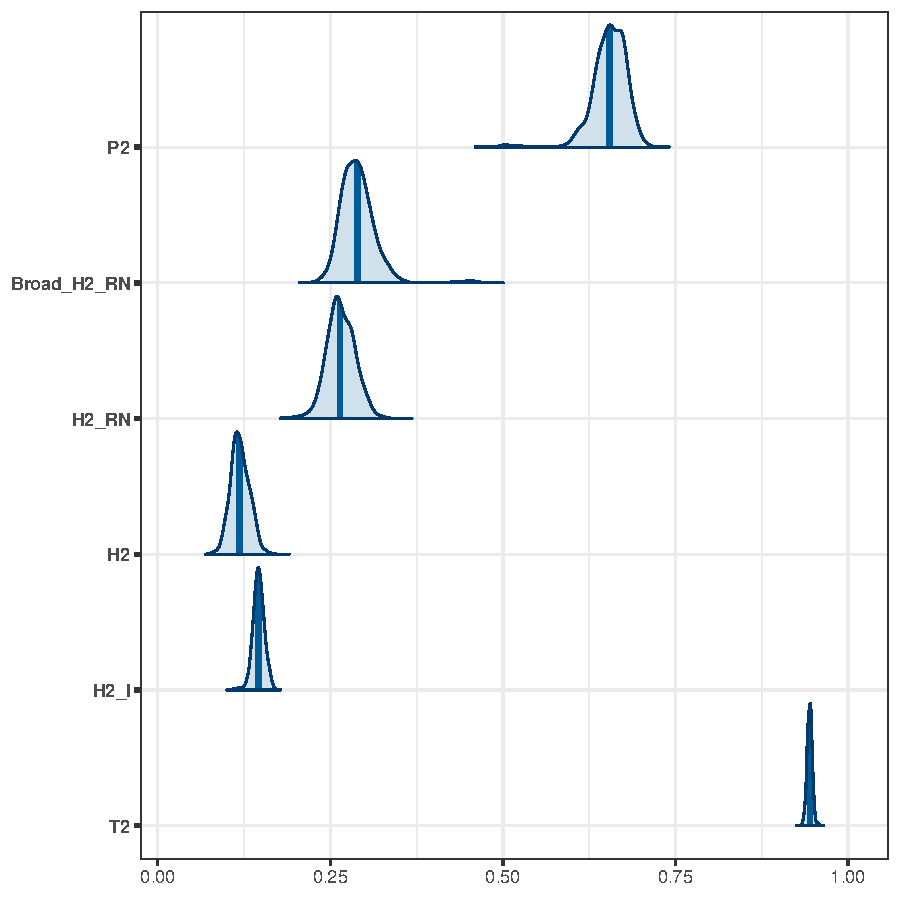
\includegraphics[width = 0.49\textwidth]{TPC_varstd_ds.pdf}
  \caption{Posterior distribution of the variance-standardised estimates of our variance decomposition of the reaction norm of thermal performance, based on the non-linear model.}
  \label{fig_tpc_nl_var_decomp_ds}
\end{figure}

\paragraph{Computing the variance-standardised estimates}
We have to gather all our estimates to compute the total phenotypic variance in the reaction norm, and use it to standardise our estimates.
This will be done almost exactly as for aggressiveness and the character-state of thermal performance (see \autoref{fig_tpc_nl_var_decomp_ds}), with the main difference being that we need to use $V_{\text{Gen}}$ rather than $V_{\text{Add}}$:
\begin{Rinput}
post_var_nl_tpc <-
    bind_draws(post_nl_tpc, post_v_plas_nl_tpc, post_gen_nl_tpc) |>
    subset_draws(variable = c("V_Plas", "V_Gen", "V_Add", "V_A", "V_AxE", "V_R")) |>
    mutate_variables(V_Tot = V_Plas + V_Gen + V_R)

post_std_nl_tpc <-
    post_var_nl_tpc |>
    transmute(P2            = V_Plas / V_Tot,
              Broad_H2_RN   = V_Gen / V_Tot,
              H2_RN         = V_Add / V_Tot,
              H2            = V_A / V_Tot,
              H2_I          = V_AxE / V_Tot,
              T2            = (V_Plas + V_Gen) / V_Tot) |>
    cbind(post_nl_tpc_info) |>
    as_draws_df()
    
summarise_draws(post_std_nl_tpc)
mcmc_trace(post_std_nl_tpc)
mcmc_areas(post_std_nl_tpc,
           prob = 0.95,
           area_method = "scaled height")
\end{Rinput}
\begin{Routput}
# A tibble: 6 × 10
  variable     mean median      sd     mad     q5   q95  rhat ess_bulk ess_tail
  <chr>       <dbl>  <dbl>   <dbl>   <dbl>  <dbl> <dbl> <dbl>    <dbl>    <dbl>
1 P2          0.648  0.654 0.0395  0.0278  0.586  0.694  1.01     948.     785.
2 Broad_H2_RN 0.297  0.289 0.0417  0.0283  0.250  0.363  1.01     976.     905.
3 H2_RN       0.265  0.264 0.0261  0.0250  0.223  0.307  1.01     796.     857.
4 H2          0.120  0.119 0.0167  0.0168  0.0935 0.147  1.01     790.     761.
5 H2_I        0.145  0.146 0.0115  0.00973 0.126  0.163  1.01     968.     982.
6 T2          0.945  0.945 0.00490 0.00457 0.937  0.953  1.00     972.     952.
\end{Routput}
So, most of the total variance is coming from the average shape of the reaction norm ($P^{2}_{\text{RN}} = 0.65$), and less from the total genetic variation ($H^{2}_{\text{RN}} = 0.30$).
Regarding, more specifically, the additive genetic variation ($h^{2}_{\text{RN}} = 0.27$), it composed of almost the same amount of marginal heritability of the trait ($h^{2}=0.12$) and heritability of plasticity ($h^{2}_{\text{I}} = 0.15$).
As for the character-state, the reaction norm explains almost all of the total phenotypic variation ($T^{2}_{\text{RN}}=0.95$).


\section{Studying reaction norms in a continuous environment}

In this section, we will now assume that phenotypic measurements are performed in a wild population of dragons, with heterogeneous micro-environements, especially temperature.
Because individuals move around this environment, it is possible to measure the same individual multiple times, but at different environmental values.

\subsection{A quadratic reaction norm}

\subsubsection{Data on aggressiveness}

Let's look at the data that are shipped with the \texttt{Reacnorm} package:
\begin{Rinput}
head(dragon_continuous)
\end{Rinput}
\begin{Routput}
  Individual Family   Temp Aggressiveness Performance
1    Ind_001  Fam_1  0.982          2.190       1.080
2    Ind_001  Fam_1  0.469          2.060       1.290
3    Ind_001  Fam_1 -0.108          1.660       0.868
4    Ind_001  Fam_1 -0.213          1.290       0.786
5    Ind_001  Fam_1  1.160          0.698       1.280
6    Ind_001  Fam_1  1.290          1.180       0.980
\end{Routput}
We have several measurements on individuals, at different measured temperatures (standardised to a mean of 0 and a variance of 1), as well as the family they belong to. Since dragons have a promiscuous reproduction, it can be assumed that all dragons from the same family are half-sibs (i.e.\ same mother, different father), with no shared paternity across families (this is a very large population of dragons).

To get to the additive genetic variance of the parameters, we will thus use a relatedness matrix based on such information matrix. For this, we will require the \texttt{Matrix} package to construct a block-diagonal matrix of 0.25 relatedness within families:
\begin{Rinput}
library(Matrix)
A_fam <- matrix(0.25, ncol = 10, nrow = 10) + 0.75 * diag(10)
A <- bdiag(rep(list(A_fam), 10))
colnames(A) <- rownames(A) <- sprintf("Ind_%03d", 1:100)
\end{Rinput}

Let's look a bit closer a the Aggressiveness column. It contains again a measure of aggressiveness when dragons are exposed to an armoured knight, but this time in the field\footnote{Knights are protected within a cage and have their armour, no knight was harmed during the protocol, which was validated by an ethics committee.}. We can plot its relation with temperature:
\begin{Rinput}
ggplot(dragon_continuous) +
    geom_line(aes(x = Temp, y = Aggressiveness, group = Individual, colour = Individual)) +
    geom_point(aes(x = Temp, y = Aggressiveness, group = Individual, colour = Individual)) +
    theme(legend.position = "none") +
    xlab("Temperature") + ylab("Aggressiveness")
\end{Rinput}
\autoref{fig_agr_rn_plain_ct} shows the result. We can see two things. First, we find again that aggressiveness seems to follow a quadratic relationship with the temperature. So, we will again use a quadratic model and should construct a dataset with a new column with the squared value of the temperature:
\begin{Rinput}
tbl_dragon_ct <-
    dragon_continuous |>
    mutate(Temp    = Temp - mean(Temp),
           Temp_Sq = (Temp - mean(Temp))^2)
\end{Rinput}
Second, values of the environment around 0 (its mean) seem more frequent than extreme values. To be sure, we can plot the distribution of the environment (see \autoref{fig_agr_rn_plain_ct} for the result):
\begin{Rinput}
 ggplot(dragon_continuous) +
    geom_histogram(aes(x = Temp))
\end{Rinput}
Since it seems to be normally distributed, this will simplify things for us down the line.

\begin{figure}[h!b!]
  \centering
  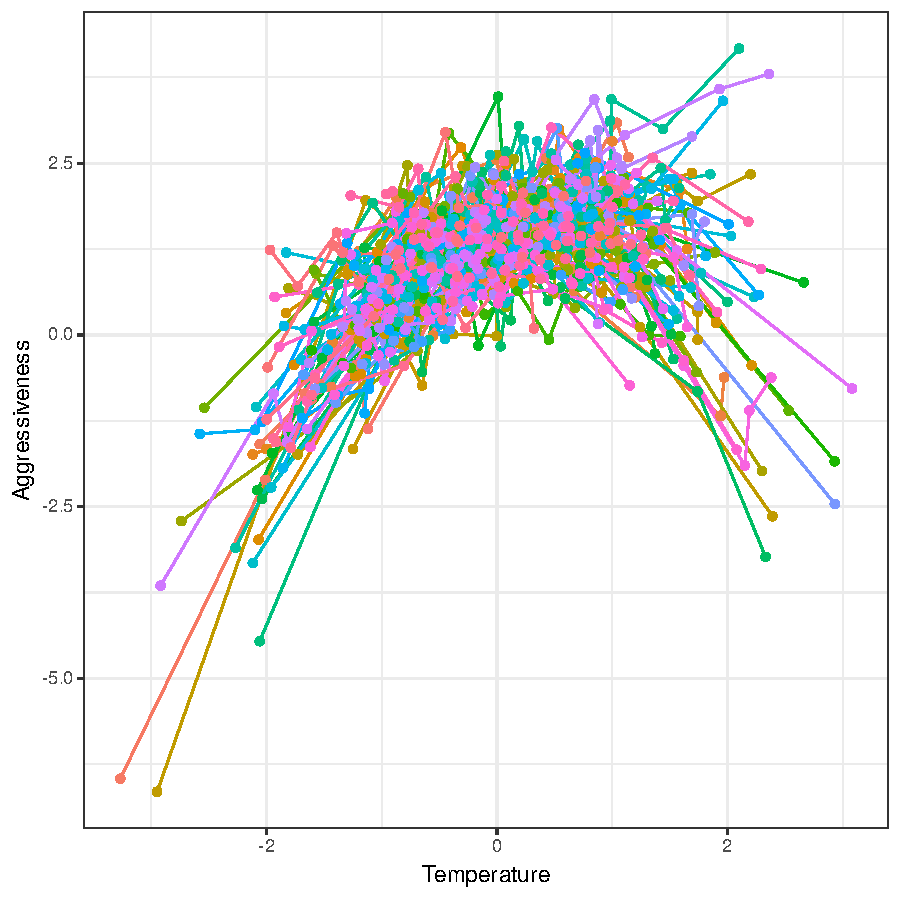
\includegraphics[width = 0.45\textwidth]{Aggressiveness_continuous.pdf}
  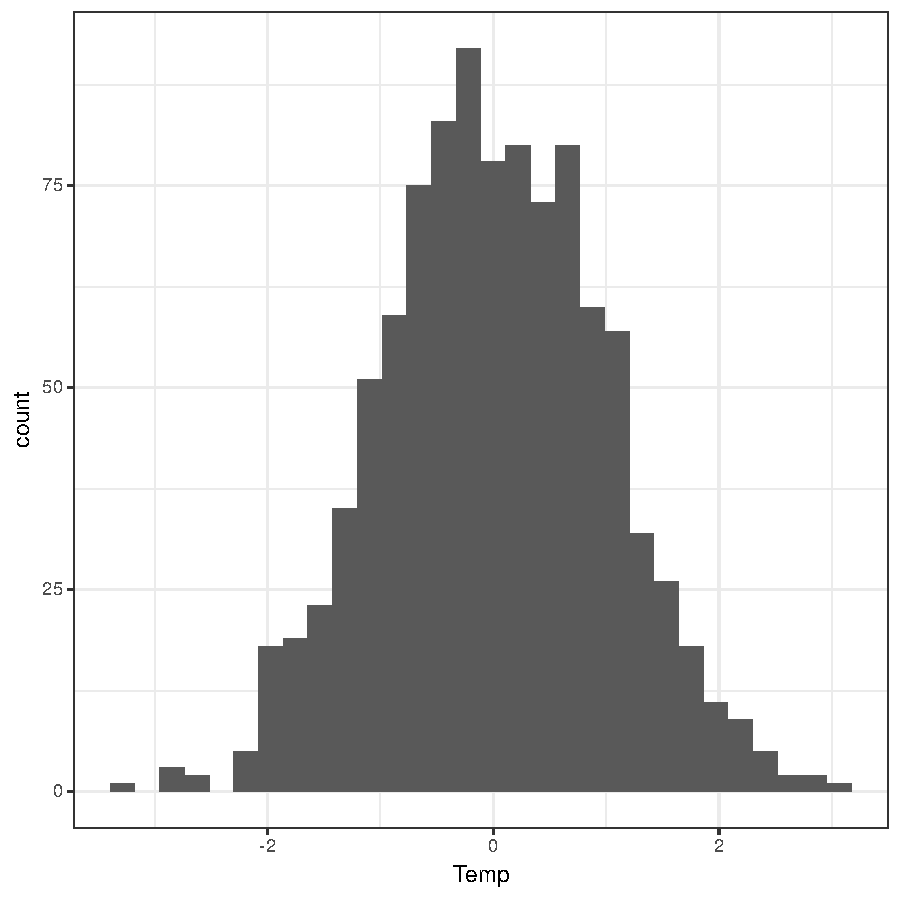
\includegraphics[width = 0.45\textwidth]{Distribution_Temp_continuous.pdf}
  \caption{Left: Dragons aggressiveness according to the temperature at the time of measurement in the field. Right: Distribution of the temperatures at the time of measurements on the dragons in the field.}
  \label{fig_agr_rn_plain_ct}
\end{figure}

\subsubsection{Running the quadratic model}

\paragraph{Preparing the model}
The fist thing that we need to decide is the number of iterations to run the model, and its warm-up phase. We will use the same number of iterations as for the discrete case:
\begin{Rinput}
# Number of independent MCMC chains
n_chains <- 4
# Total number of iterations
n_iter <- 3000
# Number of iterations that will be discarded for the warm-up
n_warm <- 1000
# Thinning interval
n_thin <- 1
\end{Rinput}
Then, we can prepare the formula of the model for \texttt{brms}. Here, we will introduce a new feature: we will provide a matrix of relatedness to our effect, to exactly model the additive genetic variance. This can be easily done in \texttt{brms} by using the \texttt{gr()} function in the formula, and providing the covariance matrix in the \texttt{cov} argument, as follows:
\begin{Rinput}
form_quad <- brmsformula(Aggressiveness ~ Temp + Temp_Sq +
                                          (1 + Temp + Temp_Sq | gr(Individual, cov = A)))
\end{Rinput}
We just provided the formula for a random-slope animal model! Simple, isn't it?

\paragraph{Running the model}
The model is then run, as always, using the \texttt{brm()} function. The only addition here is that we need to provide our relatedness matrix through the \texttt{data2} argument of \texttt{brm()}:
\begin{Rinput}
model_agr <-
        brm(formula   = form_quad,
            data      = tbl_dragon_ct,
            data2     = list(A = A),
            save_pars = save_pars(group = FALSE),
            chains    = n_chains,
            cores     = n_chains,
            seed      = seed,
            iter      = n_iter,
            warmup    = n_warm,
            thin      = n_thin)
summary(model_agr)
plot(model_agr)
\end{Rinput}
\begin{Routput}
 Family: gaussian 
  Links: mu = identity; sigma = identity 
Formula: Aggressiveness ~ Temp + Temp_Sq + (1 + Temp + Temp_Sq | gr(Individual, cov = A)) 
   Data: tbl_dragon_ct (Number of observations: 1000) 
  Draws: 4 chains, each with iter = 3000; warmup = 1000; thin = 1;
         total post-warmup draws = 8000

Multilevel Hyperparameters:
~Individual (Number of levels: 100) 
                       Estimate Est.Error l-95% CI u-95% CI Rhat Bulk_ESS Tail_ESS
sd(Intercept)              0.29      0.04     0.22     0.36 1.00     3316     5332
sd(Temp)                   0.40      0.04     0.33     0.48 1.00     3320     4850
sd(Temp_Sq)                0.27      0.03     0.21     0.33 1.00     2117     3718
cor(Intercept,Temp)       -0.21      0.14    -0.47     0.07 1.00     1466     3343
cor(Intercept,Temp_Sq)    -0.37      0.15    -0.62    -0.06 1.00     1433     2776
cor(Temp,Temp_Sq)          0.24      0.13    -0.03     0.49 1.00     2114     3721

Regression Coefficients:
          Estimate Est.Error l-95% CI u-95% CI Rhat Bulk_ESS Tail_ESS
Intercept     1.49      0.06     1.38     1.60 1.00     4284     5048
Temp          0.48      0.08     0.32     0.63 1.00     2513     3707
Temp_Sq      -0.45      0.05    -0.55    -0.34 1.00     2947     4363

Further Distributional Parameters:
      Estimate Est.Error l-95% CI u-95% CI Rhat Bulk_ESS Tail_ESS
sigma     0.50      0.01     0.48     0.53 1.00     6279     5802

Draws were sampled using sampling(NUTS). For each parameter, Bulk_ESS
and Tail_ESS are effective sample size measures, and Rhat is the potential
scale reduction factor on split chains (at convergence, Rhat = 1).
\end{Routput}
Diagonistics using $\hat{R}$ and the effective sample size seem to signal that everything went smoothly, as does the traces in \autoref{fig_mod_agr_ct}.

\begin{figure}[t!h!]
  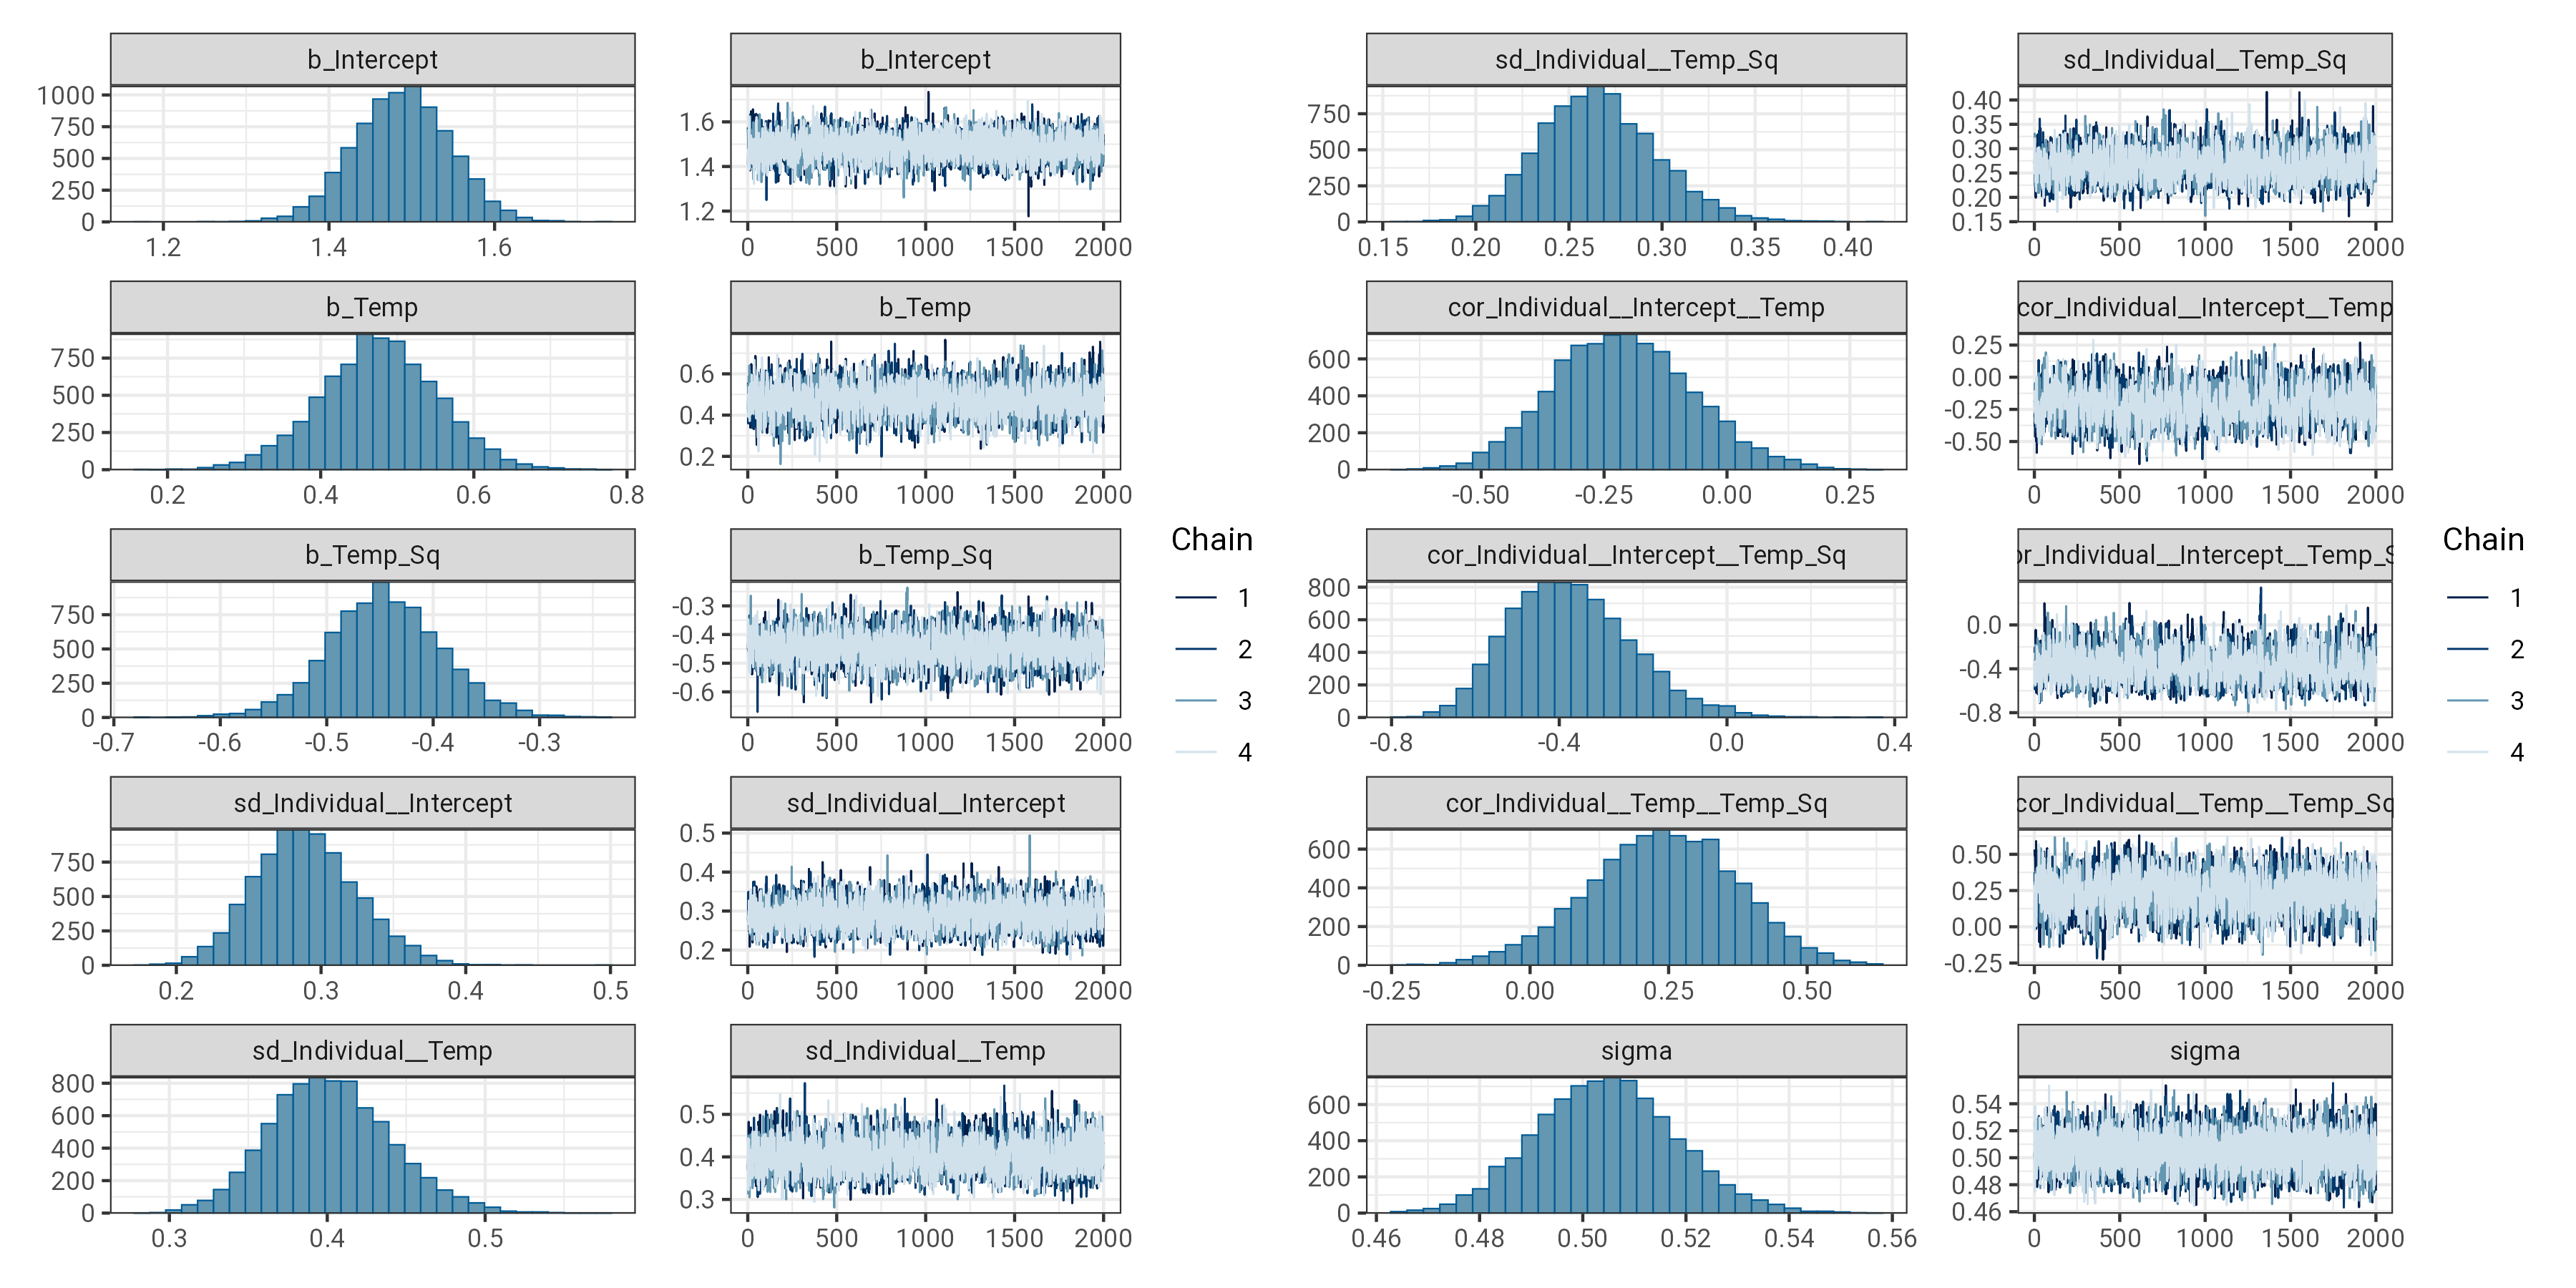
\includegraphics[width = \textwidth]{Aggressiveness_continuous_model.png}
  \caption{Plot of the \texttt{mod\_agr} model. Parameters starting with ``b'' are the fixed effects parameters of the model, and parameters starting with ``sd'' are the standard deviation of the random effects. The parameter ``sigma'' is the residual standard deviation.}
  \label{fig_mod_agr_ct}
\end{figure}

\paragraph{Plotting predictions of the model}
We can superimpose the predictions of the model on the reaction norm data:
\begin{Rinput}
tbl_agr_mod <-
    tbl_dragon_ct |>
    mutate(Predict = predict(model_agr, re_formula = NA) |>
                     as_tibble()) |>
    unpack(Predict) |>
    select(Temp,
           Predict = Estimate,
           Predict_Low = Q2.5,
           Predict_Up  = Q97.5) |>
    summarise(across(starts_with("Predict"), mean),
              .by = Temp)

p_rn_agr <-
    p_aggr +
    geom_ribbon(data = tbl_agr_mod,
                mapping = aes(x = Temp, ymin = Predict_Low, ymax = Predict_Up),
                alpha = 0.3) +
    geom_line(data = tbl_agr_mod,
              mapping = aes(x = Temp, y = Predict),
              linewidth = 1)
\end{Rinput}

\begin{figure}[b!h!]
  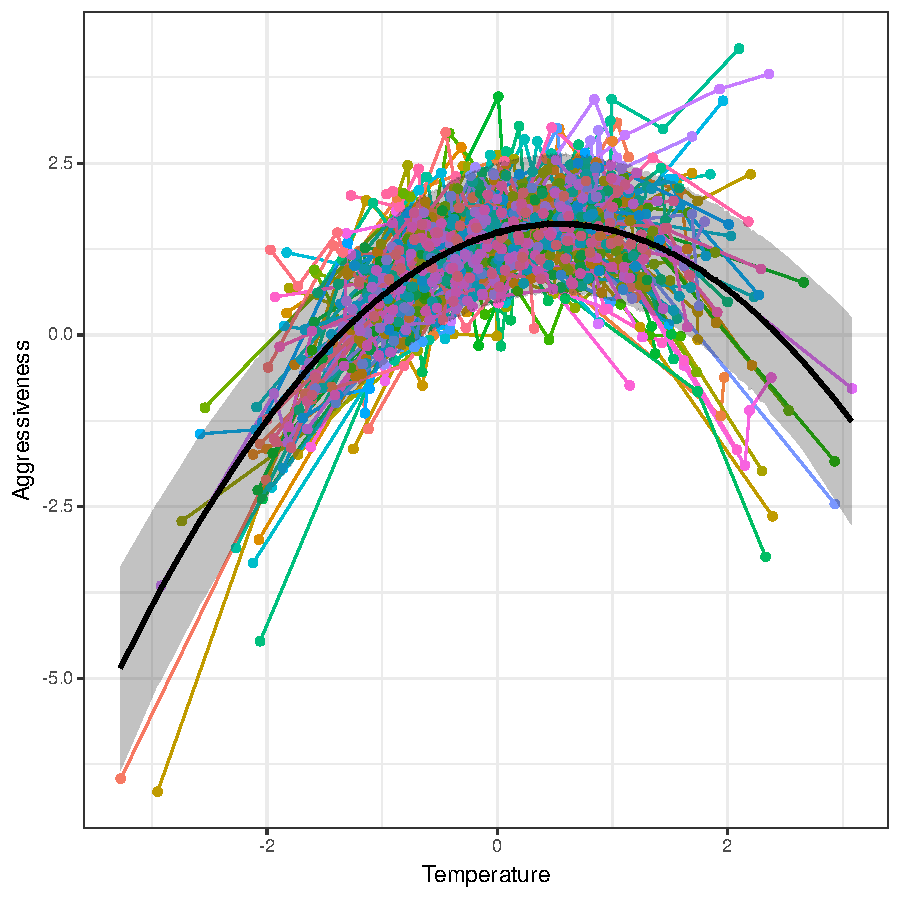
\includegraphics[width = 0.7\textwidth]{Aggressiveness_continuous_pred.pdf}
  \caption{Fit of the quadratic model of the thermal performance from \texttt{mod\_agr}, superimposed over the individual data.}
  \label{fig_pred_agr}
\end{figure}

\subsubsection{Decomposing the variance based on point estimates}

\paragraph{Setting up an environmental vector}
We could directly use data collected on the field for the environment, but this would relatively inefficient, as many values would be close together (and close to the mean), while more extreme values would be a bit lost outside of the range of values.
A more efficient way will be to prepare a sequence of evenly spaced values from -3 to 3 (remember that temperature was mean-centered and scaled to a variance of 1), then we will use the \texttt{dnorm()} function to weight each value according to a normal distribution when calling the \texttt{Reacnorm} functions:
\begin{Rinput}
seq_env <- seq(-3, 3, length.out = 200)
\end{Rinput}
We can also prepare a design matrix based on this sequence of environments:
\begin{Rinput}
seq_X   <- cbind(1, seq_env, seq_env^2)
\end{Rinput}

\paragraph{Extracting the parameters for the model}
We will need the values of the parameters of the quadratic model:
\begin{Rinput}
theta_agr <- fixef(model_agr, robust = TRUE)[ , "Estimate"]
names(theta_agr) <- c("a", "b", "c")
\end{Rinput}
As well as the uncertainty in their estimation:
\begin{Rinput}
S_theta_agr <- vcov(model_agr)
rownames(S_theta_agr) <- colnames(S_theta_agr) <- c("a", "b", "c")
\end{Rinput}
Finally, we need to extract the $\mathbf{G}$-matrix of the parameters and the residual variance:
\begin{Rinput}
G_agr <-
    VarCorr(model_agr, robust = TRUE)[["Individual"]][["cov"]][ , "Estimate", ]
rownames(G_agr) <- colnames(G_agr) <- names(theta_agr)
vr_agr <- VarCorr(model_agr, robust = TRUE)[["residual__"]][["sd"]][ , "Estimate"]^2
\end{Rinput}

\paragraph{Computing $V_{\text{Plas}}$ and the $\pi$-decomposition}
Recalling that when the reaction norm is truly quadratic and/or the environment is normally distributed (here, we have both), then the $\pi$- and $\phi$-decomposition are identical, and thus, we can use \texttt{rn\_phi\_decomp()} here for efficiency (and to be able to correct for the uncertainty in the parameters):
\begin{Rinput}
plas_agr <-
    rn_phi_decomp(theta  = theta_agr,
                  X      = seq_X,
                  S      = S_theta_agr,
                  wt_env = dnorm(seq_env))
plas_agr
\end{Rinput}
\begin{Routput}
     V_Plas        Phi_a     Phi_b     Phi_c      Phi_a_b      Phi_a_c       Phi_b_c
1 0.5566937 4.900216e-32 0.3866837 0.6133163 1.174573e-32 2.951315e-32 -1.090162e-17
\end{Routput}
Note the use of the \texttt{wt\_env} argument using \texttt{dnorm()} to weight each environmental value of the sequence according to a normal distribution.
So, the variance from the slope generates roughly a third of $V_{\text{Plas}}$ ($\pi_{\text{Sl}}=\varphi_{b} = 0.39$), while the curvature generates two-third of it ($\pi_{\text{Cv}}=\varphi_{c} = 0.61$).
Just to be sure, we can compare with the actual $\pi$-decomposition from \texttt{rn\_pi\_decomp()}:
\begin{Rinput}
plas_agr_pi <-
    rn_pi_decomp(theta   = theta_agr,
                    G_theta = G_agr,
                    env     = seq_env,
                    shape   = expression(a + b * x + c * x^2),
                    wt_env  = dnorm(seq_env))
plas_agr_pi
\end{Rinput}
\begin{Routput}
     V_Plas     Pi_Sl     Pi_Cv
1 0.5675039 0.3899418 0.6104246
\end{Routput}
Seems close, but not so close... What is going on? A major difference between the two functions is that \texttt{rn\_pi\_decomp()} cannot use the bias correction due to the uncertainty in the estimation of the parameters (notice that we do not provide \texttt{S\_theta\_agr} to it). What happen if we do not provide to \texttt{rn\_phi\_decomp()}?
\begin{Rinput}
rn_phi_decomp(theta  = theta_agr,
              X      = seq_X,
              wt_env = dnorm(seq_env))
\end{Rinput}
\begin{Routput}
     V_Plas        Phi_a     Phi_b     Phi_c      Phi_a_b     Phi_a_c   Phi_b_c
1 0.5674327 4.814687e-32 0.3895125 0.6104875 1.151877e-32 2.89348e-32 -1.07e-17
\end{Routput}
Now, that is close enough!

\paragraph{Computing the additive genetic variances and their decomposition}
This can be done using, as always, the \texttt{rn\_gen\_decomp()}:
\begin{Rinput}
gen_agr <-
    rn_gen_decomp(theta     = theta_agr,
                  G_theta   = G_agr,
                  X         = seq_X,
                  wt_env    = dnorm(seq_env))
gen_agr
\end{Rinput}
\begin{Routput}
      V_Add        V_A     V_AxE  Gamma_a  Gamma_b  Gamma_c     Gamma_a_b  Gamma_a_c     Gamma_b_c
1 0.3719142 0.09386207 0.2780522 0.223513 0.420248 0.505912 -2.145401e-18 -0.1496729 -1.721787e-18
        Iota_a    Iota_b    Iota_c      Iota_a_b      Iota_a_c      Iota_b_c
1 3.685019e-33 0.5621111 0.4378889 -5.750906e-34 -1.686659e-33 -5.458193e-19
\end{Routput}
Here, we show that, for aggressiveness, the additive genetic variance of plasticity represents a considerable amount of variance ($V_{\text{A}\times\text{E}}=0.28$) compared to the marginal additive genetic variance of the trait ($V_{\text{A}}=0.09$).
The additive genetic variance of plasticity is mostly driven by variation in the slope ($\iota_{b} = 0.56$), while the total additive genetic variance in the reaction norm is mostly driven by the curvature ($\gamma_{c}=0.5$) of the quadratic curve.

\paragraph{Computing the variance-standardised estimates}
As for the discrete case, we can compute the total variance and use it to compute variance-standardised estimates:
\begin{Rinput}
v_tot_agr <- plas_agr[["V_Plas"]] + gen_agr[["V_Add"]] + vr_agr
var_agr <-
    c(P2     = plas_agr[["V_Plas"]] / v_tot_agr,
      h2_RN  = gen_agr[["V_Add"]] / v_tot_agr,
      h2     = gen_agr[["V_A"]] / v_tot_agr,
      h2_I   = gen_agr[["V_AxE"]] / v_tot_agr,
      T2     = (plas_agr[["V_Plas"]] + gen_agr[["V_Add"]]) / v_tot_agr)
\end{Rinput}
\begin{Routput}
        P2      h2_RN         h2       h2_I         T2 
0.47056345 0.31437257 0.07933997 0.23503261 0.78493602 
\end{Routput}

\subsubsection{Decomposing the variance based on posterior distributions}

\paragraph{Why use the posterior distribution?}
The previous section uses computations based on point estimates, but the best way Bayesian way to do it is rather to apply the functions on the posterior distribution of the estimates. This also allows for the computation of the uncertainty in the final estimates.

\paragraph{Getting the posterior distributions of the estimates}
To obtain the posterior distribution of the estimates, we need to set the \texttt{summary} argument to \texttt{FALSE}.
\begin{Rinput}
theta_post_agr <- fixef(model_agr, summary = FALSE)
colnames(theta_post_agr) <- c("a", "b", "c")
vr_post_agr <-
    VarCorr(model_agr, summary = FALSE)[["residual__"]][["sd"]][ , 1]^2
head(theta_post_agr)
\end{Rinput}
\begin{Routput}
    variable
draw        a         b          c
   1 1.574861 0.5398646 -0.4507398
   2 1.507732 0.5543012 -0.4146447
   3 1.453584 0.4524352 -0.4491258
   4 1.458598 0.4481237 -0.4563230
   5 1.471635 0.4477617 -0.4603924
   6 1.521630 0.5193325 -0.4411503
\end{Routput}
For the $\mathbf{G}$-matrix, a bit more work is needed:
\begin{Rinput}
G_post_agr <-
    VarCorr(model_agr, summary = FALSE)[["Individual"]][["cov"]] |>
    # We use apply() to transform the 3-dimensional array into a list
    apply(1, \§§(mat_) { mat_ }, simplify = FALSE) |>
    map(\§§(mat_) { rownames(mat_) <- colnames(mat_) <- c("a", "b", "c"); return(mat_) })
G_post_agr[[1]]
\end{Rinput}
\begin{Routput}
            a           b           c
a  0.07619113 -0.03273076 -0.01878719
b -0.03273076  0.14626823  0.05473105
c -0.01878719  0.05473105  0.07212929
\end{Routput}
Then, we can format everything as a posterior distribution using the \texttt{posterior} package:
\begin{Rinput}
post_agr <- as_draws_df(theta_post_agr)
post_agr[["G"]] <- G_post_agr
post_agr[["V_R"]] <- vr_post_agr
post_agr <- thin_draws(post_agr, thin = nrow(theta_post_agr) / 1000)
# Keep the iteration/chain info to create new posterior objects
post_agr_info <- select(post_agr, starts_with("."))
post_agr
\end{Rinput}
\begin{Routput}
# A draws_df: 250 iterations, 4 chains, and 6 variables
     a    b     c
1  1.6 0.54 -0.45
2  1.5 0.47 -0.47
3  1.6 0.52 -0.38
4  1.5 0.50 -0.43
5  1.5 0.45 -0.46
6  1.5 0.45 -0.39
7  1.6 0.32 -0.51
8  1.5 0.41 -0.46
9  1.5 0.46 -0.47
10 1.5 0.60 -0.36
                                                                                     G  V_R
1                    0.076, -0.033, -0.019, -0.033, 0.146, 0.055, -0.019, 0.055, 0.072 0.25
2                    0.075, -0.023, -0.033, -0.023, 0.140, 0.024, -0.033, 0.024, 0.087 0.27
3                    0.096, -0.061, -0.024, -0.061, 0.220, 0.040, -0.024, 0.040, 0.096 0.26
4  0.08116, -0.01868, -0.03615, -0.01868, 0.20498, 0.00013, -0.03615, 0.00013, 0.07168 0.27
5                    0.059, -0.018, -0.021, -0.018, 0.137, 0.012, -0.021, 0.012, 0.071 0.24
6                    0.094, -0.039, -0.048, -0.039, 0.190, 0.047, -0.048, 0.047, 0.079 0.24
7                    0.051, -0.022, -0.017, -0.022, 0.167, 0.018, -0.017, 0.018, 0.052 0.26
8           0.0567, -0.0041, -0.0102, -0.0041, 0.1683, 0.0238, -0.0102, 0.0238, 0.0613 0.27
9                    0.076, -0.016, -0.018, -0.016, 0.158, 0.038, -0.018, 0.038, 0.072 0.26
10                   0.078, -0.026, -0.034, -0.026, 0.125, 0.029, -0.034, 0.029, 0.060 0.25
               theta
1  1.57, 0.54, -0.45
2  1.47, 0.47, -0.47
3  1.61, 0.52, -0.38
4  1.52, 0.50, -0.43
5  1.46, 0.45, -0.46
6  1.45, 0.45, -0.39
7  1.57, 0.32, -0.51
8  1.53, 0.41, -0.46
9  1.50, 0.46, -0.47
10 1.45, 0.60, -0.36
# ... with 990 more draws
# ... hidden reserved variables {'.chain', '.iteration', '.draw'}
\end{Routput}

\paragraph{Computing $V_{\text{Plas}}$ and its $\pi$-decomposition}
To apply \texttt{rn\_phi\_decomp()} to the posterior distribution of the parameters, we will use the \texttt{map()} function to apply it to the \texttt{theta} column of \texttt{post\_agr} (then some formatting is involved):
\begin{Rinput}
post_plas_agr <-
    map(post_agr[["theta"]],
        \§§(th_) { rn_phi_decomp(theta  = th_,
                      X      = seq_X,
                      S      = S_theta_agr,
                      wt_env = dnorm(seq_env)) },
        .progress = TRUE) |>
    bind_rows()  |>
    select(where(\§§(col_) { abs(mean(col_)) > 10^-5 })) |>
    # Transform into a "draws" object using posterior package
    cbind(post_agr_info) |>
    as_draws_df()
summarise_draws(post_plas_agr)
mcmc_trace(post_plas_agr)
mcmc_areas(post_plas_agr,
           regex_pars = "^V",
           prob = 0.95,
           area_method = "scaled height") /
    mcmc_areas(post_plas_agr,
               regex_pars = "^[^V]",
               prob = 0.95,
               area_method = "scaled height") +
    plot_layout(heights = c(1, 2))
\end{Rinput}
\begin{Routput}
# A tibble: 3 × 10
  variable  mean median     sd   mad    q5   q95  rhat ess_bulk ess_tail
  <chr>    <dbl>  <dbl>  <dbl> <dbl> <dbl> <dbl> <dbl>    <dbl>    <dbl>
1 V_Plas   0.564  0.558 0.0998 0.101 0.411 0.736  1.00    1105.     963.
2 Phi_b    0.391  0.391 0.103  0.103 0.229 0.564  1.00     816.     932.
3 Phi_c    0.609  0.609 0.103  0.103 0.436 0.771  1.00     816.     932.
\end{Routput}
We obtain numbers that are roughly comparable to when we used the point estimates, but this time, we have information about the posterior distribution of those parameters (see \autoref{fig_agr_var_decomp_ct}).

\begin{figure}[t!b!]
  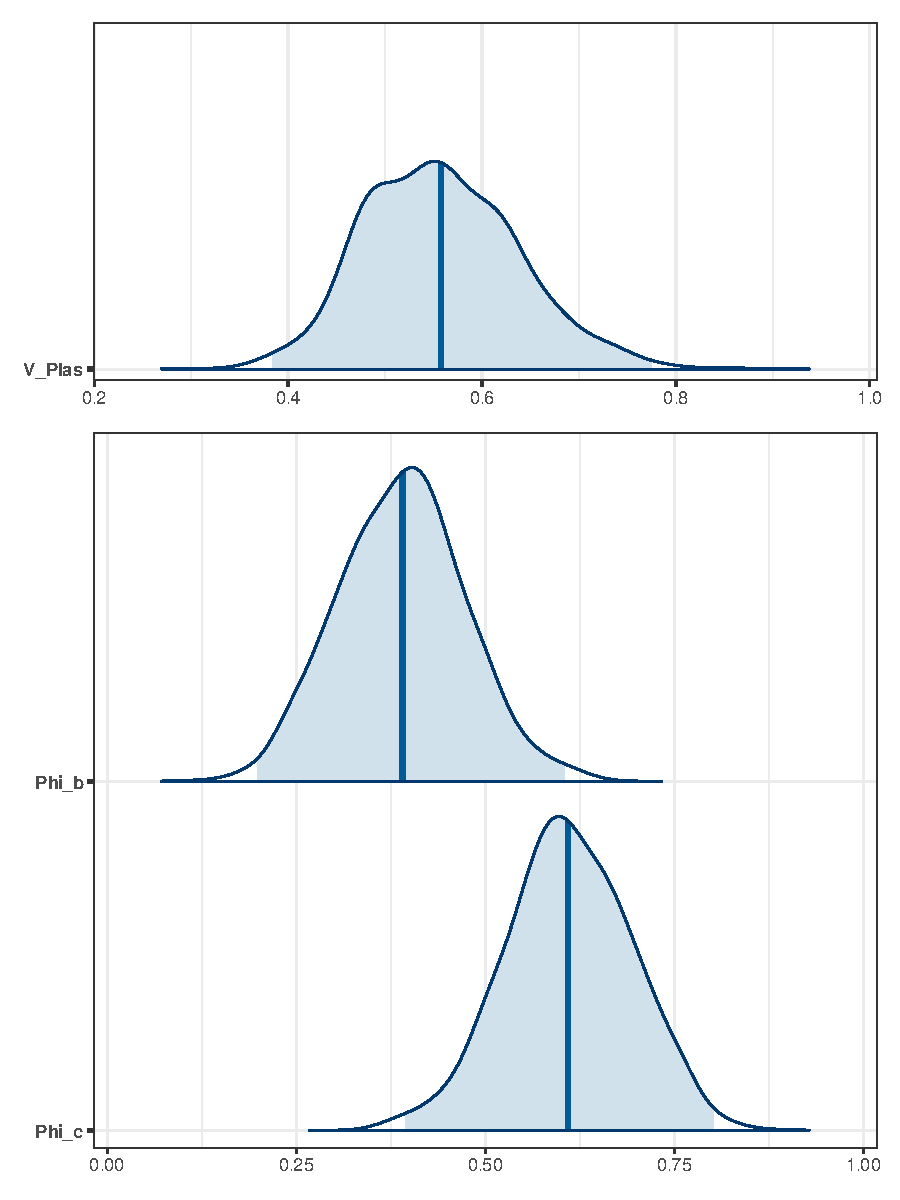
\includegraphics[width = 0.49\textwidth]{Aggressiveness_plas_ct.pdf}
  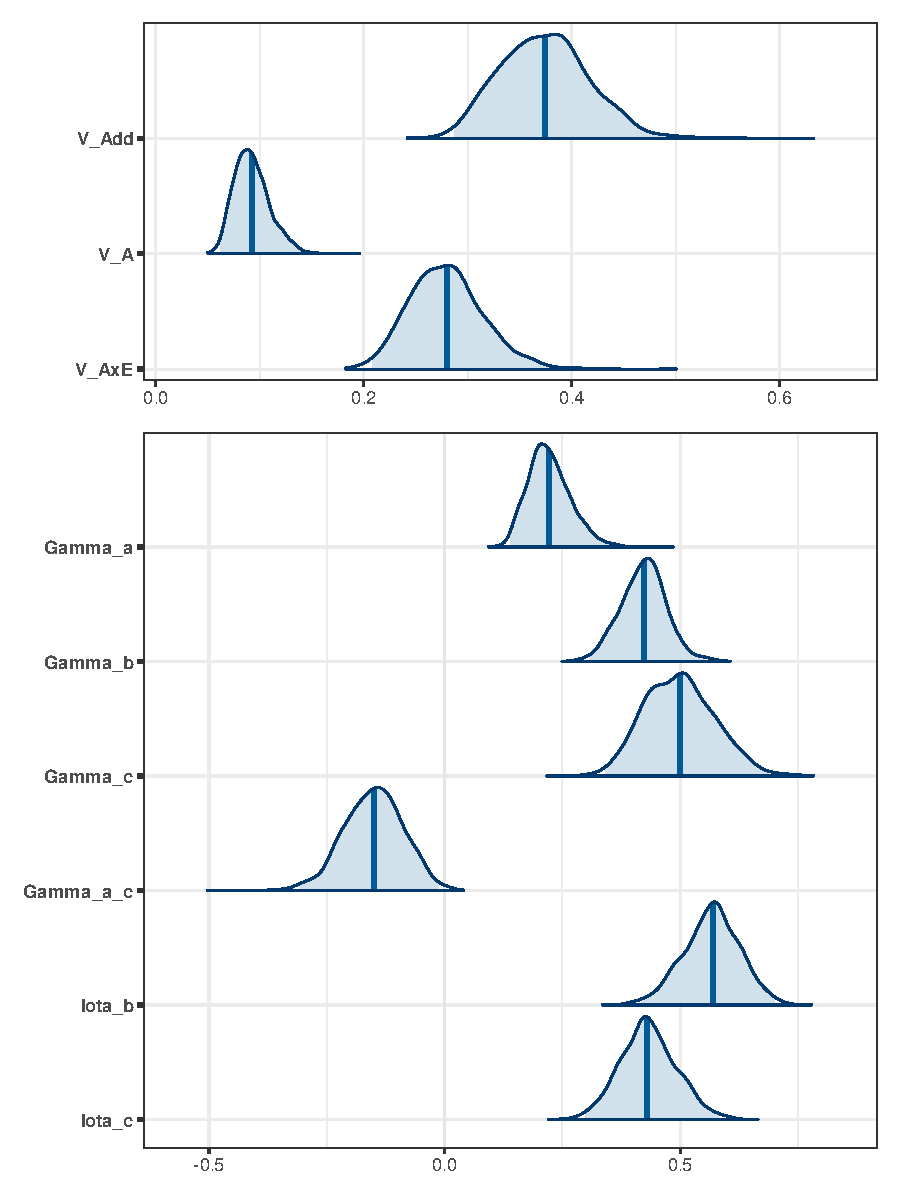
\includegraphics[width = 0.49\textwidth]{Aggressiveness_gen_ct.pdf}
  \caption{Posterior distribution of the variance decomposition of the reaction norm of aggressiveness, based on a quadratic model.}
  \label{fig_agr_var_decomp_ct}
\end{figure}

\paragraph{Computing the additive genetic variances and their decomposition}
Then, we can do the same for \texttt{rn\_gen\_decomp()}, only this time, we need to provide the posterior distibution of the $\mathbf{G}$-matrix as well, so we need to use \texttt{map2()} function, which allows for using 2 arguments:
\begin{Rinput}
post_gen_agr <-
    map2(post_agr[["theta"]], post_agr[["G"]],
     \§§(th_, G_) { rn_gen_decomp(theta = th_,
                                G_theta = G_,
                                X = seq_X,
                                wt_env = dnorm(seq_env)) },
     .progress = TRUE) |>
    bind_rows() |>
    select(where(\§§(col_) { abs(mean(col_)) > 10^-5 })) |>
    cbind(post_agr_info) |>
    as_draws_df()

summarise_draws(post_gen_agr)
mcmc_trace(post_gen_agr)
mcmc_areas(post_gen_agr,
           regex_pars = "^V",
           prob = 0.95,
           area_method = "scaled height") /
    mcmc_areas(post_gen_agr,
               regex_pars = "^[^V]",
               prob = 0.95,
               area_method = "scaled height") +
    plot_layout(heights = c(3, 6))
\end{Rinput}
\begin{Routput}
# A tibble: 9 × 10
  variable     mean  median     sd    mad      q5     q95  rhat ess_bulk ess_tail
  <chr>       <dbl>   <dbl>  <dbl>  <dbl>   <dbl>   <dbl> <dbl>    <dbl>    <dbl>
1 V_Add      0.378   0.375  0.0527 0.0519  0.300   0.464  1.00     1036.     902.
2 V_A        0.0949  0.0926 0.0212 0.0203  0.0658  0.133  1.01      923.     849.
3 V_AxE      0.283   0.280  0.0440 0.0423  0.218   0.360  0.999    1031.     803.
4 Gamma_a    0.227   0.221  0.0545 0.0526  0.150   0.328  1.00      841.     969.
5 Gamma_b    0.423   0.424  0.0601 0.0582  0.324   0.525  1.01      998.     894.
6 Gamma_c    0.503   0.500  0.0897 0.0938  0.365   0.654  1.00     1045.     836.
7 Gamma_a_c -0.153  -0.150  0.0760 0.0755 -0.286  -0.0363 1.00      880.     883.
8 Iota_b     0.565   0.569  0.0726 0.0727  0.440   0.680  1.01     1062.    1016.
9 Iota_c     0.435   0.431  0.0726 0.0727  0.320   0.560  1.01     1062.    1016.
\end{Routput}
Again, the number are close to what we obtained with the posterior estimates, but with the uncertainty around them (see \autoref{fig_agr_var_decomp_ct}).

\paragraph{Computing the total variance and the variance-standardised estimates}
We can obtain the total variance using the \texttt{posterior} package:
\begin{Rinput}
post_var_agr <-
    bind_draws(post_agr, post_plas_agr, post_gen_agr) |>
    subset_draws(variable = c("V_Plas", "V_Add", "V_A", "V_AxE", "V_R")) |>
    mutate_variables(V_Tot = V_Plas + V_Add + V_R)
\end{Rinput}
Now, we have access to the posterior distribution of the total variance in the \texttt{V\_Tot} column. Now, we can use it to compute the variance-standardised estimates:
\begin{Rinput}
post_std_agr <-
    post_var_agr |>
    transmute(P2    = V_Plas / V_Tot,
              H2_RN = V_Add / V_Tot,
              H2    = V_A / V_Tot,
              H2_I  = V_AxE / V_Tot,
              T2    = (V_Plas + V_Add) / V_Tot) |>
    cbind(post_agr_info) |>
    as_draws_df()

summarise_draws(post_std_agr)
mcmc_trace(post_std_agr)
mcmc_areas(post_std_agr,
           prob = 0.95,
           area_method = "scaled height")
\end{Rinput}
\begin{Routput}
# A tibble: 5 × 10
  variable   mean median     sd    mad     q5   q95  rhat ess_bulk ess_tail
  <chr>     <dbl>  <dbl>  <dbl>  <dbl>  <dbl> <dbl> <dbl>    <dbl>    <dbl>
1 P2       0.468  0.470  0.0483 0.0475 0.386  0.545  1.00    1117.    1031.
2 H2_RN    0.317  0.314  0.0401 0.0390 0.257  0.387  1.00    1112.     955.
3 H2       0.0795 0.0779 0.0171 0.0161 0.0549 0.111  1.00     947.     847.
4 H2_I     0.237  0.235  0.0341 0.0341 0.184  0.296  1.00    1070.     880.
5 T2       0.785  0.785  0.0228 0.0222 0.747  0.820  1.00    1011.     913.
\end{Routput}
See \autoref{fig_agr_var_decomp_ct} for the posterior distribution.

\begin{figure}[h!t!]
  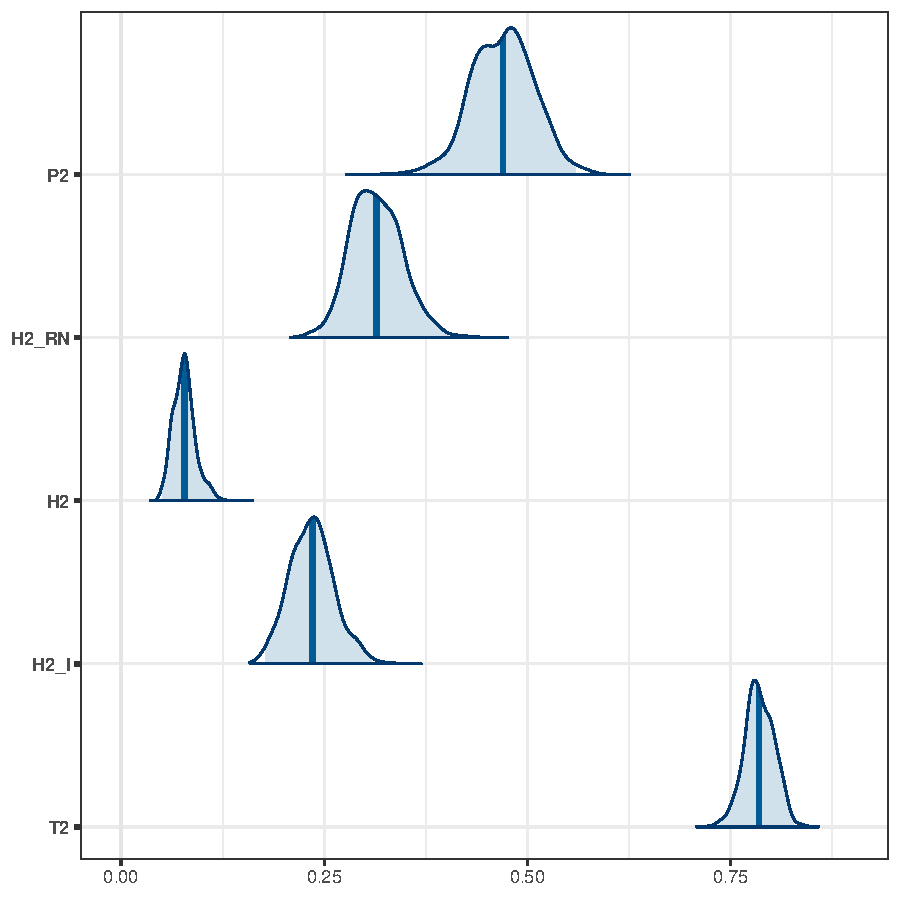
\includegraphics[width = 0.49\textwidth]{Aggressiveness_varstd_ct.pdf}
  \caption{Posterior distribution of the variance-standardised estimates of our variance decomposition of the reaction norm of aggressiveness, based on a quadratic model.}
  \label{fig_agr_var_decomp_ct}
\end{figure}


\subsection{A non-linear reaction norm}

\subsubsection{Data on thermal performance}
There is a column in the dataset that we did not discussed:
\begin{Rinput}
head(dragon_continuous)
\end{Rinput}
\begin{Routput}
  Individual Family   Temp Aggressiveness Performance
1    Ind_001  Fam_1  0.982          2.190       1.080
2    Ind_001  Fam_1  0.469          2.060       1.290
3    Ind_001  Fam_1 -0.108          1.660       0.868
4    Ind_001  Fam_1 -0.213          1.290       0.786
5    Ind_001  Fam_1  1.160          0.698       1.280
6    Ind_001  Fam_1  1.290          1.180       0.980
\end{Routput}
We also have data on locomotive thermal performance, that was measured in the field using a ``transportable'' field corridor with a dummy princess at the end to motivate dragons to run.
If we have a look at the data, we see we recover the same kind of shape than for the experimental case above (see \autoref{fig_tpc_rn_plain_ct}):
\begin{Rinput}
p_tpc <-
    ggplot(tbl_dragon_ct) +
    geom_line(aes(x = Temp, y = Performance, group = Individual, colour = Individual)) +
    geom_point(aes(x = Temp, y = Performance, group = Individual, colour = Individual)) +
    theme(legend.position = "none") +
    xlab("Temperature") + ylab("Performance")
\end{Rinput}
%
\begin{figure}[b!h!t!]
  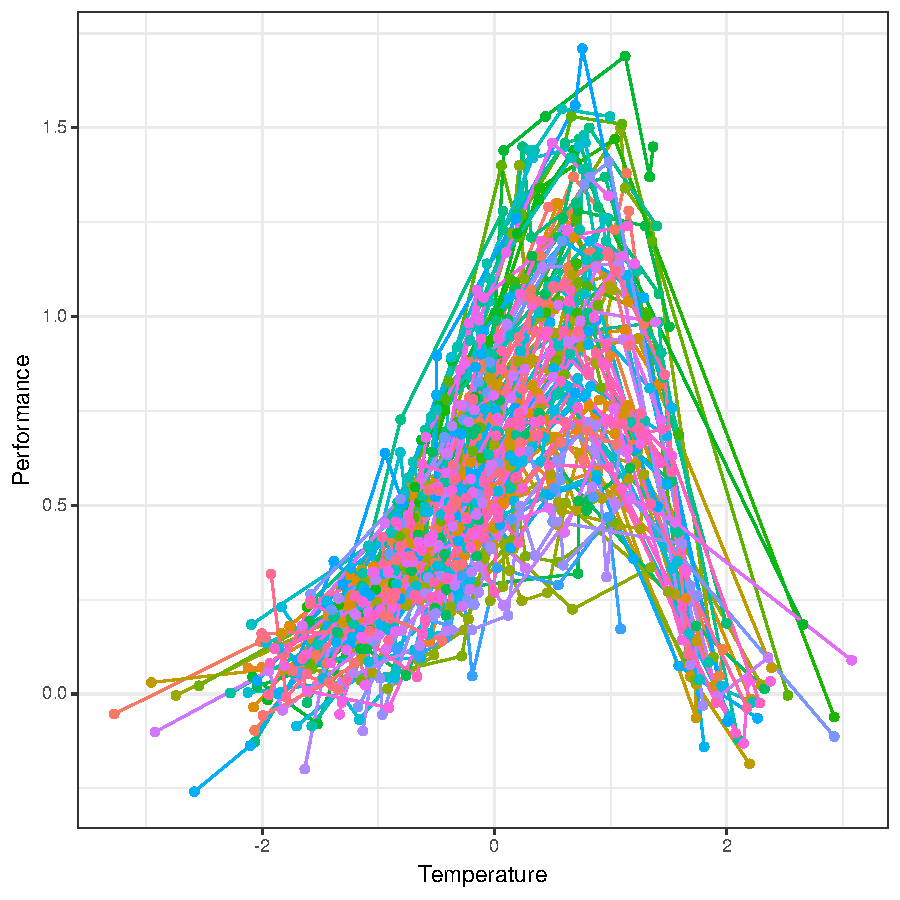
\includegraphics[width = 0.5\textwidth]{TPC_continuous.pdf}
  \caption{Dragons thermal performance, measured as locomotive performance,  according to the temperature at the location of measure in the field}
  \label{fig_tpc_rn_plain_ct}
\end{figure}
So, we will again use \autoref{eq_gg} to model its shape.

\subsubsection{Running the non-linear model}

\paragraph{Preparing the model}
We need to set up the non-linear formula for the model, as we did for the experimental setup in \autoref{subsubsec_nl_mod_ds}, only this time we provide the relatedness matrix \texttt{A} with the \texttt{gr()} function:
\begin{Rinput}
form_nl <- brmsformula(Performance ~ cmax * exp(
                                        - exp(rho * (Temp - xopt) - 6) -       # Gompertz part
                                            sigmagaus * (Temp - xopt)^2        # Gaussian part
                                    ),
                       cmax + xopt ~ 1 + (1 | ID1 | gr(Individual, cov = A)),
                       rho + sigmagaus ~ 1,
                       nl = TRUE)
\end{Rinput}
We will also re-use the same priors and initial values as in \autoref{subsubsec_nl_mod_ds}:
\begin{Rinput}
prior_nl <-
    prior(uniform(0, 100), nlpar = "cmax", lb = 0, ub = 100) +
    prior(uniform(0, 100), nlpar = "rho", lb = 0, ub = 100) +
    prior(uniform(0, 10), nlpar = "sigmagaus", lb = 0, ub = 10)
inits <- rep(list(list(b_cmax      = array(data = 1),
                       b_xopt      = array(data = 0.9),
                       b_rho       = array(data = 8),
                       b_sigmagaus = array(data = 0.4))), 4)
\end{Rinput}
Given that non-linear models are bit more auto-correlated, we will run the model for a little longer:
\begin{Rinput}
# Total number of iterations
n_iter_nl <- 7000
# Number of iterations that will be discarded for the warm-up
n_warm_nl <- 1000
# Thinning interval
n_thin_nl <- 1
\end{Rinput}

\paragraph{Running the model}
Now, we can run the model:
\begin{Rinput}
model_nl_tpc <-
    brm(formula   = form_nl,
        data      = tbl_dragon_ct,
        data2     = list(A = A),
        save_pars = save_pars(group = FALSE),
        chains    = n_chains,
        cores     = n_chains,
        seed      = seed,
        init      = inits,
        prior     = prior_nl,
        iter      = n_iter_nl,
        warmup    = n_warm_nl,
        thin      = n_thin_nl)
summary(model_nl_tpc)
plot(model_nl_tpc)
\end{Rinput}
\begin{Routput}
 Family: gaussian 
  Links: mu = identity; sigma = identity 
Formula: Performance ~ cmax * exp(-exp(rho * (Temp - xopt) - 6) - sigmagaus * (Temp - xopt)^2) 
         cmax ~ 1 + (1 | ID1 | gr(Individual, cov = A))
         xopt ~ 1 + (1 | ID1 | gr(Individual, cov = A))
         rho ~ 1
         sigmagaus ~ 1
   Data: tbl_dragon_ct (Number of observations: 1000) 
  Draws: 4 chains, each with iter = 7000; warmup = 1000; thin = 1;
         total post-warmup draws = 24000

Multilevel Hyperparameters:
~Individual (Number of levels: 100) 
                                   Estimate Est.Error l-95% CI u-95% CI Rhat Bulk_ESS Tail_ESS
sd(cmax_Intercept)                     0.34      0.03     0.30     0.40 1.00     2353     4802
sd(xopt_Intercept)                     0.03      0.01     0.01     0.05 1.00     4643     3856
cor(cmax_Intercept,xopt_Intercept)    -0.23      0.29    -0.76     0.40 1.00    14649     8867

Regression Coefficients:
                    Estimate Est.Error l-95% CI u-95% CI Rhat Bulk_ESS Tail_ESS
cmax_Intercept          0.97      0.06     0.84     1.09 1.00     1226     2574
xopt_Intercept          0.90      0.02     0.86     0.94 1.00    12702    15894
rho_Intercept           8.17      0.30     7.62     8.78 1.00    13466    15788
sigmagaus_Intercept     0.40      0.01     0.37     0.42 1.00    14572    17473

Further Distributional Parameters:
      Estimate Est.Error l-95% CI u-95% CI Rhat Bulk_ESS Tail_ESS
sigma     0.10      0.00     0.09     0.10 1.00    21911    16569

Draws were sampled using sampling(NUTS). For each parameter, Bulk_ESS
and Tail_ESS are effective sample size measures, and Rhat is the potential
scale reduction factor on split chains (at convergence, Rhat = 1).
\end{Routput}
%
\begin{figure}[t!h!]
  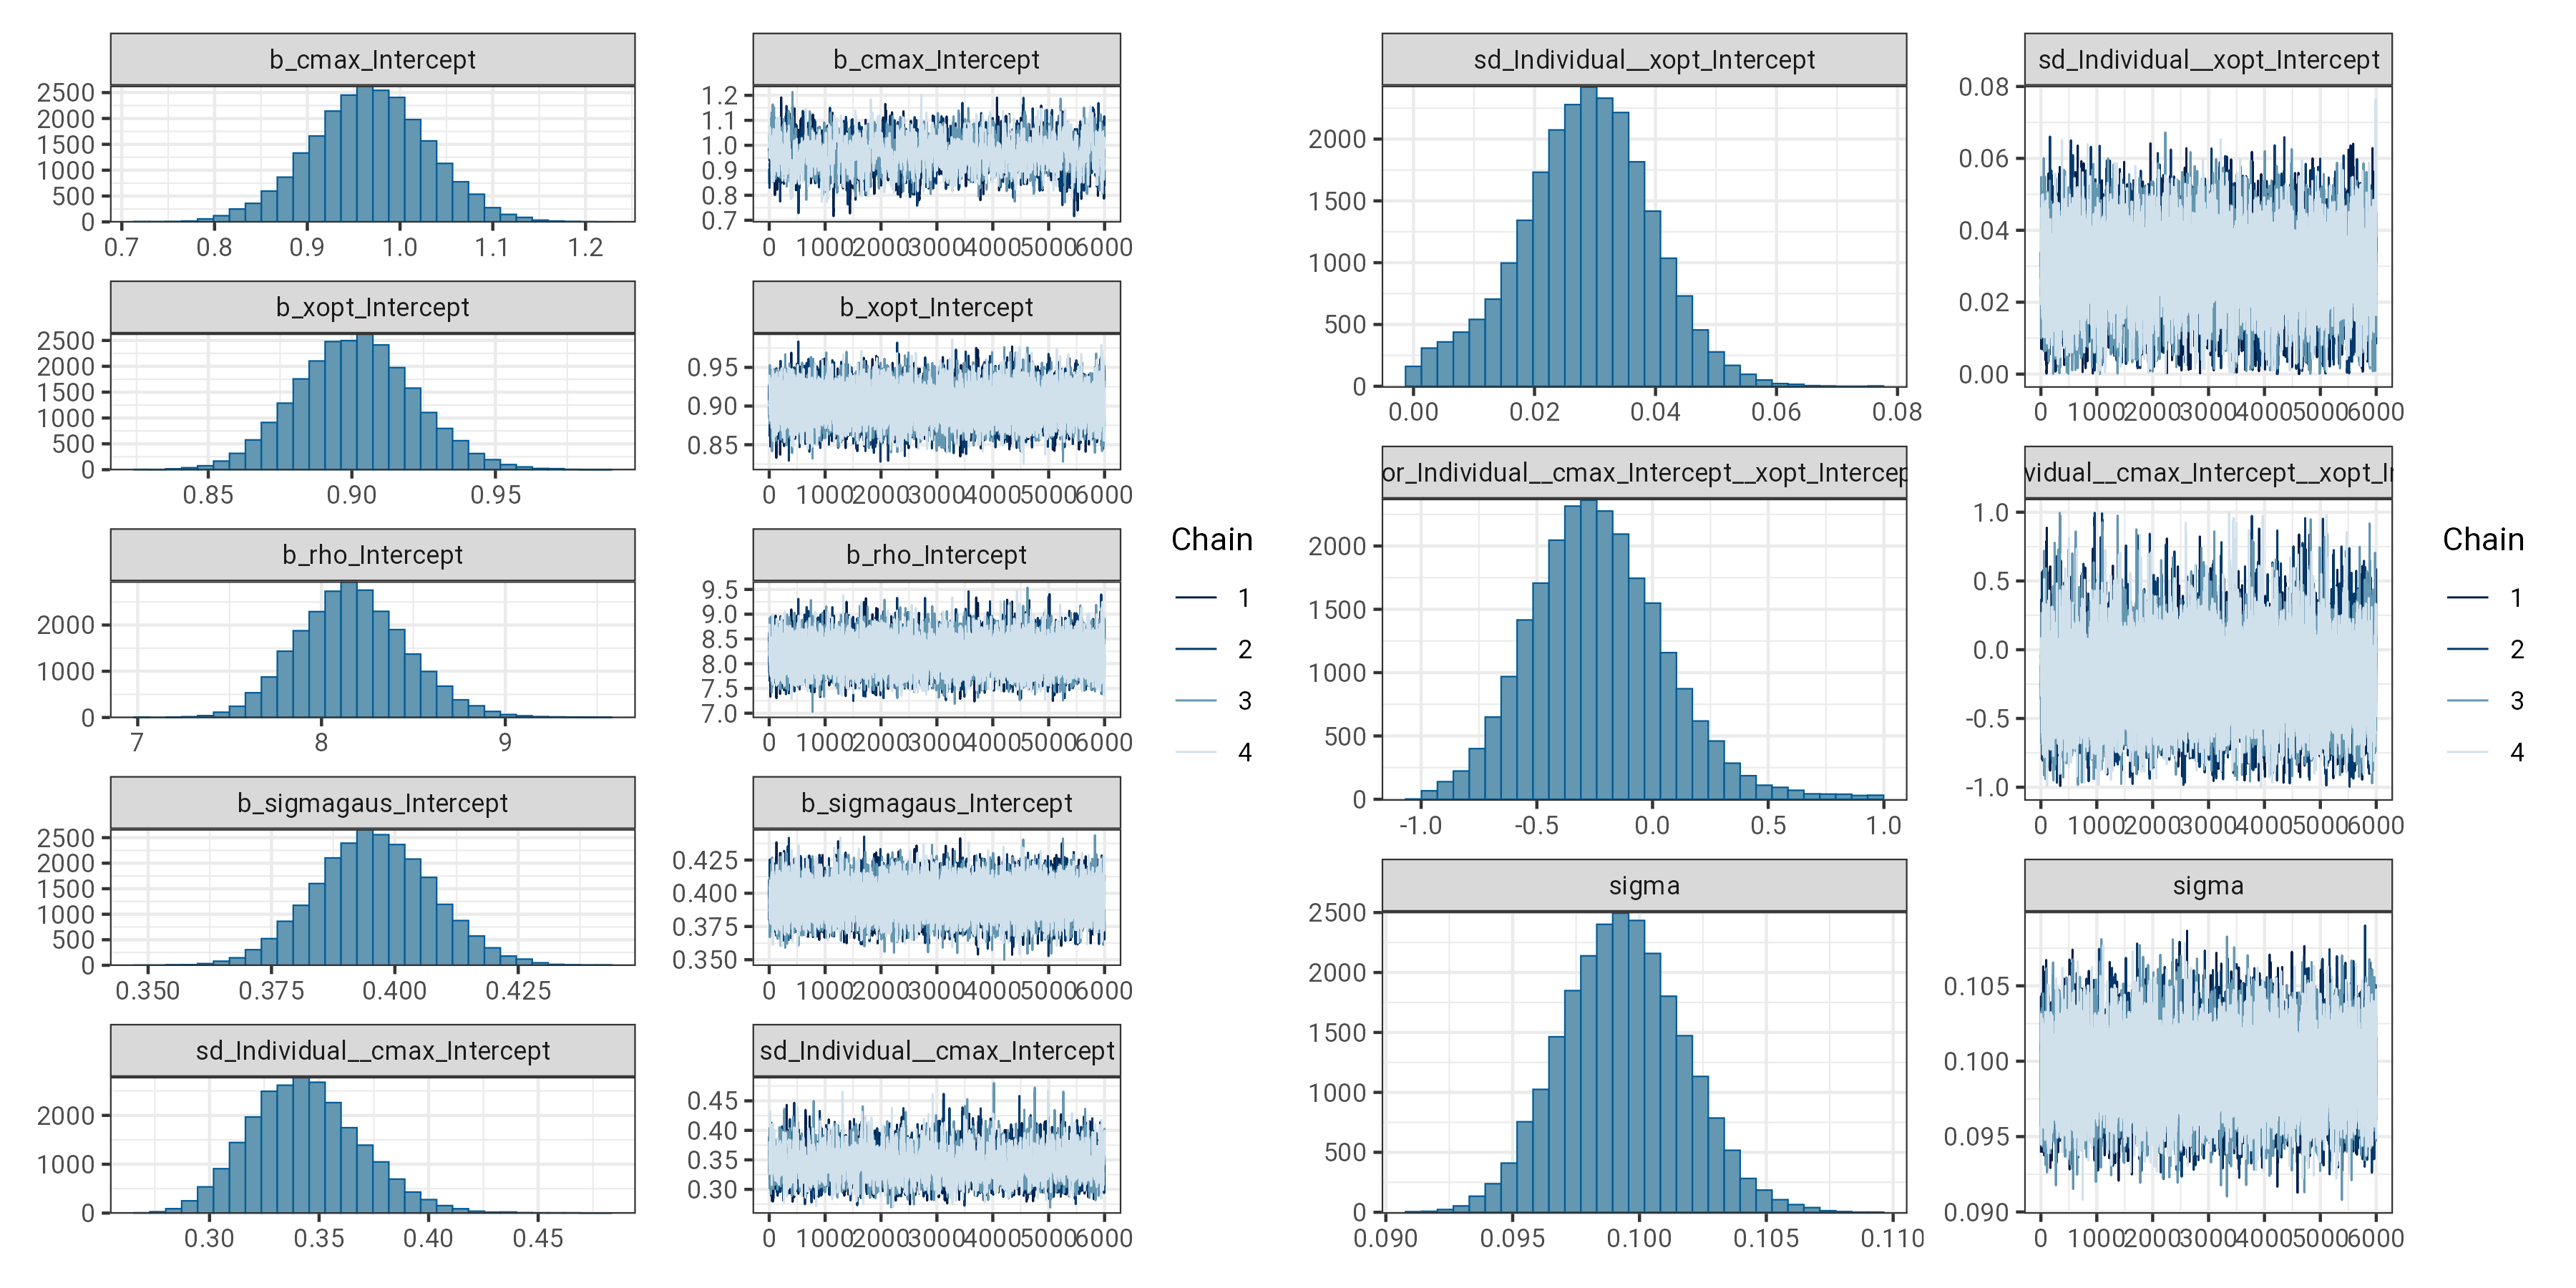
\includegraphics[width = \textwidth]{TPC_nl_model_ct.png}
  \caption{Plot of the \texttt{mod\_nl\_tpc} model. Parameters starting with ``b'' are the fixed effects of the non-linear parameters of the model, and parameters starting with ``sd'' are the standard deviation of the random effects of the non-linear parameters. The parameter ``sigma'' is the residual standard deviation.}
  \label{fig_mod_tpc_nl_ct}
\end{figure}
Diagnostics seem to be OK, as do a graphical check of the traces in \autoref{fig_mod_tpc_nl_ct}. We can also plot the predictions of the model atop the raw data (see \autoref{fig_mod_tpc_nl}):
\begin{Rinput}
tbl_tpc_mod <-
    tbl_dragon_ct |>
    mutate(Predict = predict(model_nl_tpc, re_formula = NA) |>
                     as_tibble()) |>
    unpack(Predict) |>
    select(Temp,
           Predict = Estimate,
           Predict_Low = Q2.5,
           Predict_Up  = Q97.5) |>
    summarise(across(starts_with("Predict"), mean),
              .by = Temp)

p_rn_tpc <-
    p_tpc +
    geom_ribbon(data = tbl_tpc_mod,
                mapping = aes(x = Temp, ymin = Predict_Low, ymax = Predict_Up),
                alpha = 0.3) +
    geom_line(data = tbl_tpc_mod,
              mapping = aes(x = Temp, y = Predict),
              linewidth = 1)
\end{Rinput}
%
\begin{figure}[h!]
  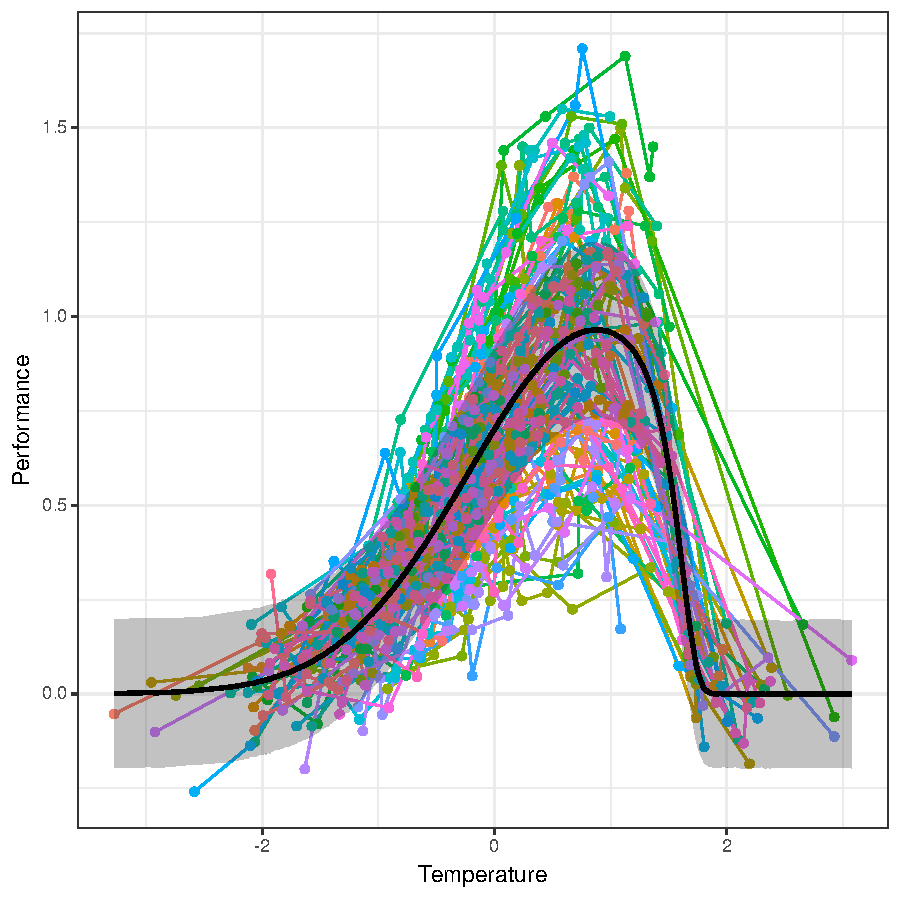
\includegraphics[width = 0.7\textwidth]{TPC_continuous_nonlinear_pred.pdf}
  \caption{Thermal performance individual data, with the non-linear reaction norm predicted by the \texttt{mod\_tpc\_nl} model.}
  \label{fig_pred_tpc_nl_ct}
\end{figure}

\subsubsection{Decomposing the variance based on the posterior distribution}

\paragraph{Getting the parameters}
We can get the posterior distribution of the parameters as for the previous models:
\begin{Rinput}
theta_post_nl_tpc <- fixef(model_nl_tpc, summary = FALSE)
colnames(theta_post_nl_tpc) <- str_remove(colnames(theta_post_nl_tpc), "_Intercept")
G_post_nl_tpc <-
    VarCorr(model_nl_tpc, summary = FALSE)[["Individual"]][["cov"]] |>
    apply(1, \§§(mat_) { mat_ }, simplify = FALSE) |>
    map(\§§(mat_) { 
      rownames(mat_) <- colnames(mat_) <- str_remove(rownames(mat_), "_Intercept"); return(mat_) 
    })
vr_post_nl_tpc <-
    VarCorr(model_nl_tpc, summary = FALSE)[["residual__"]][["sd"]][ , 1]^2
\end{Rinput}
And then, we can subsample the iterations to speed up computation:
\begin{Rinput}
post_nl_tpc <- as_draws_df(theta_post_nl_tpc)
post_nl_tpc[["G"]] <- G_post_nl_tpc
post_nl_tpc[["Theta"]] <-
    post_nl_tpc |>
    select(cmax:sigmagaus) |>
    apply(1, \§§(vec_) { vec_ }, simplify = FALSE)
post_nl_tpc[["V_R"]] <- vr_post_nl_tpc
post_nl_tpc <- thin_draws(post_nl_tpc, thin = nrow(theta_post_nl_tpc) / 1000)
# Keep the iteration/chain info to create new posterior objects
post_nl_tpc_info <- select(post_nl_tpc, starts_with("."))
\end{Rinput}
The last thing we will require is the expression for the shape of reaction norm, using the same parameter names as in our statistical model and a sequence of environments:
\begin{Rinput}
gg_shape <- expression(
    cmax * exp(
        - exp(rho * (x - xopt) - 6) -
            sigmagaus * (x - xopt)^2
    )
)
seq_env <- seq(-3, 3, length.out = 200)
\end{Rinput}

\paragraph{Computing $V_{\text{Plas}}$ and the $\pi$-decomposition}
We can directly compute the $\pi$-decomposition here, because the environment can readily be assumed to be normally distributed. Note that, since the model is non-linear, we cannot compute the $\varphi$-decomposition (or use \texttt{rn\_phi\_decomp()}).
This can take some time, so we will speed things up by parallelising the process using the \texttt{furrr} package, which offers \texttt{future\_*} parallelised version of \texttt{purrr}'s fuction.
We need first to set up this parallelisation. The following code should work in most settings:
\begin{Rinput}
library(furrr)
ncores <- min(parallel::detectCores() - 2, 10)
options(mc.cores = ncores)
plan(multisession)  # plan(multicore) is more efficient for people not on Windows
\end{Rinput}
Now, we just need to call \texttt{future\_map2()} instead of \texttt{map2()}, and R will take care of the parallelisation for us:
\begin{Rinput}
post_pi_nl_tpc <-
    future_map2(post_nl_tpc[["Theta"]], post_nl_tpc[["G"]],
                \§§(th_, G_) { rn_pi_decomp(theta    = th_,
                                          G_theta  = G_,
                                          env      = seq_env,
                                          shape    = gg_shape,
                                          fixed    = c(3, 4),
                                          wt_env   = dnorm(seq_env)) },
                .options=furrr_options(seed = TRUE),
                .progress = TRUE) |>
    bind_rows() |>
    cbind(post_nl_tpc_info) |>
    as_draws_df()
summarise_draws(post_pi_nl_tpc)
mcmc_trace(post_pi_nl_tpc)
mcmc_areas(post_pi_nl_tpc,
           regex_pars = "^V",
           prob = 0.95,
           area_method = "scaled height") /
    mcmc_areas(post_pi_nl_tpc,
               regex_pars = "^[^V]",
               prob = 0.95,
               area_method = "scaled height") +
    plot_layout(heights = c(1, 2))
\end{Rinput}
\begin{Routput}
# A tibble: 3 × 10
  variable   mean median      sd     mad     q5   q95  rhat ess_bulk ess_tail
  <chr>     <dbl>  <dbl>   <dbl>   <dbl>  <dbl> <dbl> <dbl>    <dbl>    <dbl>
1 V_Plas   0.0989 0.0992 0.0138  0.0133  0.0777 0.121 1.00      832.     795.
2 Pi_Sl    0.284  0.285  0.00754 0.00697 0.272  0.297 0.999     973.     638.
3 Pi_Cv    0.310  0.310  0.00726 0.00674 0.299  0.322 1.00      997.     908.
\end{Routput}
Note that we once again used \texttt{wt\_env} to weight environmental values according to a normal distribution, and \texttt{fixed} to state to the fonction that the 3rd (\texttt{rho}) and 4th (\texttt{sigmagaus}) arguments were not allowed to genetically vary.
These results show slightly more variance in the average reaction norm coming from the curvature ($\pi_{\text{Cv}}=0.31$) compared to the contribution of the slope ($\pi_{\text{Sl}}=0.28$).

\begin{figure}[t!b!]
  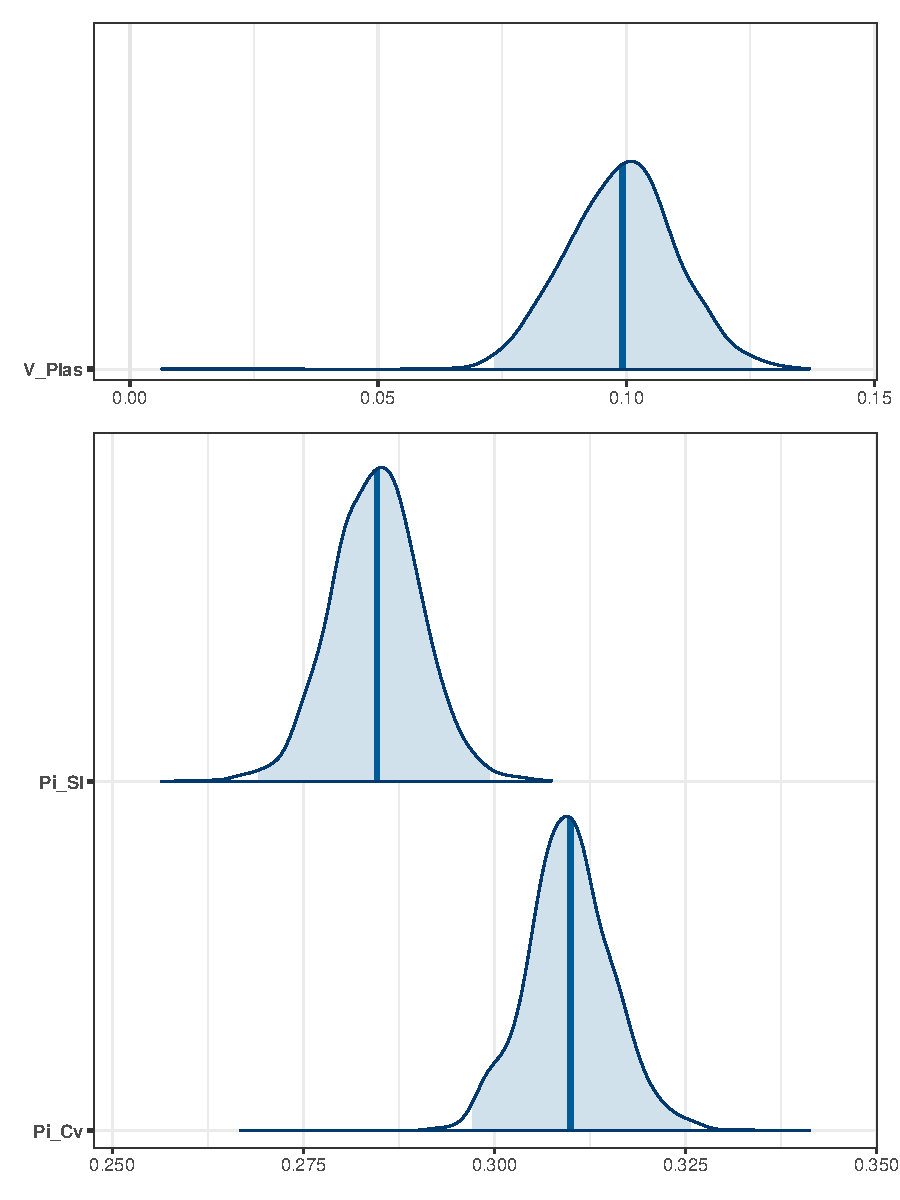
\includegraphics[width = 0.49\textwidth]{TPC_plas_ct.pdf}
  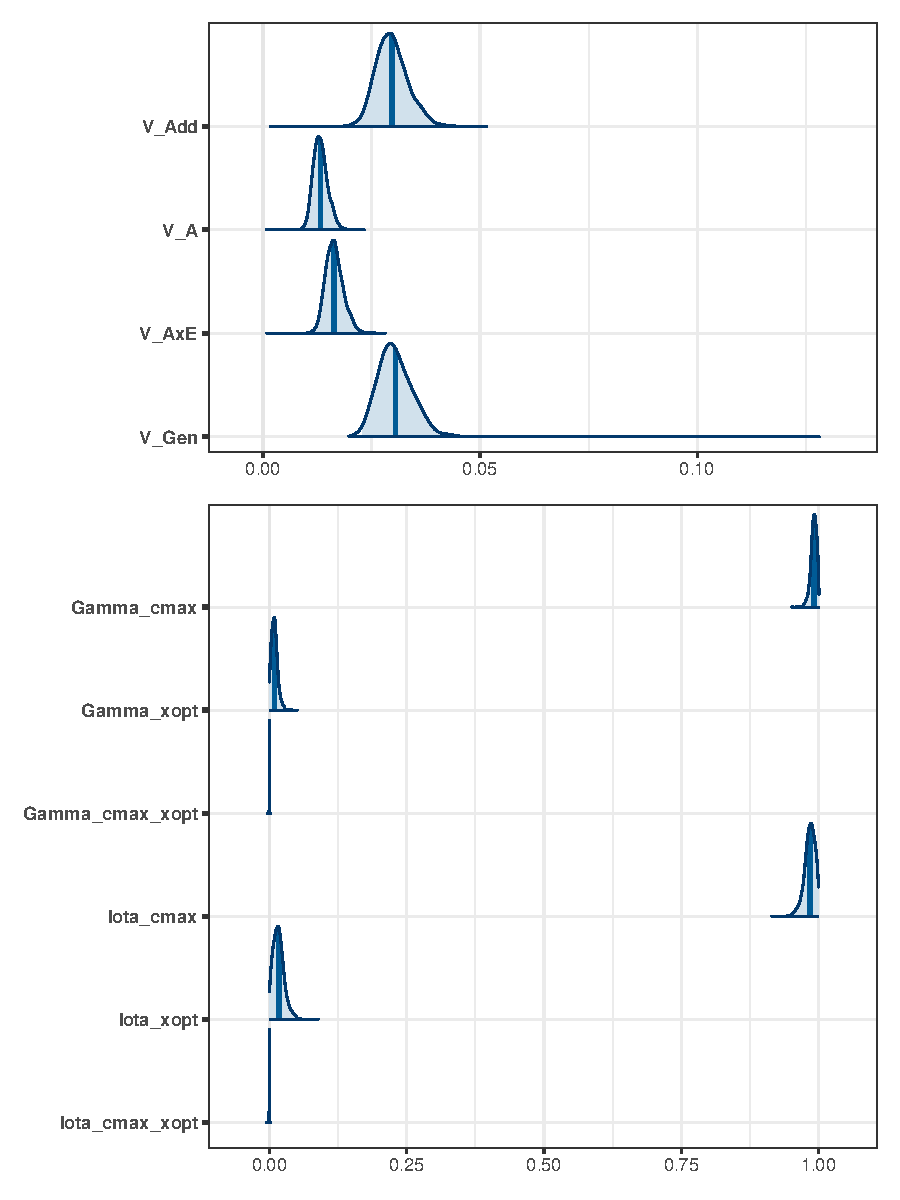
\includegraphics[width = 0.49\textwidth]{TPC_gen_ct.pdf}
  \caption{Posterior distribution of the variance decomposition of the reaction norm of aggressiveness, based on a quadratic model.}
  \label{fig_agr_var_decomp_ct}
\end{figure}

\paragraph{Computing the additive genetic variances and their decomposition}
We will again parallelise the computation of the additive genetic variances using \texttt{furrr}:
\begin{Rinput}
post_gen_nl_tpc <-
    future_map2(post_nl_tpc[["Theta"]], post_nl_tpc[["G"]],
                \§§(th_, G_) { rn_gen_decomp(theta    = th_,
                                           G_theta  = G_,
                                           env      = seq_env,
                                           shape    = gg_shape,
                                           fixed    = c(3, 4)) },
                .options=furrr_options(seed = TRUE),
                .progress = TRUE) |>
    bind_rows() |>
    select(where(\§§(col_) { abs(mean(col_)) > 10^-5 })) |>
    cbind(post_nl_tpc_info) |>
    as_draws_df()
\end{Rinput}
Since the model is non-linear, the total additive genetic variance in the reaction norm ($V_{\text{Add}}$) is not equal to the total (broad-sense) genetic variance in the reaction norm ($V_{\text{Gen}}$). So, to be thorough, we need to add the computation of this $V_{\text{Gen}}$:
\begin{Rinput}
post_gen_nl_tpc[["V_Gen"]] <-
    future_map2_dbl(post_nl_tpc[["Theta"]], post_nl_tpc[["G"]],
                    \§§(th_, G_) { rn_vgen(theta    = th_,
                                        G_theta  = G_,
                                        env      = seq_env,
                                        shape    = gg_shape,
                                        fixed    = c(3, 4),
                                        width    = 8) },
                    .options=furrr_options(seed = TRUE),
                    .progress = TRUE)
\end{Rinput}
Now, we can look at the posterior distribution for all components:
\begin{Rinput}
summarise_draws(post_gen_nl_tpc)
mcmc_trace(post_gen_nl_tpc)
mcmc_areas(post_gen_nl_tpc,
           regex_pars = "^V",
           prob = 0.95,
           area_method = "scaled height") /
    mcmc_areas(post_gen_nl_tpc,
               regex_pars = "^[^V]",
               prob = 0.95,
               area_method = "scaled height") +
    plot_layout(heights = c(3, 6))
\end{Rinput}
\begin{Routput}
# A tibble: 10 × 10
   variable             mean    median       sd      mad        q5       q95  rhat ess_bulk ess_tail
   <chr>               <dbl>     <dbl>    <dbl>    <dbl>     <dbl>     <dbl> <dbl>    <dbl>    <dbl>
 1 V_Add            0.0301    0.0297   0.00476  0.00444   0.0234     3.82e-2 0.999    1087.     955.
 2 V_A              0.0134    0.0133   0.00216  0.00199   0.0104     1.71e-2 0.999    1094.     955.
 3 V_AxE            0.0166    0.0164   0.00261  0.00244   0.0130     2.10e-2 0.999    1081.     994.
 4 Gamma_cmax       0.990     0.991    0.00701  0.00655   0.977      9.99e-1 0.999    1102.     944.
 5 Gamma_xopt       0.0102    0.00922  0.00715  0.00661   0.000682   2.34e-2 0.999    1100.     944.
 6 Gamma_cmax_xopt -0.000307 -0.000161 0.000428 0.000216 -0.00121   -1.04e-6 1.00     1031.    1038.
 7 Iota_cmax        0.982     0.984    0.0125   0.0117    0.959      9.99e-1 0.999    1100.     932.
 8 Iota_xopt        0.0184    0.0167   0.0127   0.0118    0.00125    4.16e-2 0.999    1100.     941.
 9 Iota_cmax_xopt  -0.000514 -0.000263 0.000724 0.000358 -0.00208   -2.08e-7 1.00     1042.    1036.
10 V_Gen            0.0317    0.0305   0.00798  0.00488   0.0240     4.13e-2 1.00     1002.     941.
\end{Routput}
Clearly, whether we look at the contribution of the parameter $C$ to the total additive genetic variance ($\gamma_{C}=0.99$) or to the additive genetic variance of plasticity ($\iota_{C}=0.98$), its importance is extremely strong in this case.

\paragraph{Computing the total variance and the variance-standardised estimates}
We can compute the total variance and the variance-standardised estimates as in the quadratic case:
\begin{Rinput}
post_var_nl_tpc <-
    bind_draws(post_nl_tpc, post_pi_nl_tpc, post_gen_nl_tpc) |>
    subset_draws(variable = c("V_Plas", "V_Gen", "V_Add", "V_A", "V_AxE", "V_R")) |>
    mutate_variables(V_Tot = V_Plas + V_Gen + V_R)

post_std_nl_tpc <-
    post_var_nl_tpc |>
    transmute(P2            = V_Plas / V_Tot,
              Broad_H2_RN   = V_Gen / V_Tot,
              H2_RN         = V_Add / V_Tot,
              H2            = V_A / V_Tot,
              H2_I          = V_AxE / V_Tot,
              T2            = (V_Plas + V_Gen) / V_Tot) |>
    cbind(post_nl_tpc_info) |>
    as_draws_df()
summarise_draws(post_std_nl_tpc)
mcmc_trace(post_std_nl_tpc)
mcmc_areas(post_std_nl_tpc,
           prob = 0.95,
           area_method = "scaled height")
\end{Rinput}
\begin{Routput}
# A tibble: 6 × 10
  variable      mean median      sd     mad     q5   q95  rhat ess_bulk ess_tail
  <chr>        <dbl>  <dbl>   <dbl>   <dbl>  <dbl> <dbl> <dbl>    <dbl>    <dbl>
1 P2          0.703  0.710  0.0532  0.0375  0.632  0.762 0.999     970.     884.
2 Broad_H2_RN 0.226  0.218  0.0506  0.0358  0.172  0.292 0.999    1000.     884.
3 H2_RN       0.215  0.212  0.0356  0.0328  0.166  0.276 1.00     1074.     954.
4 H2          0.0961 0.0945 0.0162  0.0149  0.0738 0.124 1.00     1071.     954.
5 H2_I        0.119  0.117  0.0195  0.0177  0.0919 0.152 1.00     1076.     954.
6 T2          0.929  0.930  0.00860 0.00799 0.915  0.942 1.00      850.     806.
\end{Routput}
In this case, most of the variance comes from the average shape of reaction norm ($P^{2}_{\text{RN}}=0.7$), and the reaction norm explains most of the variation in the phenotypic trait ($T^{2}_{\text{RN}}=0.93$). The difference between the broad- and narrow-sense heritabilities ($H^{2}_{\text{RN}}=0.23$ v. $h^{2}_{\text{RN}}=0.22$) is not strong. The heritability in the reaction norm is roughly split into the marginal heritability of the trait ($h^{2}=0.10$) and the heritability of plasticity ($h^{2}_{\text{I}}=0.12$).
%
\begin{figure}[h!t!]
  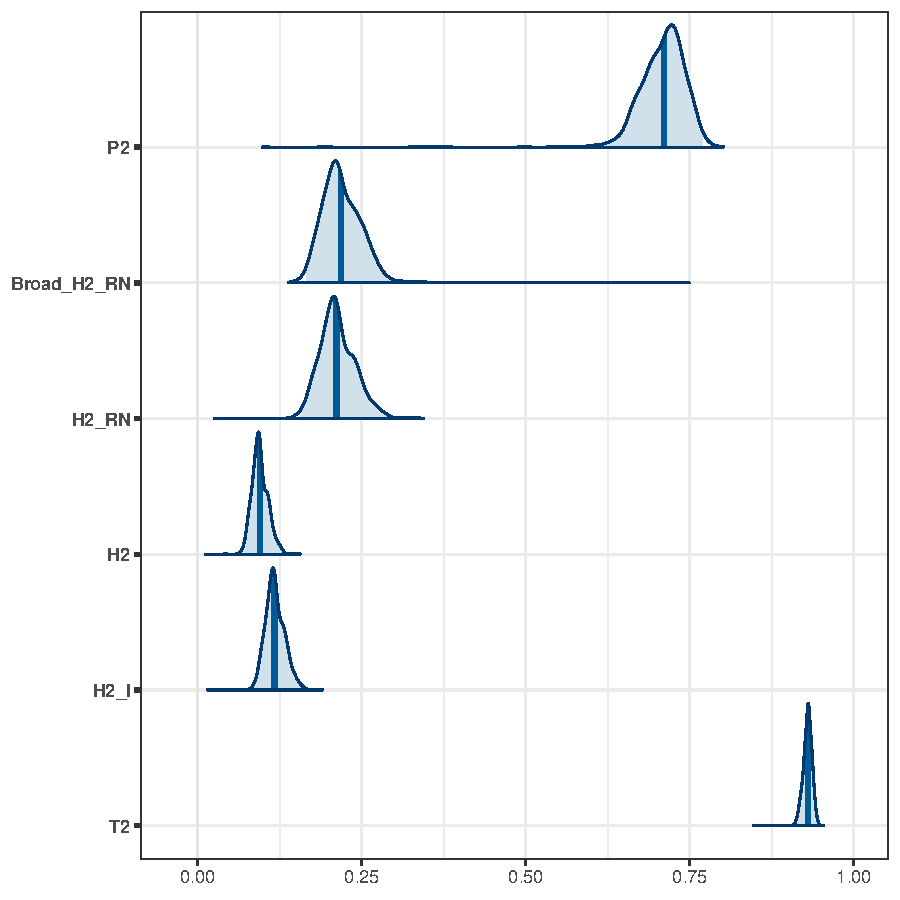
\includegraphics[width = 0.49\textwidth]{TPC_varstd_ct.pdf}
  \caption{Posterior distribution of the variance-standardised estimates of our variance decomposition of the reaction norm of TPC, based on a non-linear model.}
  \label{fig_agr_var_decomp_ct}
\end{figure}

\begin{multicols}{2}
  \begin{singlespace}
    \small
    \printbibliography
  \end{singlespace}
\end{multicols}
\end{document}
